
\documentclass{article}

\usepackage{microtype}
\usepackage{graphicx}
\usepackage{subcaption}

\usepackage{booktabs} %

\usepackage{hyperref}


\newcommand{\theHalgorithm}{\arabic{algorithm}}


\usepackage[accepted]{icml2024}

\usepackage{amsmath}
\usepackage{amssymb}
\usepackage{mathtools}
\usepackage{amsthm}

\usepackage[capitalize,noabbrev]{cleveref}


\theoremstyle{plain}
\newtheorem{theorem}{Theorem}[section]
\newtheorem{proposition}[theorem]{Proposition}
\newtheorem{lemma}[theorem]{Lemma}
\newtheorem{corollary}[theorem]{Corollary}
\theoremstyle{definition}
\newtheorem{definition}[theorem]{Definition}
\newtheorem{assumption}[theorem]{Assumption}
\theoremstyle{remark}
\newtheorem{remark}[theorem]{Remark}
%%%%% NEW MATH DEFINITIONS %%%%%

\usepackage{amsmath,amsfonts,bm}

% Mark sections of captions for referring to divisions of figures
\newcommand{\figleft}{{\em (Left)}}
\newcommand{\figcenter}{{\em (Center)}}
\newcommand{\figright}{{\em (Right)}}
\newcommand{\figtop}{{\em (Top)}}
\newcommand{\figbottom}{{\em (Bottom)}}
\newcommand{\captiona}{{\em (a)}}
\newcommand{\captionb}{{\em (b)}}
\newcommand{\captionc}{{\em (c)}}
\newcommand{\captiond}{{\em (d)}}

% Highlight a newly defined term
\newcommand{\newterm}[1]{{\bf #1}}


% Figure reference, lower-case.
\def\figref#1{figure~\ref{#1}}
% Figure reference, capital. For start of sentence
\def\Figref#1{Figure~\ref{#1}}
\def\twofigref#1#2{figures \ref{#1} and \ref{#2}}
\def\quadfigref#1#2#3#4{figures \ref{#1}, \ref{#2}, \ref{#3} and \ref{#4}}
% Section reference, lower-case.
\def\secref#1{section~\ref{#1}}
% Section reference, capital.
\def\Secref#1{Section~\ref{#1}}
% Reference to two sections.
\def\twosecrefs#1#2{sections \ref{#1} and \ref{#2}}
% Reference to three sections.
\def\secrefs#1#2#3{sections \ref{#1}, \ref{#2} and \ref{#3}}
% Reference to an equation, lower-case.
% \def\eqref#1{equation~\ref{#1}}
\def\eqref#1{(\ref{#1})}
% Reference to an equation, upper case
\def\Eqref#1{Equation~\ref{#1}}
% A raw reference to an equation---avoid using if possible
\def\plaineqref#1{\ref{#1}}
% Reference to a chapter, lower-case.
\def\chapref#1{chapter~\ref{#1}}
% Reference to an equation, upper case.
\def\Chapref#1{Chapter~\ref{#1}}
% Reference to a range of chapters
\def\rangechapref#1#2{chapters\ref{#1}--\ref{#2}}
% Reference to an algorithm, lower-case.
\def\algref#1{algorithm~\ref{#1}}
% Reference to an algorithm, upper case.
\def\Algref#1{Algorithm~\ref{#1}}
\def\twoalgref#1#2{algorithms \ref{#1} and \ref{#2}}
\def\Twoalgref#1#2{Algorithms \ref{#1} and \ref{#2}}
% Reference to a part, lower case
\def\partref#1{part~\ref{#1}}
% Reference to a part, upper case
\def\Partref#1{Part~\ref{#1}}
\def\twopartref#1#2{parts \ref{#1} and \ref{#2}}

\def\ceil#1{\lceil #1 \rceil}
\def\floor#1{\lfloor #1 \rfloor}
\def\1{\bm{1}}
\newcommand{\train}{\mathcal{D}}
\newcommand{\valid}{\mathcal{D_{\mathrm{valid}}}}
\newcommand{\test}{\mathcal{D_{\mathrm{test}}}}

\def\eps{{\epsilon}}


% Random variables
\def\reta{{\textnormal{$\eta$}}}
\def\ra{{\textnormal{a}}}
\def\rb{{\textnormal{b}}}
\def\rc{{\textnormal{c}}}
\def\rd{{\textnormal{d}}}
\def\re{{\textnormal{e}}}
\def\rf{{\textnormal{f}}}
\def\rg{{\textnormal{g}}}
\def\rh{{\textnormal{h}}}
\def\ri{{\textnormal{i}}}
\def\rj{{\textnormal{j}}}
\def\rk{{\textnormal{k}}}
\def\rl{{\textnormal{l}}}
% rm is already a command, just don't name any random variables m
\def\rn{{\textnormal{n}}}
\def\ro{{\textnormal{o}}}
\def\rp{{\textnormal{p}}}
\def\rq{{\textnormal{q}}}
\def\rr{{\textnormal{r}}}
\def\rs{{\textnormal{s}}}
\def\rt{{\textnormal{t}}}
\def\ru{{\textnormal{u}}}
\def\rv{{\textnormal{v}}}
\def\rw{{\textnormal{w}}}
\def\rx{{\textnormal{x}}}
\def\ry{{\textnormal{y}}}
\def\rz{{\textnormal{z}}}

% Random vectors
\def\rvepsilon{{\mathbf{\epsilon}}}
\def\rvtheta{{\mathbf{\theta}}}
\def\rva{{\mathbf{a}}}
\def\rvb{{\mathbf{b}}}
\def\rvc{{\mathbf{c}}}
\def\rvd{{\mathbf{d}}}
\def\rve{{\mathbf{e}}}
\def\rvf{{\mathbf{f}}}
\def\rvg{{\mathbf{g}}}
\def\rvh{{\mathbf{h}}}
\def\rvu{{\mathbf{i}}}
\def\rvj{{\mathbf{j}}}
\def\rvk{{\mathbf{k}}}
\def\rvl{{\mathbf{l}}}
\def\rvm{{\mathbf{m}}}
\def\rvn{{\mathbf{n}}}
\def\rvo{{\mathbf{o}}}
\def\rvp{{\mathbf{p}}}
\def\rvq{{\mathbf{q}}}
\def\rvr{{\mathbf{r}}}
\def\rvs{{\mathbf{s}}}
\def\rvt{{\mathbf{t}}}
\def\rvu{{\mathbf{u}}}
\def\rvv{{\mathbf{v}}}
\def\rvw{{\mathbf{w}}}
\def\rvx{{\mathbf{x}}}
\def\rvy{{\mathbf{y}}}
\def\rvz{{\mathbf{z}}}

% Elements of random vectors
\def\erva{{\textnormal{a}}}
\def\ervb{{\textnormal{b}}}
\def\ervc{{\textnormal{c}}}
\def\ervd{{\textnormal{d}}}
\def\erve{{\textnormal{e}}}
\def\ervf{{\textnormal{f}}}
\def\ervg{{\textnormal{g}}}
\def\ervh{{\textnormal{h}}}
\def\ervi{{\textnormal{i}}}
\def\ervj{{\textnormal{j}}}
\def\ervk{{\textnormal{k}}}
\def\ervl{{\textnormal{l}}}
\def\ervm{{\textnormal{m}}}
\def\ervn{{\textnormal{n}}}
\def\ervo{{\textnormal{o}}}
\def\ervp{{\textnormal{p}}}
\def\ervq{{\textnormal{q}}}
\def\ervr{{\textnormal{r}}}
\def\ervs{{\textnormal{s}}}
\def\ervt{{\textnormal{t}}}
\def\ervu{{\textnormal{u}}}
\def\ervv{{\textnormal{v}}}
\def\ervw{{\textnormal{w}}}
\def\ervx{{\textnormal{x}}}
\def\ervy{{\textnormal{y}}}
\def\ervz{{\textnormal{z}}}

% Random matrices
\def\rmA{{\mathbf{A}}}
\def\rmB{{\mathbf{B}}}
\def\rmC{{\mathbf{C}}}
\def\rmD{{\mathbf{D}}}
\def\rmE{{\mathbf{E}}}
\def\rmF{{\mathbf{F}}}
\def\rmG{{\mathbf{G}}}
\def\rmH{{\mathbf{H}}}
\def\rmI{{\mathbf{I}}}
\def\rmJ{{\mathbf{J}}}
\def\rmK{{\mathbf{K}}}
\def\rmL{{\mathbf{L}}}
\def\rmM{{\mathbf{M}}}
\def\rmN{{\mathbf{N}}}
\def\rmO{{\mathbf{O}}}
\def\rmP{{\mathbf{P}}}
\def\rmQ{{\mathbf{Q}}}
\def\rmR{{\mathbf{R}}}
\def\rmS{{\mathbf{S}}}
\def\rmT{{\mathbf{T}}}
\def\rmU{{\mathbf{U}}}
\def\rmV{{\mathbf{V}}}
\def\rmW{{\mathbf{W}}}
\def\rmX{{\mathbf{X}}}
\def\rmY{{\mathbf{Y}}}
\def\rmZ{{\mathbf{Z}}}

% Elements of random matrices
\def\ermA{{\textnormal{A}}}
\def\ermB{{\textnormal{B}}}
\def\ermC{{\textnormal{C}}}
\def\ermD{{\textnormal{D}}}
\def\ermE{{\textnormal{E}}}
\def\ermF{{\textnormal{F}}}
\def\ermG{{\textnormal{G}}}
\def\ermH{{\textnormal{H}}}
\def\ermI{{\textnormal{I}}}
\def\ermJ{{\textnormal{J}}}
\def\ermK{{\textnormal{K}}}
\def\ermL{{\textnormal{L}}}
\def\ermM{{\textnormal{M}}}
\def\ermN{{\textnormal{N}}}
\def\ermO{{\textnormal{O}}}
\def\ermP{{\textnormal{P}}}
\def\ermQ{{\textnormal{Q}}}
\def\ermR{{\textnormal{R}}}
\def\ermS{{\textnormal{S}}}
\def\ermT{{\textnormal{T}}}
\def\ermU{{\textnormal{U}}}
\def\ermV{{\textnormal{V}}}
\def\ermW{{\textnormal{W}}}
\def\ermX{{\textnormal{X}}}
\def\ermY{{\textnormal{Y}}}
\def\ermZ{{\textnormal{Z}}}

% Vectors
\def\vzero{{\bm{0}}}
\def\vone{{\bm{1}}}
\def\vmu{{\bm{\mu}}}
\def\vtheta{{\bm{\theta}}}
\def\va{{\bm{a}}}
\def\vb{{\bm{b}}}
\def\vc{{\bm{c}}}
\def\vd{{\bm{d}}}
\def\ve{{\bm{e}}}
\def\vf{{\bm{f}}}
\def\vg{{\bm{g}}}
\def\vh{{\bm{h}}}
\def\vi{{\bm{i}}}
\def\vj{{\bm{j}}}
\def\vk{{\bm{k}}}
\def\vl{{\bm{l}}}
\def\vm{{\bm{m}}}
\def\vn{{\bm{n}}}
\def\vo{{\bm{o}}}
\def\vp{{\bm{p}}}
\def\vq{{\bm{q}}}
\def\vr{{\bm{r}}}
\def\vs{{\bm{s}}}
\def\vt{{\bm{t}}}
\def\vu{{\bm{u}}}
\def\vv{{\bm{v}}}
\def\vw{{\bm{w}}}
\def\vx{{\bm{x}}}
\def\vy{{\bm{y}}}
\def\vz{{\bm{z}}}

% Elements of vectors
\def\evalpha{{\alpha}}
\def\evbeta{{\beta}}
\def\evepsilon{{\epsilon}}
\def\evlambda{{\lambda}}
\def\evomega{{\omega}}
\def\evmu{{\mu}}
\def\evpsi{{\psi}}
\def\evsigma{{\sigma}}
\def\evtheta{{\theta}}
\def\eva{{a}}
\def\evb{{b}}
\def\evc{{c}}
\def\evd{{d}}
\def\eve{{e}}
\def\evf{{f}}
\def\evg{{g}}
\def\evh{{h}}
\def\evi{{i}}
\def\evj{{j}}
\def\evk{{k}}
\def\evl{{l}}
\def\evm{{m}}
\def\evn{{n}}
\def\evo{{o}}
\def\evp{{p}}
\def\evq{{q}}
\def\evr{{r}}
\def\evs{{s}}
\def\evt{{t}}
\def\evu{{u}}
\def\evv{{v}}
\def\evw{{w}}
\def\evx{{x}}
\def\evy{{y}}
\def\evz{{z}}

% Matrix
\def\mA{{\bm{A}}}
\def\mB{{\bm{B}}}
\def\mC{{\bm{C}}}
\def\mD{{\bm{D}}}
\def\mE{{\bm{E}}}
\def\mF{{\bm{F}}}
\def\mG{{\bm{G}}}
\def\mH{{\bm{H}}}
\def\mI{{\bm{I}}}
\def\mJ{{\bm{J}}}
\def\mK{{\bm{K}}}
\def\mL{{\bm{L}}}
\def\mM{{\bm{M}}}
\def\mN{{\bm{N}}}
\def\mO{{\bm{O}}}
\def\mP{{\bm{P}}}
\def\mQ{{\bm{Q}}}
\def\mR{{\bm{R}}}
\def\mS{{\bm{S}}}
\def\mT{{\bm{T}}}
\def\mU{{\bm{U}}}
\def\mV{{\bm{V}}}
\def\mW{{\bm{W}}}
\def\mX{{\bm{X}}}
\def\mY{{\bm{Y}}}
\def\mZ{{\bm{Z}}}
\def\mBeta{{\bm{\beta}}}
\def\mPhi{{\bm{\Phi}}}
\def\mLambda{{\bm{\Lambda}}}
\def\mSigma{{\bm{\Sigma}}}

% Tensor
\DeclareMathAlphabet{\mathsfit}{\encodingdefault}{\sfdefault}{m}{sl}
\SetMathAlphabet{\mathsfit}{bold}{\encodingdefault}{\sfdefault}{bx}{n}
\newcommand{\tens}[1]{\bm{\mathsfit{#1}}}
\def\tA{{\tens{A}}}
\def\tB{{\tens{B}}}
\def\tC{{\tens{C}}}
\def\tD{{\tens{D}}}
\def\tE{{\tens{E}}}
\def\tF{{\tens{F}}}
\def\tG{{\tens{G}}}
\def\tH{{\tens{H}}}
\def\tI{{\tens{I}}}
\def\tJ{{\tens{J}}}
\def\tK{{\tens{K}}}
\def\tL{{\tens{L}}}
\def\tM{{\tens{M}}}
\def\tN{{\tens{N}}}
\def\tO{{\tens{O}}}
\def\tP{{\tens{P}}}
\def\tQ{{\tens{Q}}}
\def\tR{{\tens{R}}}
\def\tS{{\tens{S}}}
\def\tT{{\tens{T}}}
\def\tU{{\tens{U}}}
\def\tV{{\tens{V}}}
\def\tW{{\tens{W}}}
\def\tX{{\tens{X}}}
\def\tY{{\tens{Y}}}
\def\tZ{{\tens{Z}}}


% Graph
\def\gA{{\mathcal{A}}}
\def\gB{{\mathcal{B}}}
\def\gC{{\mathcal{C}}}
\def\gD{{\mathcal{D}}}
\def\gE{{\mathcal{E}}}
\def\gF{{\mathcal{F}}}
\def\gG{{\mathcal{G}}}
\def\gH{{\mathcal{H}}}
\def\gI{{\mathcal{I}}}
\def\gJ{{\mathcal{J}}}
\def\gK{{\mathcal{K}}}
\def\gL{{\mathcal{L}}}
\def\gM{{\mathcal{M}}}
\def\gN{{\mathcal{N}}}
\def\gO{{\mathcal{O}}}
\def\gP{{\mathcal{P}}}
\def\gQ{{\mathcal{Q}}}
\def\gR{{\mathcal{R}}}
\def\gS{{\mathcal{S}}}
\def\gT{{\mathcal{T}}}
\def\gU{{\mathcal{U}}}
\def\gV{{\mathcal{V}}}
\def\gW{{\mathcal{W}}}
\def\gX{{\mathcal{X}}}
\def\gY{{\mathcal{Y}}}
\def\gZ{{\mathcal{Z}}}

% Sets
\def\sA{{\mathbb{A}}}
\def\sB{{\mathbb{B}}}
\def\sC{{\mathbb{C}}}
\def\sD{{\mathbb{D}}}
% Don't use a set called E, because this would be the same as our symbol
% for expectation.
\def\sF{{\mathbb{F}}}
\def\sG{{\mathbb{G}}}
\def\sH{{\mathbb{H}}}
\def\sI{{\mathbb{I}}}
\def\sJ{{\mathbb{J}}}
\def\sK{{\mathbb{K}}}
\def\sL{{\mathbb{L}}}
\def\sM{{\mathbb{M}}}
\def\sN{{\mathbb{N}}}
\def\sO{{\mathbb{O}}}
\def\sP{{\mathbb{P}}}
\def\sQ{{\mathbb{Q}}}
\def\sR{{\mathbb{R}}}
\def\sS{{\mathbb{S}}}
\def\sT{{\mathbb{T}}}
\def\sU{{\mathbb{U}}}
\def\sV{{\mathbb{V}}}
\def\sW{{\mathbb{W}}}
\def\sX{{\mathbb{X}}}
\def\sY{{\mathbb{Y}}}
\def\sZ{{\mathbb{Z}}}

% Entries of a matrix
\def\emLambda{{\Lambda}}
\def\emA{{A}}
\def\emB{{B}}
\def\emC{{C}}
\def\emD{{D}}
\def\emE{{E}}
\def\emF{{F}}
\def\emG{{G}}
\def\emH{{H}}
\def\emI{{I}}
\def\emJ{{J}}
\def\emK{{K}}
\def\emL{{L}}
\def\emM{{M}}
\def\emN{{N}}
\def\emO{{O}}
\def\emP{{P}}
\def\emQ{{Q}}
\def\emR{{R}}
\def\emS{{S}}
\def\emT{{T}}
\def\emU{{U}}
\def\emV{{V}}
\def\emW{{W}}
\def\emX{{X}}
\def\emY{{Y}}
\def\emZ{{Z}}
\def\emSigma{{\Sigma}}

% entries of a tensor
% Same font as tensor, without \bm wrapper
\newcommand{\etens}[1]{\mathsfit{#1}}
\def\etLambda{{\etens{\Lambda}}}
\def\etA{{\etens{A}}}
\def\etB{{\etens{B}}}
\def\etC{{\etens{C}}}
\def\etD{{\etens{D}}}
\def\etE{{\etens{E}}}
\def\etF{{\etens{F}}}
\def\etG{{\etens{G}}}
\def\etH{{\etens{H}}}
\def\etI{{\etens{I}}}
\def\etJ{{\etens{J}}}
\def\etK{{\etens{K}}}
\def\etL{{\etens{L}}}
\def\etM{{\etens{M}}}
\def\etN{{\etens{N}}}
\def\etO{{\etens{O}}}
\def\etP{{\etens{P}}}
\def\etQ{{\etens{Q}}}
\def\etR{{\etens{R}}}
\def\etS{{\etens{S}}}
\def\etT{{\etens{T}}}
\def\etU{{\etens{U}}}
\def\etV{{\etens{V}}}
\def\etW{{\etens{W}}}
\def\etX{{\etens{X}}}
\def\etY{{\etens{Y}}}
\def\etZ{{\etens{Z}}}

% The true underlying data generating distribution
\newcommand{\pdata}{p_{\rm{data}}}
% The empirical distribution defined by the training set
\newcommand{\ptrain}{\hat{p}_{\rm{data}}}
\newcommand{\Ptrain}{\hat{P}_{\rm{data}}}
% The model distribution
\newcommand{\pmodel}{p_{\rm{model}}}
\newcommand{\Pmodel}{P_{\rm{model}}}
\newcommand{\ptildemodel}{\tilde{p}_{\rm{model}}}
% Stochastic autoencoder distributions
\newcommand{\pencode}{p_{\rm{encoder}}}
\newcommand{\pdecode}{p_{\rm{decoder}}}
\newcommand{\precons}{p_{\rm{reconstruct}}}

\newcommand{\laplace}{\mathrm{Laplace}} % Laplace distribution

\newcommand{\E}{\mathbb{E}}
\newcommand{\Ls}{\mathcal{L}}
\newcommand{\R}{\mathbb{R}}
\newcommand{\emp}{\tilde{p}}
\newcommand{\lr}{\alpha}
\newcommand{\reg}{\lambda}
\newcommand{\rect}{\mathrm{rectifier}}
\newcommand{\softmax}{\mathrm{softmax}}
\newcommand{\sigmoid}{\sigma}
\newcommand{\softplus}{\zeta}
\newcommand{\KL}{D_{\mathrm{KL}}}
\newcommand{\Var}{\mathrm{Var}}
\newcommand{\standarderror}{\mathrm{SE}}
\newcommand{\Cov}{\mathrm{Cov}}
% Wolfram Mathworld says $L^2$ is for function spaces and $\ell^2$ is for vectors
% But then they seem to use $L^2$ for vectors throughout the site, and so does
% wikipedia.
\newcommand{\normlzero}{L^0}
\newcommand{\normlone}{L^1}
\newcommand{\normltwo}{L^2}
\newcommand{\normlp}{L^p}
\newcommand{\normmax}{L^\infty}

\newcommand{\parents}{Pa} % See usage in notation.tex. Chosen to match Daphne's book.

\DeclareMathOperator*{\argmax}{arg\,max}
\DeclareMathOperator*{\argmin}{arg\,min}

\DeclareMathOperator{\sign}{sign}
\DeclareMathOperator{\Tr}{Tr}
\let\ab\allowbreak
\newcommand{\ours}
{\textsc{Medusa}\xspace}

\usepackage[textsize=tiny]{todonotes}


\icmltitlerunning{\ours: Simple LLM Inference Acceleration Framework with Multiple Decoding Heads}

\begin{document}

\twocolumn[
\icmltitle{\ours: Simple LLM Inference Acceleration Framework with Multiple Decoding Heads}



\icmlsetsymbol{equal}{*}

\begin{icmlauthorlist}
\icmlauthor{Tianle Cai}{equal,princeton,together}
\icmlauthor{Yuhong Li}{equal,uiuc}
\icmlauthor{Zhengyang Geng}{cmu}
\icmlauthor{Hongwu Peng}{uconn}
\icmlauthor{Jason D. Lee}{princeton}
\icmlauthor{Deming Chen}{uiuc}
\icmlauthor{Tri Dao}{princeton,together}
\end{icmlauthorlist}

\icmlaffiliation{princeton}{Princeton University}
\icmlaffiliation{together}{Together AI}
\icmlaffiliation{uiuc}{University of Illinois Urbana-Champaign}
\icmlaffiliation{cmu}{Carnegie Mellon University}
\icmlaffiliation{uconn}{University of Connecticut}

\icmlcorrespondingauthor{Tianle Cai}{tianle.cai@princeton.edu}
\icmlcorrespondingauthor{Yuhong Li}{leeyh@illinois.edu}

\icmlkeywords{Machine Learning, ICML}

\vskip 0.3in
]



\printAffiliationsAndNotice{\icmlEqualContribution} %

\begin{abstract}
\textcolor{black}{
Large Language Models (LLMs) employ auto-regressive decoding that requires sequential computation, with each step reliant on the previous one's output. This creates a bottleneck as each step necessitates moving the full model parameters from High-Bandwidth Memory (HBM) to the accelerator's cache.
}
While methods such as speculative decoding have been suggested to address this issue, their implementation is impeded by the challenges associated with acquiring and maintaining a separate draft model. 
In this paper, we present \ours, an efficient method that augments LLM inference by adding extra decoding heads to predict multiple subsequent tokens in parallel. Using a \emph{tree-based attention mechanism}, \ours constructs multiple candidate continuations and verifies them simultaneously in each decoding step. By leveraging parallel processing, 
\ours substantially \textcolor{black}{reduces} the number of decoding steps required.
We present two levels of fine-tuning procedures for \ours to meet the needs of different use cases: \textbf{\ours-1}: \ours is directly fine-tuned on top of a \emph{frozen} backbone LLM, enabling lossless inference acceleration. \textbf{\ours-2}: \ours is fine-tuned together with the backbone LLM, enabling better prediction accuracy of \ours heads and higher speedup but needing a special training recipe that preserves the model's capabilities. 
Moreover, we propose several extensions that improve or expand the utility of \ours, including a \emph{self-distillation} to handle situations where no training data is available and a \emph{typical acceptance scheme} to boost the acceptance rate while maintaining generation quality.
We evaluate \ours on models of various sizes and training procedures. Our experiments demonstrate that \ours-1 can achieve over 2.2$\times$ speedup without compromising generation quality, while \ours-2 further improves the speedup to 2.3-2.8$\times$.
\end{abstract}

\documentclass[11pt]{report}
\usepackage[margin=2cm]{geometry}
\usepackage{graphicx}
\usepackage{float}
\usepackage{times}
\usepackage{url}
\usepackage[dvipsnames]{xcolor}
\usepackage{hyperref}

\newcommand{\specialcell}[2][c]{\begin{tabular}[#1]{@{}c@{}}#2\end{tabular}}

\newcommand{\Gap}{\texorpdfstring{\hfill}{}}
\newcommand{\Rec}{\texorpdfstring{{\small\emph{\color{ccai-blue}{\fbox{High Leverage}}}}}{}}
\newcommand{\HighRisk}{\texorpdfstring{{\small\emph{\color{ccai-yellow-darker}{\fbox{Uncertain Impact}}}}}{}}
\newcommand{\Longterm}{\texorpdfstring{{\small\emph{\color{ccai-green}{\fbox{Long-term}}}}}{}}

\begin{document}

\begin{abstract}
Climate change is one of the greatest challenges facing humanity, and we, as machine learning experts, may wonder how we can help. Here we describe how machine learning can be a powerful tool in reducing greenhouse gas emissions and helping society adapt to a changing climate. From smart grids to disaster management, we identify high impact problems where existing gaps can be filled by machine learning, in collaboration with other fields. Our recommendations encompass exciting research questions as well as promising business opportunities. We call on the machine learning community to join the global effort against climate change.
\vskip .5in
\end{abstract}

\part*{Introduction}
The effects of climate change are increasingly visible.\footnote{For a layman's introduction to the topic of climate change, see \cite{romm2018climate, archer2010climate}.} Storms, droughts, fires, and flooding have become stronger and more frequent \cite{field2012managing}. Global ecosystems are changing, including the natural resources and agriculture on which humanity depends. The 2018 intergovernmental report on climate change estimated that the world will face catastrophic consequences unless global greenhouse gas emissions are eliminated within thirty years \cite{ipcc_global_2018}. Yet year after year, these emissions rise.

Addressing climate change involves mitigation (reducing emissions) and adaptation (preparing for unavoidable consequences). Both are multifaceted issues. Mitigation of greenhouse gas (GHG) emissions requires changes to electricity systems, transportation, buildings, industry, and land use. Adaptation requires planning for resilience and disaster management, given an understanding of climate and extreme events. Such a diversity of problems can be seen as an opportunity: there are many ways to have an impact.

In recent years, machine learning (ML) has been recognized as a broadly powerful tool for technological progress. Despite the growth of movements applying ML and AI to problems of societal and global good,\footnote{See the AI for social good movement (e.g.~\cite{hager2019artificial, berendt2019ai}), ML for the developing world~\cite{de2018machine}, the computational sustainability movement (e.g.~\cite{kelling2018computational, joppa2017case, lassig2016computational, gomes2009computational, dietterich2009machine}, the American Meteorological Society's Committee on AI Applications to Environmental Science, and the field of Climate Informatics (\url{www.climateinformatics.org}) \cite{Monteleoni2013chapter}, as well as the relevant survey papers \cite{faghmous2014big, kaack2019challenges, ford2016opinion}.} there remains the need for a concerted effort to identify how these tools may best be applied to tackle climate change. Many ML practitioners wish to act, but are uncertain how. On the other side, many fields have begun actively seeking input from the ML community.

This paper aims to provide an overview of where machine learning can be applied with high impact in the fight against climate change, through either effective engineering or innovative research. The strategies we highlight include climate mitigation and adaptation, as well as meta-level tools that enable other strategies. In order to maximize the relevance of our recommendations, we have consulted experts across many fields (see \hyperref[sec:acknowledgments]{{\small{Acknowledgments}}}) in the preparation of this paper.


\begin{table}
\begin{small}
\begin{center}
\begin{tabular}{l l l l l l l l l l l l}  \toprule
     \multicolumn{2}{l}{ }
         & \small{\rotatebox{90}{\parbox{2.2cm}{Causal\\inference}}}
         & \small{\rotatebox{90}{\parbox{2.2cm}{Computer\\vision}}}
         & \small{\rotatebox{90}{\parbox{2.2cm}{Interpretable\\models}}}
         & \small{\rotatebox{90}{NLP}}
         & \small{\rotatebox{90}{\parbox{2.2cm}{RL \& Control}}}
        %  & \small{\rotatebox{90}{Robotics}}
         & \small{\rotatebox{90}{\parbox{2.2cm}{Time-series analysis}}}
         & \small{\rotatebox{90}{\parbox{2.2cm}{Transfer\\learning}}}
         & \small{\rotatebox{90}{\parbox{2.2cm}{Uncertainty\\quantification}}}
         & \small{\rotatebox{90}{\parbox{2.2cm}{Unsupervised\\learning}}}
    \\ \midrule
    \rowcolor{ccai-blue-lightest}
    \multicolumn{2}{l}{1 \hyperref[sec:electricity-systems]{Electricity systems}} 
        & % Causal inf
        &  % Comp vision
        & % Interpretable ml
        & % nlp
        & % rl + control
        & % time series
        & % transfer
        & % UQ
        & \\% unsupervised \ref{sub
    & \hyperref[sec:electricity-lowCarbon]{Enabling low-carbon electricity}
        & % Causal inf
        & $\bullet$% Comp vision
        & $\bullet$% % Interpretable ml
        & % % nlp
        & $\bullet$%% rl + control
        & $\bullet$% % time series
        & % transfer
        & $\bullet$% % UQ
        & $\bullet$\\% unsupervised 
    & \hyperref[sec:electricity-currentSystemImpact]{Reducing current-system impacts}
        & % Causal inf
        & $\bullet$% Comp vision
        & % Interpretable ml
        & % nlp
        & % rl + control
        & $\bullet$% % time series
        & % transfer
        & $\bullet$% % UQ
        & $\bullet$\\% unsupervised 
    & \hyperref[sec:electricity-developing]{Ensuring global impact}
        & % Causal inf
        & $\bullet$% Comp vision
        & % Interpretable ml
        & % nlp
        & % rl + control
        & % time series
        & $\bullet$ % transfer
        & % UQ
        & $\bullet$\\% unsupervised 
    \rowcolor{ccai-blue-lightest}
    \multicolumn{2}{l}{2 \hyperref[sec:transportation]{Transportation}} 
        & % Causal inf
        & % Comp vision
        &% Interpretable ml
        & % nlp
        & % rl + control
        & % time series
        & % transfer
        & % UQ
        & \\% unsupervised 
    & \hyperref[sec:TReducing]{Reducing transport activity}
        & % Causal inf
        & $\bullet$% Comp vision
        & % Interpretable ml
        & % nlp
        & % rl + control
        & $\bullet$% time series
        & % transfer
        & $\bullet$% UQ
        & $\bullet$\\% unsupervised     
   & \hyperref[sec:TEfficient]{Improving vehicle efficiency}
        & % Causal inf
        & $\bullet$% Comp vision
        & % Interpretable ml
        & % nlp
        & $\bullet$% rl + control
        & % time series
        & % transfer
        & % UQ
        & \\% unsupervised    
   & \hyperref[sec:TFuels]{Alternative fuels \& electrification}
        & % Causal inf
        & % Comp vision
        & % Interpretable ml
        & % nlp
        & $\bullet$% rl + control
        & % time series
        & % transfer
        & % UQ
        & $\bullet$ \\% unsupervised    
   & \hyperref[sec:modalshift]{Modal shift}
        & $\bullet$% Causal inf
        & $\bullet$% Comp vision
        & % Interpretable ml
        & % nlp
        & % rl + control
        & $\bullet$% time series
        & % transfer
        & $\bullet$% UQ
        & \\% unsupervised    
    \rowcolor{ccai-blue-lightest}
    \multicolumn{2}{l}{3 \hyperref[sec:buildings-cities]{Buildings and cities}} 
        & % Causal inf
        & % Comp vision
        & % Interpretable ml
        & % nlp
        & % rl + control
        & % time series
        & % transfer
        & % UQ
        & \\% unsupervised 
    & \hyperref[sec:indv]{Optimizing buildings}
        & $\bullet$% Causal inf
        & % Comp vision
        & % Interpretable ml
        & % nlp
        & $\bullet$% rl + control
        & $\bullet$% time series
        & $\bullet$% transfer
        & % UQ
        & \\% unsupervised 
    & \hyperref[sec:distr]{Urban planning}
        & % Causal inf
        & $\bullet$% Comp vision
        & % Interpretable ml
        & % nlp
        & % rl + control
        & $\bullet$% time series
        & $\bullet$% transfer
        & % UQ
        & $\bullet$\\% unsupervised 
    & \hyperref[sec:cities]{The future of cities}
        & % Causal inf
        & % Comp vision
        & % Interpretable ml
        & $\bullet$%% nlp
        & % rl + control
        & %% time series
        & $\bullet$%% transfer
        & $\bullet$% UQ
        & $\bullet$\\% unsupervised 
    \rowcolor{ccai-blue-lightest}
    \multicolumn{2}{l}{4 \hyperref[sec:industry]{Industry}} 
        & % Causal inf
        & % Comp vision
        & % Interpretable ml
        & % nlp
        & % rl + control
        & % time series
        & % transfer
        & % UQ
        & \\% unsupervised 
    & \hyperref[sec:supplychains]{Optimizing supply chains}
        & % Causal inf
        & $\bullet$ %% Comp vision
        & % Interpretable ml
        & % nlp
        & $\bullet$ % rl + control
        & $\bullet$ % time series
        & % transfer
        & % UQ
        & \\% unsupervised 
    & \hyperref[sec:materialsandconstruction]{Improving materials}
        & %% Causal inf
        & % Comp vision
        & % Interpretable ml
        & % nlp
        & % rl + control
        & % time series
        & %% transfer
        & % UQ
        & $\bullet$ \\% unsupervised 
    & \hyperref[sec:demandresponse]{Production \& energy}
        & %% Causal inf
        & $\bullet$%% Comp vision
        & $\bullet$ %% Interpretable ml
        & % nlp
        & $\bullet$% rl + control
        & %% time series
        & %% transfer
        & % UQ
        & \\% unsupervised 
    \rowcolor{ccai-blue-lightest}
    \multicolumn{2}{l}{5 \hyperref[sec:afolu]{Farms \& forests}} 
        & % Causal inf
        & % Comp vision
        & % Interpretable ml
        & % nlp
        & % rl + control
        & % time series
        & % transfer
        & % UQ
        & \\% unsupervised 
    & \hyperref[sec:emissions-detection]{Remote sensing of emissions}
        & % Causal inf
        & $\bullet$% Comp vision
        & % Interpretable ml
        & % nlp
        & % rl + control
        & % time series
        & % transfer
        & % UQ
        & \\% unsupervised 
    & \hyperref[sec:agriculture]{Precision agriculture}
        & % Causal inf
        & $\bullet$% Comp vision
        & % Interpretable ml
        & % nlp
        & $\bullet$% rl + control
        & $\bullet$% time series
        & % transfer
        & % UQ
        & \\% unsupervised 
    & \hyperref[sec:peatlands]{Monitoring peatlands}
        & % Causal inf
        & $\bullet$% Comp vision
        & % Interpretable ml
        & % nlp
        & % rl + control
        & % time series
        & % transfer
        & % UQ
        & \\% unsupervised 
    & \hyperref[sec:forests]{Managing forests}
        & % Causal inf
        & $\bullet$% Comp vision
        & % Interpretable ml
        & % nlp
        & $\bullet$ % rl + control
        & $\bullet$ % time series
        & % transfer
        & % UQ
        & \\% unsupervised 
    \rowcolor{ccai-blue-lightest}
    \multicolumn{2}{l}{6 \hyperref[sec:ccs]{Carbon dioxide removal}}
        & % Causal inf
        & % Comp vision
        & % Interpretable ml
        & % nlp
        & % rl + control
        & % time series
        & % transfer
        & % UQ
        & \\
    & \hyperref[sec:ccs]{Direct air capture}
        & % Causal inf
        & % Comp vision
        & % Interpretable ml
        & % nlp
        & % rl + control
        & % time series
        & % transfer
        & % UQ
        & $\bullet$\\% unsupervised 
    & \hyperref[subsubsec: sequestrativervin]{Sequestering~\cd}
        & % Causal inf
        & $\bullet$% Comp vision
        & % Interpretable ml
        & % nlp
        & % rl + control
        & % time series
        & % transfer
        & $\bullet$% UQ
        & $\bullet$\\% unsupervised 
    \rowcolor{ccai-blue-lightest}
    \multicolumn{2}{l}{7 \hyperref[sec: climate prediction]{Climate prediction}} 
        & % Causal inf
        & % Comp vision
        & % Interpretable ml
        & % nlp
        & % rl + control
        & % time series
        & % transfer
        & % UQ
        & \\% unsupervised 
    & \hyperref[sec:climate-models-params]{Uniting data, ML \& climate science}
        & % Causal inf
        & $\bullet$% Comp vision
        & $\bullet$% Interpretable ml
        & % nlp
        & % rl + control
        & $\bullet$% time series
        & % transfer
        & $\bullet$% UQ
        & \\% unsupervised 
    & \hyperref[sec:models-extreme-events]{Forecasting extreme events}
        & % Causal inf
        & $\bullet$% Comp vision
        & $\bullet$% Interpretable ml
        & % nlp
        & % rl + control
        & $\bullet$% time series
        & % transfer
        & $\bullet$% UQ
        & \\% unsupervised 
    \rowcolor{ccai-blue-lightest}
    \multicolumn{2}{l}{8 \hyperref[sec:societal-impacts]{Societal impacts}} 
        & % Causal inf
        & % Comp vision
        & % Interpretable ml
        & % nlp
        & % rl + control
        & % time series
        & % transfer
        & % UQ
        & \\% unsupervised 
    & \hyperref[subsub:ecology]{Ecology}
        & % Causal inf
        & $\bullet$% Comp vision
        & % Interpretable ml
        & % nlp
        & % rl + control
        & % time series
        & $\bullet$% transfer
        & % UQ
        & \\% unsupervised 
    & \hyperref[subsub:infrastructure]{Infrastructure}
        & % Causal inf
        & % Comp vision
        & % Interpretable ml
        & % nlp
        & $\bullet$% rl + control
        & $\bullet$% time series
        & % transfer
        & $\bullet$% UQ
        & \\% unsupervised 
    & \hyperref[subsub:social_systems]{Social systems}
        & % Causal inf
        & $\bullet$% Comp vision
        & % Interpretable ml
        & % nlp
        & % rl + control
        & $\bullet$% time series
        & % transfer
        & % UQ
        & $\bullet$\\% unsupervised 
    & \hyperref[subsub:crisis]{Crisis}
        & % Causal inf
        & $\bullet$% Comp vision
        & % Interpretable ml
        & $\bullet$% nlp
        & % rl + control
        & % time series
        & % transfer
        & % UQ
        & \\% unsupervised 
    \rowcolor{ccai-blue-lightest}
    \multicolumn{2}{l}{9 \hyperref[sec:geoengineering]{Solar geoengineering}} 
        & % Causal inf
        & % Comp vision
        & % Interpretable ml
        & % nlp
        & % rl + control
        & % time series
        & % transfer
        & % UQ
        & \\% unsupervised 
    & \hyperref[subsub:better-aerosols]{Understanding \& improving aerosols}
        & % Causal inf
        & % Comp vision
        & % Interpretable ml
        & % nlp
        & % rl + control
        & $\bullet$% time series
        & % transfer
        & $\bullet$% UQ
        & \\% unsupervised 
    & \hyperref[subsub:planetary-control]{Engineering a planetary control system}
        & % Causal inf
        & % Comp vision
        & % Interpretable ml
        & % nlp
        & $\bullet$% rl + control
        & % time series
        & % transfer
        & $\bullet$% UQ
        & \\% unsupervised 
    & \hyperref[subsub:impact-models]{Modeling impacts}
        & % Causal inf
        & % Comp vision
        & % Interpretable ml
        & % nlp
        & % rl + control
        & $\bullet$% time series
        & % transfer
        & $\bullet$% UQ
        & \\% unsupervised 
    \rowcolor{ccai-blue-lightest}
    \multicolumn{2}{l}{10 \hyperref[sec:tools-individuals]{Individual action}} 
        & % Causal inf
        & % Comp vision
        & % Interpretable ml
        & % nlp
        & % rl + control
        & % time series
        & % transfer
        & % UQ
        & \\% unsupervised 
    & \hyperref[sec:personal_carbon_footprint]{Understanding personal footprint}
        & $\bullet$% Causal inf
        & % Comp vision
        & % Interpretable ml
        & $\bullet$% nlp
        & $\bullet$% rl + control
        & $\bullet$% time series
        & % transfer
        & % UQ
        & \\% unsupervised 
    & \hyperref[sec:behavior_change]{Facilitating behavior change}
        & % Causal inf
        & % Comp vision
        & % Interpretable ml
        & $\bullet$% nlp
        & % rl + control
        & % time series
        & % transfer
        & % UQ
        & $\bullet$\\% unsupervised 
    \rowcolor{ccai-blue-lightest}
    \multicolumn{2}{l}{11 \hyperref[sec:toolsforsociety]{Collective decisions}} 
        & % Causal inf
        & % Comp vision
        & % Interpretable ml
        & % nlp
        & % rl + control
        & % time series
        & % transfer
        & % UQ
        &  \\% unsupervised 
    & \hyperref[sec:coordination]{Modeling social interactions}
        & % Causal inf
        & % Comp vision
        & $\bullet$ % Interpretable ml
        & % nlp
        & $\bullet$ % rl + control
        & % time series
        & % transfer
        & % UQ
        & \\% unsupervised 
    & \hyperref[sec:decisionmaking]{Informing policy}
        & $\bullet$ % Causal inf
        & $\bullet$ % Comp vision
        & % Interpretable ml
        & $\bullet$% nlp
        & % rl + control
        & % time series
        & % transfer
        & $\bullet$% UQ
        & $\bullet$\\% unsupervised 
    & \hyperref[subsec:markets]{Designing markets}
        & % Causal inf
        & % Comp vision
        & % Interpretable ml
        & % nlp
        & $\bullet$% rl + control
        & $\bullet$% time series
        & % transfer
        & % UQ
        & $\bullet$\\% unsupervised 
    \rowcolor{ccai-blue-lightest}
    \multicolumn{2}{l}{12 \hyperref[sec:education]{Education}} 
        & % Causal inf
        & % Comp vision
        & % Interpretable ml
        & $\bullet$% nlp
        & $\bullet$% rl + control
        & % time series
        & % transfer
        & % UQ
        & \\% unsupervised 
    \rowcolor{ccai-blue-lightest}
    \multicolumn{2}{l}{13 \hyperref[sec:finance]{Finance}} 
        & % Causal inf
        & % Comp vision
        & % Interpretable ml
        & $\bullet$% nlp
        & % rl + control
        & $\bullet$% time series
        & % transfer
        & $\bullet$% UQ
        & \\% unsupervised 
    \bottomrule
\end{tabular}
\caption{Climate change solution domains, corresponding to sections of this paper, matched with selected areas of ML that are relevant to each. }
\label{tab:summary}
\end{center}
\end{small}
\end{table}


\subsection*{Who is this paper written for?}

We believe that our recommendations will prove valuable to several different audiences (detailed below). In our writing, we have assumed some familiarity with basic terminology in machine learning, but do not assume any prior familiarity with application domains (such as agriculture or electric grids).\\

\textbf{Researchers and engineers:}
We identify many problems that require conceptual innovation and can advance the field of ML, as well as being highly impactful. For example, we highlight how climate models afford an exciting domain for interpretable ML (see \S\ref{sec: climate prediction}).
We encourage researchers and engineers across fields to use their expertise in solving urgent problems relevant to society.\\

\textbf{Entrepreneurs and investors:} We identify many problems where existing ML techniques could have a major impact without further research, and where the missing piece is deployment. We realize that some of the recommendations we offer here will make valuable startups and nonprofits. For example, we highlight techniques for providing fine-grained solar forecasts for power companies (see \S\ref{sec:electricity-lowCarbon}), tools for helping reduce personal energy consumption (see \S\ref{sec:behavior_change}), and predictions for the financial impacts of climate change (see \S\ref{sec:finance}). We encourage entrepreneurs and investors to fill what is currently a wide-open space.\\

\textbf{Corporate leaders:} We identify problems where ML can lead to massive efficiency gains if adopted at scale by corporate players. For example, we highlight means of optimizing supply chains to reduce waste (see \S\ref{sec:supplychains}) and software/hardware tools for precision agriculture (see \S\ref{sec:agriculture}). We encourage corporate leaders to take advantage of opportunities offered by ML to benefit both the world and the bottom line.\\

\textbf{Local and national governments:} We identify problems where ML can improve public services, help gather data for decision-making, and guide plans for future development. For example, we highlight intelligent transportation systems (see \S\ref{sec:modalshift}), techniques for automatically assessing the energy consumption of buildings in cities (see \S\ref{sec:indv}),
and tools for improving disaster management (see \S\ref{subsub:crisis}). We encourage governments to consult ML experts while planning infrastructure and development, as this can lead to better, more cost-effective outcomes. We further encourage public entities to release data that may be relevant to climate change mitigation and adaptation goals.\\

\subsection*{How to read this paper} \label{sub:howtoread}
The paper is broken into sections according to application domain (see Table \ref{tab:summary}). To help the reader, we have also included the following flags at the level of individual strategies.
\begin{itemize}
\item \textbf{\Rec} $\,$ denotes bottlenecks that domain experts have identified in climate change mitigation or adaptation and that we believe to be particularly well-suited to tools from ML. These areas may be especially fruitful for ML practitioners wishing to have an outsized impact, though applications not marked with this flag are also valuable and should be pursued.
\item \textbf{\Longterm} $\,$ denotes applications that will have their primary impact after 2040. While extremely important, these may in some cases be less pressing than those which can help act on climate change in the near term.
\item \textbf{\HighRisk} $\,$ denotes applications where the impact on GHG emissions is uncertain (for example, the \emph{Jevons paradox} may apply\footnote{The Jevons paradox in economics refers to a situation where increased efficiency nonetheless results in higher overall demand. For example, autonomous vehicles could cause people to drive far more, so that overall GHG emissions could increase even if each ride is more efficient. In such cases, it becomes especially important to make use of specific policies, such as carbon pricing, to direct new technologies and the ML behind them. See also the literature on rebound effects and induced demand.}) or where there is  potential for undesirable side effects (\emph{negative externalities}).
\end{itemize}

These flags should not be taken as definitive; they represent our understanding of more rigorous analyses within the domains we consider, combined with our subjective evaluation of the potential role of ML in these various applications.

Despite the length of the paper, we cannot cover everything. There will certainly be many applications that we have not considered, or that we have erroneously dismissed. We look forward to seeing where future work leads.

\subsection*{A call for collaboration}

All of the problems we highlight in this paper require collaboration across fields. As the language used to refer to problems often varies between disciplines, we have provided keywords and background reading within each section of the paper. Finding collaborators and relevant data can sometimes be difficult; for additional resources, please visit the website that accompanies this paper: \url{https://www.climatechange.ai/}.

Collaboration makes it easier to develop effective strategies. Working with domain experts reduces the chance of using powerful tools when simple tools will do the job, of working on a problem that isn't actually relevant to practitioners, of overly simplifying a complex issue,
or of failing to anticipate risks.

Collaboration can also help ensure that new work reaches the audience that will use it. To be impactful, ML code should be accessible and published using a language and a platform that are already popular with the intended users. For maximal impact, new code can be integrated into an existing, widely used tool.

We emphasize that machine learning is not a silver bullet. The applications we highlight are impactful, but no one solution will ``fix'' climate change. There are also many areas of action where ML is inapplicable, and we omit these entirely. Furthermore, technology alone is not enough -- technologies that would address climate change have been available for years, but have largely not been adopted at scale by society. While we hope that ML will be useful in reducing the costs associated with climate action, humanity also must decide to act.

\end{document}

\begin{figure}[t]
    \centering
    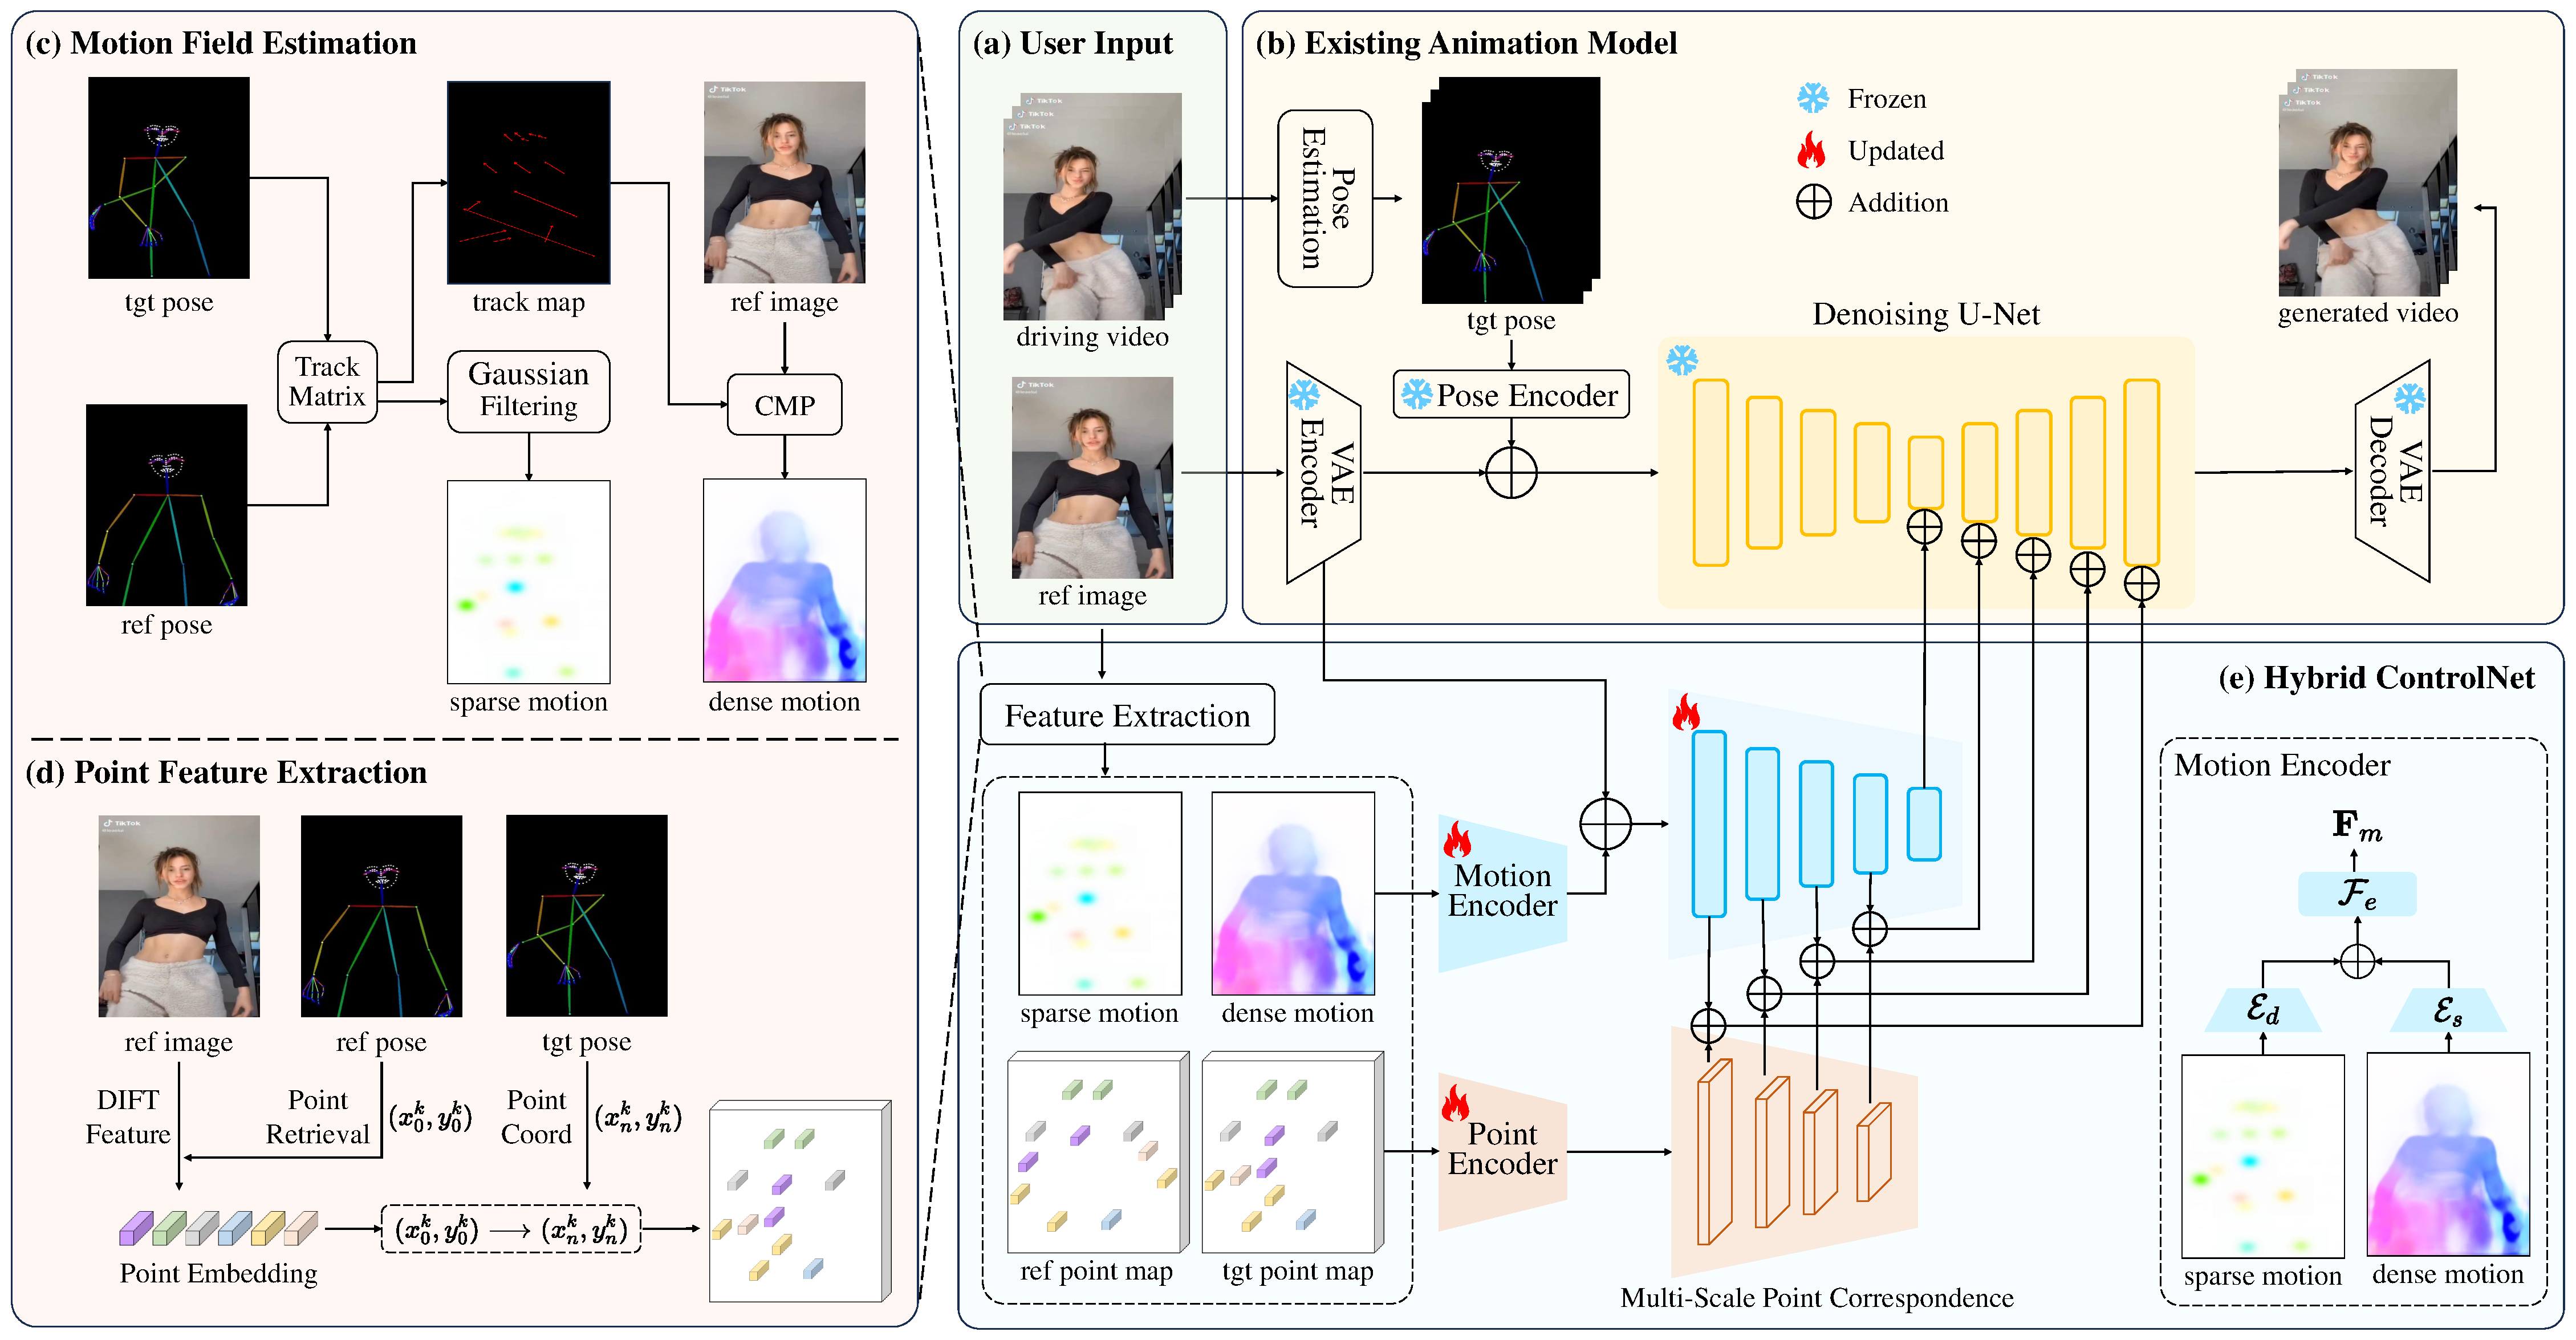
\includegraphics[width=1.0\columnwidth]{./image/pipeline.pdf}
    \vspace{-15pt}
    \caption{The overview of proposed DisPose.}
    \label{fig:pipeline}
\end{figure}
\section{DisPose}
Given a reference image $I_{\mathrm{ref}}\!\in\!\mathbb{R}^{3 \times H \times W}$ and a driving video $V\!\in\!\mathbb{R}^{N\times 3 \times H \times W}$. The core of our method is to disentangle efficient control guidance from only skeleton poses and reference images as shown in Figure~\ref{fig:pipeline}, which can be applied to existing human animation methods without additional dense inputs. We first introduce sparse and dense motion field guides in Sec.~\ref{sec: motion}. Then, we introduce reference-based keypoint correspondence in Sec.~\ref{sec: keypoint}. Finally, we introduce the pipeline of hybrid ControlNet in Sec~\ref{sec: controlnet}.
\subsection{Motion Field Guidance}
\label{sec: motion}

\textbf{Sparse Motion Field.}
We first estimate the skeleton pose by DWpose~\citep{yang2023dwpose} to obtain each frame's human key point coordinates. 
% Subsequently, the motion trajectory of all semantic points in the entire video is obtained and represented as
Subsequently, the key points of the reference image are used as starting points to track the motion displacement of all frames and represented as $P_{traj}\!=\!\{(x^k_n,y^k_n) \!\mid\! k=1\dots K, n=0\dots N\}$, where $P_{traj}$ denotes the trajectory map of the key point $k$ overall $N$ frames and $n = 0$ denotes the reference image. We calculate the track matrix $P_{s}$ as follows:
\begin{equation}
    \mathbf{P}_{s}=\{(x^k_n-x^k_{n-1}, y^k_n-y^k_{n-1}) \mid n=1\dots N\}\},
\end{equation}
% where $P_{t}$ denotes the trajectory map of the key point point $k$ over all $N$ frames, and the reference frame when $n = 0$.
where $K$ denotes the number of keypoints, $N$ denotes the number of frames, $\mathbf{P}_{s}$ denotes the trajectory map of keypoint k over all N frames, and $n = 0$ denotes the reference image.
To avoid training instability caused by overly sparse trajectory matrice, we then apply Gaussian filtering to enhance $\mathbf{P}_{s}$ to obtain the sparse motion field $\mathbf{F}_s\!\in\!\mathbb{R}^{(N-1)\times 2 \times H \times W}$ inspired by~\citep{yin2023dragnuwa, wang2024motionctrl}.

\textbf{Dense Motion Field.}
Considering that sparse control provides limited guidance and dense control is hard to obtain during inference,
% For the dense motion field, 
we transform dense guidance into the motion propagation from the reference frame to the target pose, instead of the dense signal of the target pose. Specifically, in the inference, we reconstruct the trajectory map $\mathbf{P}_{s}$ as the reference-based sparse optical flow $\mathbf{P}_{d}$ from the reference frame to each target pose as:
\begin{equation}
    \mathbf{P}_{d}=\{(x^k_n-x^k_{0}, y^k_n-y^k_{0}) \mid n=1\dots N\}\},
\end{equation}
We then predicted the reference-based dense motion filed $\mathbf{F}_d\!=\! \text{CMP}(P_{traj}, \mathbf{P}_{d}, I_{ref})\!\in\!\mathbb{R}^{(N-1)\times 2 \times H \times W}$ by condition motion propagation (CMP)~\citep{zhan2019self} based on the sparse optical flow $\mathbf{P}_{d}$ and the reference image $I_{ref}$.
CMP~\citep{zhan2019self} is a self-supervised learning-from-motion model that acquires an image and a sparse motion field and estimates the corresponding dense motion field.
Notably, the dense motion field $\mathbf{F}_d$ of each frame starts with the reference image, which avoids geometric constraints during inference.

To ensure motion estimation accuracy during training, we first extract the forward optical flow from the driving video using existing optical flow estimation models~\citep{teed2020raft, xu2023unifying}. We then use a watershed-based approach~\citep{zhan2019self} to sample the sparse optical flow $\mathbf{P}_{d}$ from the forward optical flow. See Appendix.~\ref{sec: appendix1} for details.

\textbf{Motion Encoder.} To leverage motion field as guidance, we introduce a motion encoder specifically designed for the optional flow, which includes sparse motion encoder $\mathcal{E}_s$, dense motion encoder $\mathcal{E}_d$ and feature fusion layer $\mathcal{F}_e$. $\mathcal{E}_d$ and $\mathcal{E}_s$ have the same structure and are multi-scale convolutional encoders with each stage built by \texttt{Conv-SiLU-ZeroConv}~\citep{zhang2023adding} as the basic block. The feature fusion layer $\mathcal{F}_e$ is a 2D convolution for fusing sparse motion features $\mathcal{E}_s(\mathbf{F}_s)$ and dense motion features $\mathcal{E}_d(\mathbf{F}_d)$. Finally, we compute the motion field guidance $\mathbf{F}_m$:
\begin{equation}
    \mathbf{F}_m = \mathcal{F}_e(\mathcal{E}_s(\mathbf{F}_s)+\mathcal{E}_d(\mathbf{F}_d))
\end{equation}

\subsection{Keypoint Correspondence}
\label{sec: keypoint}
\textbf{Point Feature Extraction.} 
To maintain a consistent appearance, it is crucial to correspond the content of the reference image with the motion trajectory. 
Specifically, we first extract the DIFT~\citep{tang2023emergent} features $\mathbf{D}$ of the reference image using the pre-trained image diffusion model. 

Subsequently, the keypoint embedding in the reference is obtained as $\mathbf{D}(x^k_0,y^k_0)$, where $(x^k_0,y^k_0)$ is retrieved from the reference pose.
% key point embeddings $\mathbf{D}(x^k_0,y^k_0)$ are retrieved from $\mathbf{D}$ by skeleton pose $(x^k_0, y^k_0)$.
Next, we initialize the keypoint correspondence map $\mathbf{F}_p$ with zero vectors and assign point embeddings according to the trajectory coordinates as:
\begin{equation}
\label{eq: v prob}
f^{ij}_n=\left\{\begin{array}{ll}
\mathbf{D}(x^k_0,y^k_0), & \mathrm{if} \quad i=x^k_n, j=y^k_n,  \\
0, & \mathrm{otherwise}.
\end{array}\right.
\end{equation}

Finally, we obtain the keypoint correspondence map $\mathbf{F}_p=\{f_n\!\mid\!n=1\dots N\} \!\in\!\mathbb{R}^{N\times D_p \times H \times W}$ for all frames, where $D_p$ is the feature dimension of the point embedding.

\textbf{Point Encoder.} 
To utilize the content correspondence of key points as guidance, we generate multi-scale correspondences of sparse point feature maps and make them compatible with the U-Net encoder of the {Hybrid ControlNet (Sec.4.3)}. 
% as detailed in F. 1.
We introduce the multi-scale point encoder $\mathcal{E}_p$ to maintain the key point content $\mathbf{F}_p$ from the reference image. The point encoder $\mathcal{E}_p$ consists of a series of learnable MLPs.
{
To seamlessly integrate into existing models, we extract intermediate features of the encoder of the hybrid Controlnet.
The multi-scale intermediate features of the Controlnet encoder are denoted as $\mathbf{E}^l_{enc}$, where $l$ denotes each U-Net block $l\!\in\![1, L]$.}
To match the spatial size of $\mathbf{E}^l_{enc}$, we apply downsampling to the feature map between the encoder layers. We compute the multi-scale keypoint correspondence as follows:
\begin{equation}
    \mathbf{F}_c^l = \mathcal{E}_p^l(\phi(\mathbf{F}_p, H^l, W^l)),
\end{equation}
where $(H^l, W^l)$ are denote the spatial dimension of the $l$-th U-Net block and $\phi$ means downsampling operation. Therefore, $\mathbf{F}_c^l$ shares the same size as $\mathbf{E}^l_{enc}$.
Finally, $\mathbf{F}_c$ are added elementwisely to the intermediate feature $\mathbf{E}^l_{enc}$ of the U-Net encoder as guidance: $\mathbf{E}^l_{enc}\!=\!\mathbf{E}^l_{enc}+\mathbf{F}_c^l$.


\subsection{Plug-and-play Hybrid ControlNet}
\label{sec: controlnet}
After obtaining motion field guidance and keypoint correspondence, we aim to integrate these control guidance seamlessly into the U-Net architecture of existing animation models.
Inspired by ControlNet~\citep{zhang2023adding}, We design a hybrid ControlNet $\mathcal{F}$ to provide additional control signals for the existing animation model as shown in Figure~\ref{fig:pipeline}(e).
% Specifically, we consider freeze denoising U-Net and pose encoder. 
Specifically, given an animation diffusion model based on the U-Net architecture, we freeze all its modules while allowing the motion encoder, point encoder and hybrid ControlNet to be updated during training. 
Subsequently, $\mathbf{F}_m$ is added to the noise latent before being input into the hybrid ControlNet. Considering the high sparsity of the point feature $\mathbf{F}_c$, we correspondingly add $\mathbf{F}_c$ to the input of the convolutional layer. Notably, the U-Net encoder intermediate feature $\mathbf{E}_{enc}$ in Sec.~\ref{sec: keypoint} is from hybrid ControlNet rather than denoising U-Net. Finally, 
the control condition is computed as:
\begin{equation}
    \boldsymbol{r}=\mathcal{F}(\boldsymbol{z}_{{t}} \mid \mathbf{F}_m, \mathbf{F}_c, {t})
\end{equation}
where $\boldsymbol{r}$ is a set of condition residuals added to the residuals for the middle and upsampling blocks in the denoising U-Net.
\section{Experiments}
\label{sec:experiments}

We validate our approach empirically, showing that our Monarch matrix parametrization achieves a favorable efficiency--accuracy tradeoff compared to baselines on a wide range of domains (text, images, PDEs, MRI), in three settings (E2E training, S2D training, and D2S fine-tuning):
\begin{itemize}[leftmargin=*,nosep,nolistsep,noitemsep]
\item
In \cref{subsec:benchmark_tasks}, on image classification and language modeling benchmarks, such as ViT / MLP Mixer on ImageNet and GPT-2 on Wikitext-103, Monarch is 2$\times$ faster to train than dense models, while achieving the same accuracy / perplexity. In \cref{subsec:pde_mri}, in scientific and medical domains where special transforms (Fourier) are common, Monarch outperforms Fourier transform based methods on PDE solving, with up to 40\% lower error, and on MRI reconstruction attains up to 15\% higher pSNR and 3.8\% higher SSIM.
\item In \cref{subsec:pde_mri}, we show that on the large OpenWebText dataset, reverse sparsification (training with Monarch weight matrices for most of the time, then transitioning to dense weight matrices) speeds up the pretraining of GPT-2 models by 2$\times$ compared to the dense model, with no loss in upstream or downstream quality.
Moreover, reverse sparsification speeds up BERT pretraining by 23\% even compared to the implementation from Nvidia that set the MLPerf~\citep{mattson2020mlperf} 1.1 record.
\item In \cref{subsec:finetuning}, as a proof of concept, we demonstrate that our Monarch approximation algorithm can improve fine-tuning efficiency for pretrained models. We show that compressing BERT to a Monarch matrix model performs comparably to a finetuned dense model on GLUE, with 2$\times$ fewer parameters and 1.7$\times$ faster finetuning speed.
\end{itemize}

\subsection{End-to-End Training}
\label{subsec:e2e_training}
\subsubsection{Benchmark Tasks: Image Classification, Language Modeling}
\label{subsec:benchmark_tasks}

We show that replacing dense matrices with Monarch matrices in ViT, MLP-Mixer, and
GPT-2 can speed up training by up to 2$\times$ without sacrificing model quality in~\cref{table:pretrain,table:gpt_pretrain}.

\textbf{Setup.} We use the popular vision benchmark, ImageNet~\citep{deng2009imagenet}. We choose recent popular Vision Transformer~\citep{dosovitskiy2020image}, and MLP-Mixer~\citep{tolstikhin2021mlp} as representative base dense models.
For language modeling, we evaluate GPT-2~\citep{radford2019language} on WikiText-103~\citep{merity2016pointer}.

\begin{table}[h]
  \small
  \centering
  \vspace{-2mm}
  \caption{\label{table:pretrain}The performance of Monarch matrices and ViT / MLP-Mixer on ImageNet, including the number of parameters and FLOPs. We measure the Top-1 accuracy and the training time speedup compared to the corresponding dense model. %
  \vspace{2mm}
  }
  \iftoggle{arxiv}{}{
  \resizebox{\linewidth}{!}
  }
  {
  \setlength{\tabcolsep}{3pt}
  \vspace{3em}
  \begin{tabular}{@{}c||ccccccc@{}}
  \specialrule{.15em}{.05em}{.05em}
    Model&\multicolumn{1}{c}{ImageNet acc.}&\multicolumn{1}{c}{Speedup} &\multicolumn{1}{c}{Params} & \multicolumn{1}{c}{FLOPs} \\
    \specialrule{.15em}{.05em}{.05em}
    Mixer-S/16& 74.0& - & 18.5M & 3.8G \\
    Monarch-Mixer-S/16& 73.7& 1.7$\times$ & 7.0M & 1.5G \\
    Mixer-B/16& 77.7& - & 59.9M & 12.6G \\
    Monarch-Mixer-B/16& 77.8& 1.9$\times$ & 20.9M & 5.0G \\
    \specialrule{.15em}{.05em}{.05em}
    ViT-S/16& 79.4 & - & 48.8M & 9.9G \\
    Monarch-ViT-S/16& 79.1 & 1.9$\times$ & 19.6M & 3.9G \\
    ViT-B/16& 78.5 & - & 86.6M  & 17.6G \\
    Monarch-ViT-B/16& 78.9 & 2.0$\times$ & 33.0M & 5.9G \\
    \specialrule{.15em}{.05em}{.05em}
  \end{tabular}
  }
\end{table}

\begin{table}[h]
  \small
  \centering
  \vspace{-3mm}
  \caption{\label{table:gpt_pretrain} Performance of Monarch matrices and GPT-2-Small/Medium on WikiText-103, including the \# of parameters and FLOPs. Monarch achieves similar perplexity (ppl) but 2.0$\times$ faster.}
  \vspace{1mm}
  \iftoggle{arxiv}{}{
    \resizebox{0.95\linewidth}{!}
  }
  {
\setlength{\tabcolsep}{5pt}
\begin{tabular}{c||cccc}
\specialrule{.15em}{.05em}{.05em}
\multirow{1}{*}{{ Model} } & \multicolumn{1}{c}{\multirow{1}{*}{PPL}}
                              & \multicolumn{1}{c}{\multirow{1}{*}{Speedup}}
                              & \multicolumn{1}{c}{\multirow{1}{*}{Params}}
                              & \multicolumn{1}{c}{\multirow{1}{*}{FLOPs}}\\
\specialrule{.15em}{.05em}{.05em}
GPT-2-Small &  20.6 & - & 124M& 106G\\
Monarch-GPT-2-Small& 20.7  & 1.8$\times$ &72M & 51G\\
\specialrule{.15em}{.05em}{.05em}
GPT-2-Medium &  20.9 & - & 355M& 361G\\
Monarch-GPT-2-Medium& 20.3  & 2.0$\times$ &165M & 166G\\
\specialrule{.15em}{.05em}{.05em}
\end{tabular}
}
\vspace{-2mm}
\end{table}


\subsubsection{PDE solving and multi-coil MRI reconstruction}
\label{subsec:pde_mri}

Many scientific or medical imaging tasks rely on specialized transforms such as the
Fourier transform.
We show that replacing the fixed Fourier transform with the more expressive
Monarch matrices yields higher model quality (lower reconstruction error) with
comparable model speed.

\textbf{Solving PDEs with Monarch Neural Operators.}
We follow the experimental setting in FNO~\citep{li2020fourier} and apply a Monarch--based neural operator to the task of solving the Navier--Stokes PDE. Compared to baseline U-Nets~\citep{ronneberger2015u}, TF-Nets~\citep{wang2020towards}, ResNets~\citep{he2016deep} and FNOs~\cite{li2020fourier}, neural operators based on Monarch improve solution accuracy across spatial resolutions by up to $40\%$ (Table \ref{table:pde}).  





\paragraph{Non-periodic boundary conditions.} Traditional spectral methods based on Fourier transform work best with periodic boundary conditions and forcing terms. However, PDEs of practical interest often exhibit non--periodic or even unknown boundary conditions. Monarch operators are not constrained to the Fourier transform and can thus still learn the solution operator with excellent accuracy.

\begin{table}[h!] 
\scriptsize
\vspace{-4mm}
\caption{\label{table:pde}Benchmarks on Navier-Stokes (fixing resolution 64 × 64 for both training and testing).
Decreasing the viscosity coefficient $\nu$ makes the dynamics more chaotic.
}
\vspace{1mm}
\centering
\iftoggle{arxiv}{}{
  \resizebox{0.9\linewidth}{!}
}
{
\renewcommand{\arraystretch}{1}
\begin{tabular}{ c||ccc }
\specialrule{.15em}{.05em}{.05em}
Model & $v = 10^{-3}$  &  $v = 10^{-4}$ & $v = 10^{-5}$\\
\specialrule{.15em}{.05em}{.05em}
U-Net & 0.025  & 0.205  &   0.198\\
TF-Net  & 0.023  & 0.225 &  0.227 \\
ResNet & 0.070 &  0.287 &  0.275 \\
FNO & 0.017  & 0.178 & 0.155\\
Monarch-NO & \textbf{0.010} & \textbf{0.145} & \textbf{0.136} \\
\specialrule{.15em}{.05em}{.05em}
\end{tabular}
}
\textbf{\vspace{-3mm}}
\end{table}

\textbf{Accelerated MRI Reconstruction.} We characterize the utility of Monarch-based FFT operations for accelerated MRI reconstruction, a task which requires methods with both structured Fourier operators and dealiasing properties to recover high quality images. On the clinically-acquired 3D MRI SKM-TEA dataset \citep{desai2021skm}, Monarch-SENSE (mSENSE) enhances image quality by over 1.5dB pSNR and 2.5\% SSIM compared to zero-filled SENSE and up to 4.4dB and 3.8\% SSIM compared to U-Net baselines in data-limited settings. Setup details are available in~\cref{sec:experiment_details_mri}.

\paragraph{Expressive FFT.} By definition, standard IFFT in zero-filled SENSE cannot dealias the signal, resulting in artifacts in the reconstructed image. mSENSE replaces the inverse FFT (IFFT) operation in standard SENSE with learnable Monarch matrices. Thus, mSENSE preserves the structure of the Fourier transform while learning to reweight frequencies to suppress aliasing artifacts. Across multiple accelerations, mSENSE achieved up to +1.5dB and 2.5\% improvement in peak signal-to-noise ratio (pSNR) and structural similarity (SSIM), respectively (Table~\ref{table:mri}).

\paragraph{Data Efficiency.} While CNNs have shown promise for MRI reconstruction tasks, training these networks requires extensive amounts of labeled data to avoid overfitting. However, large data corpora are difficult to acquire in practice. mSENSE can be trained efficiently with limited supervised examples. In few shot settings, mSENSE can outperform U-Net by +4.4dB ($\approx$15\%) and 3.8\% SSIM (Table~\ref{table:mri-data-limited}). 







\begin{table}[h!] 
\scriptsize
\vspace{-3mm}
\caption{\label{table:mri}Mean $\pm$ standard error of the mean of conventional and Monarch-SENSE (mSENSE) on dual-echo (E1,E2) MRI reconstruction at multiple acceleration factors (Acc.).
}
\vspace{1mm}
\centering
\iftoggle{arxiv}{}{
  \resizebox{\linewidth}{!}
}
{
\renewcommand{\arraystretch}{1.2}
\begin{tabular}{c||ccccc}
\specialrule{.15em}{.05em}{.05em}
  & & \multicolumn{2}{c}{pSNR (dB) ($\uparrow$)} & \multicolumn{2}{c}{SSIM ($\uparrow$)} \\
  Acc. & Model &             E1 &             E2 &                E1 &                E2 \\
\specialrule{.15em}{.05em}{.05em}
\multirow{2}{*}{2} & SENSE &  32.8$\pm$0.2 &  35.4$\pm$0.2 &  0.871$\pm$0.003 &  0.865$\pm$0.003 \\
  & mSENSE &  \textbf{34.3$\pm$0.2} &  \textbf{36.6$\pm$0.2} &  \textbf{0.886$\pm$0.002} &  \textbf{0.882$\pm$0.003} \\
\specialrule{.15em}{.05em}{.05em}
\multirow{2}{*}{3} & SENSE &  30.9$\pm$0.2 &  33.5$\pm$0.2 &  0.819$\pm$0.004 &  0.795$\pm$0.004 \\
  & mSENSE &  \textbf{32.3$\pm$0.2} &  \textbf{34.6$\pm$0.2} &  \textbf{0.843$\pm$0.003} &  \textbf{0.820$\pm$0.004} \\
\specialrule{.15em}{.05em}{.05em}
\multirow{2}{*}{4} & SENSE &  30.1$\pm$0.2 &  32.8$\pm$0.2 &  0.789$\pm$0.004 &  0.753$\pm$0.005 \\
  & mSENSE &  \textbf{31.2$\pm$0.2} &  \textbf{33.5$\pm$0.2} &  \textbf{0.812$\pm$0.003} &  \textbf{0.767$\pm$0.005} \\
\specialrule{.15em}{.05em}{.05em}
\end{tabular}
}
\end{table}

\begin{table}[h!] 
\scriptsize
\vspace{-5mm}
\caption{\label{table:mri-data-limited}Impact of number of training examples ($N$) on dual-echo MRI reconstruction at 2x acceleration.
}
\vspace{1mm}
\centering
\iftoggle{arxiv}{}{
  \resizebox{\linewidth}{!}
}
{
\renewcommand{\arraystretch}{1.2}
\begin{tabular}{c||ccccc}
\specialrule{.15em}{.05em}{.05em}
  &  & \multicolumn{2}{c}{pSNR (dB) ($\uparrow$)} & \multicolumn{2}{c}{SSIM ($\uparrow$)} \\
  $N$ & Model &            E1 &            E2 &               E1 &               E2 \\
\specialrule{.15em}{.05em}{.05em}
N/A & SENSE &  32.8$\pm$0.2 &  35.4$\pm$0.2 &  0.871$\pm$0.003 &  0.865$\pm$0.003 \\
\specialrule{.15em}{.05em}{.05em}
\multirow{2}{*}{1} & U-Net &  29.4$\pm$0.2 &  34.4$\pm$0.3 &  0.848$\pm$0.004 &  0.857$\pm$0.004 \\
  & mSENSE &  \textbf{33.8$\pm$0.2} &  \textbf{36.0$\pm$0.2} &  \textbf{0.886$\pm$0.003} &  \textbf{0.867$\pm$0.003} \\
\specialrule{.15em}{.05em}{.05em}
\multirow{2}{*}{2} & U-Net &  29.9$\pm$0.3 &  35.1$\pm$0.3 &  0.858$\pm$0.003 &  0.871$\pm$0.003 \\
  & mSENSE &  \textbf{34.0$\pm$0.2} &  \textbf{36.4$\pm$0.2} &  \textbf{0.883$\pm$0.002} &  \textbf{0.877$\pm$0.003} \\
\specialrule{.15em}{.05em}{.05em}
\multirow{2}{*}{3} & U-Net &  31.0$\pm$0.3 &  35.2$\pm$0.3 &  0.866$\pm$0.003 &  0.867$\pm$0.004 \\
  & mSENSE &  \textbf{33.9$\pm$0.2} & \textbf{ 36.5$\pm$0.2} &  \textbf{0.882$\pm$0.002} & \textbf{0.878$\pm$0.003} \\
\specialrule{.15em}{.05em}{.05em}
\multirow{2}{*}{5} & U-Net &  31.4$\pm$0.3 &  35.6$\pm$0.2 &  0.877$\pm$0.002 &  0.870$\pm$0.003 \\
  & mSENSE &  \textbf{33.9$\pm$0.2} &  \textbf{36.5$\pm$0.2} &  \textbf{0.881$\pm$0.002} &  \textbf{0.877$\pm$0.003} \\
\specialrule{.15em}{.05em}{.05em}
\end{tabular}
}
\end{table}




\subsection{Sparse-to-Dense Training (reverse sparsification)}
\label{subsec:s2d_training}
\paragraph{GPT-2 pretraining.}
On the large OpenWebtext dataset~\citep{Gokaslan2019OpenWeb}, we train a GPT-2 model with Monarch weight
matrices for 90\% of the training iterations, then relax the constraint on the
weight matrices and train them as dense matrices for the remaining 10\% of the
iterations.
We call this technique ``reverse sparsification.''
Previous sparse training techniques often don't speed up training, whereas our
hardware-efficient Monarch matrices do.
Therefore we can use them as an intermediate step to pretrain a large language
model (GPT-2) in 2$\times$ less time. We also evaluate its downstream quality on zero-shot generation from~\citep{eval-harness} and classification tasks from~\citep{zhao2021calibrate}, achieving comparable performance to the dense counterparts (\cref{table:gpt_finetune}). 

\begin{table}[h]
  \small
  \centering
  \vspace{-3mm}
  \caption{\label{table:gpt_finetune}The performance (accuracy) of GPT-2-medium trained with Monarch reverse sparsification and with conventional dense training on text classification benchmarks.}
  \setlength{\tabcolsep}{5pt}
  \vspace{1em}
  \iftoggle{arxiv}{}{
    \resizebox{\linewidth}{!}
  }
  {
  \begin{tabular}{@{}c||ccc@{}}
    \specialrule{.15em}{.05em}{.05em}
    Model&\multicolumn{1}{c}{OpenWebText (ppl)}&\multicolumn{1}{c}{Speedup}& \multicolumn{1}{c}{Classification (avg acc)} \\
    \specialrule{.15em}{.05em}{.05em}
    GPT-2m& 18.0 & - & 38.9 \\
    Monarch-GPT-2m& 18.0 & 2$\times$ & 38.8 \\
    \specialrule{.15em}{.05em}{.05em}
  \end{tabular}
  }
  \vspace{-3mm}
\end{table}


In \cref{fig:reverse_sparsification_bar}, we show the training time of the dense GPT-2 model, along with
the Monarch GPT-2 model.
After training the Monarch model for 90\% of the time, in the
last 10\% of the training steps, by transitioning to dense weight matrices, the model is able to reach the same 
performance of another model that was trained with dense weight matrices from
scratch.
By training with Monarch matrices for 90\% of the time, we reduce the total training time by 2$\times$.

\paragraph{BERT pretraining.}
On the Wikipedia + BookCorpus datasets~\citep{zhu2015aligning}, we train a BERT-large model with Monarch weight matrices for 70\% of the time and transition to dense weight matrices for the remaining 30\% of the time, which yields the same pretraining loss as conventional dense training.
In \cref{table:bert_speed}, we compare the total training time to several baseline implementations: the widely-used implementation from HuggingFace~\citep{wolf-etal-2020-transformers}, the more optimized implementation from Megatron~\citep{shoeybi2019megatron}, and the most optimized implementation we know of from Nvidia that was used to set MLPerf 1.1 training speed record. Our method is 3.5x faster than HuggingFace and 23\% faster than Nvidia's MLPerf 1.1 implementation\footnote{Our result is not an official MLPerf submission. We train BERT for both phase 1 (sequence length 128) and phase 2 (sequence length 512) according to the standard BERT training recipe\cite{devlin2018bert}, while MLPerf only measures training time for phase 2.}.
Experiment details are in~\cref{subsec:bert_details}.

\begin{table}[h]
  \small
  \centering
  \caption{\label{table:bert_speed}The total training time of BERT-large trained with Monarch reverse sparsification and with conventional dense training on 8 A100-40GB GPUs (DGX A100). Training consists of two phases, phase 1 with sequence length 128 and phase 2 with sequence length 512. Monarch training is 3.5x faster than HuggingFace and 23\% faster than Nvidia's MLPerf 1.1 implementation.}
  \vspace{1em}
  \iftoggle{arxiv}{}{
    \resizebox{\linewidth}{!}
  }
  {
    \begin{tabular}{@{}c||c@{}}
      Implementation & Training time (h)  \\ \hline
      HuggingFace &  84.5 \\
      MegaTron & 52.5 \\
      Nvidia MLPerf 1.1 & 30.2 \\
      Nvidia MLPerf 1.1 + DeepSpeed & 29.3 \\
      Monarch (ours) & \textbf{23.8} \\
    \end{tabular}
  }
  \vspace{-3mm}
\end{table}

\subsection{Dense-to-Sparse Fine-tuning}
\label{subsec:finetuning}

\begin{figure}[t]
  \centering
  \vspace{-3mm}
  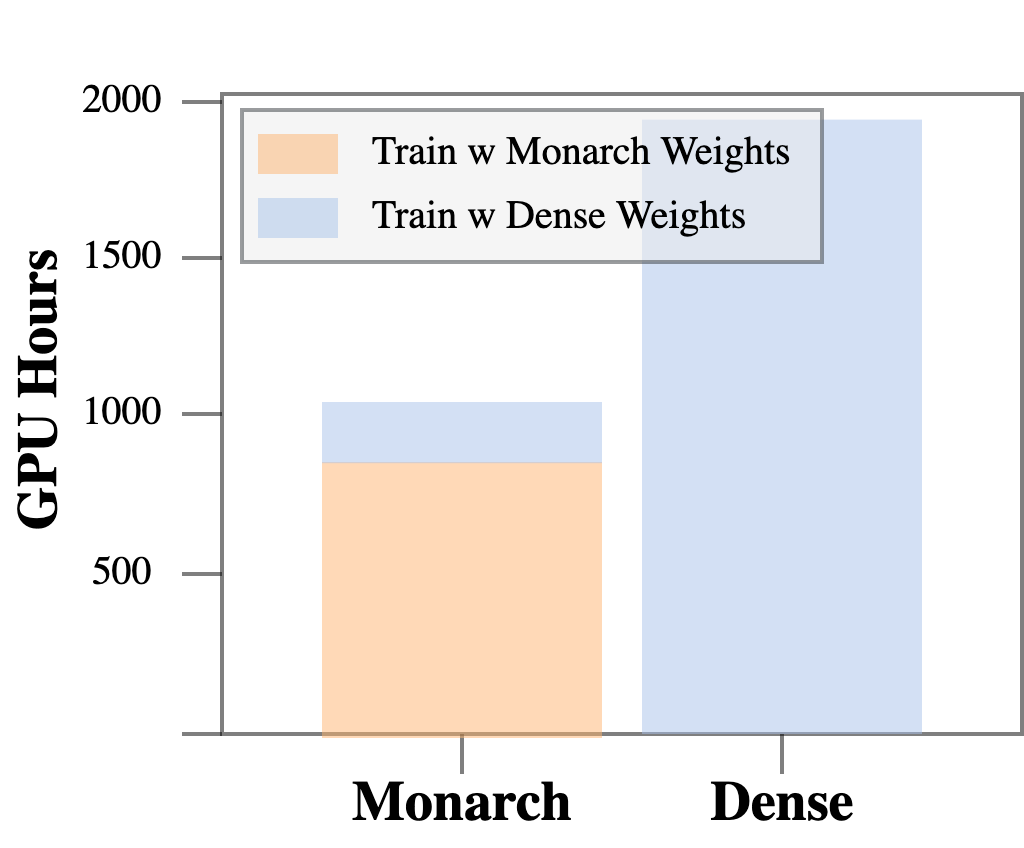
\includegraphics[width=.3\textwidth]{figures/rv_bar_temp.png}
  \vspace{-3mm}
  \caption{\label{fig:reverse_sparsification_bar}Time required (in A100 GPU hours) to reach the same perplexity (18.0)
    for GPT-2-small on OpenWebText.
    With ``reverse sparsification'', Monarch can speed up
    GPT-2 training by 2$\times$.\vspace{-1em}}
\end{figure}

We show that our Monarch approximation algorithm allows us to efficiently use
pretrained models, such as speeding up BERT finetuning on GLUE.

\paragraph{BERT finetuning.}
We take the BERT pretrained weights, approximate them with Monarch matrices,
and finetune the resulting model on the 9 GLUE tasks.
The results in \cref{table:bert_glue} shows that we obtain a Monarch finetuned
model with similar quality to the dense BERT model, but with 1.7$\times$ faster
finetuning speed.
This serves as a proof of concept, and we expect further speedup if additional model compression techniques are applied (e.g., quantization, kernel fusion).




\begin{table}[h]
  \small
  \centering
  \vspace{-5mm}
  \caption{\label{table:bert_glue}The performance of Monarch matrices in
    finetuning BERT on GLUE.}
  \setlength{\tabcolsep}{5pt}
  \vspace{1em}
  \iftoggle{arxiv}{}{
    \resizebox{\linewidth}{!}
  }
  {
  \begin{tabular}{@{}c||ccccccc@{}}
  \specialrule{.15em}{.05em}{.05em}
    Model&\multicolumn{1}{c}{GLUE (avg)}&\multicolumn{1}{c}{Speedup} &\multicolumn{1}{c}{Params} & \multicolumn{1}{c}{FLOPs} \\
    \specialrule{.15em}{.05em}{.05em}
    BERT-base & 78.6& - & 109M & 11.2G \\
    Monarch-BERT-base& 78.3& 1.5$\times$ & 55M & 6.2G  \\
    BERT-large & 80.4 & - & 335M & 39.5G \\
    Monarch-BERT-large & 79.6 & 1.7$\times$ & 144M & 14.6G  \\
    \specialrule{.15em}{.05em}{.05em}
  \end{tabular}
  }
  \vspace{-3mm}
\end{table}



\bibliography{icml/medusa_icml}
\bibliographystyle{icml2024}


\newpage
\appendix
\onecolumn
\section{Related Work}
\label{section:related_work}
The development of Llama 3 builds on a large body of prior work studying foundation models for language, images, videos, and speech.
A comprehensive overview of that work is outside the scope of this paper; we refer the reader to \citet{bordes2024vlm,madan2024foundation,LLMSurvey} for such overviews.
Below, we briefly outline seminal works that directly influenced the development of Llama 3.

\subsection{Language}
\label{section:related_work_language}

\textbf{Scale.}
Llama 3 follows the enduring trend of applying straightforward methods at ever increasing scales in foundation models. Improvements are driven by increased compute and improved data, with the 405B model using almost fifty times the pre-training compute budget of Llama 2 70B. Despite containing 405B parameters, our largest Llama 3 in fact contains fewer parameters than earlier and much less performant models such as PALM~\citep{chowdhery2023palm}, due to better understanding of scaling laws~\citep{kaplan2020scaling,hoffmann2022chinchilla}. Little is publicly known about the size of other frontier models, such as Claude 3 or GPT 4~\citep{openai2023gpt4}, but overall performance is compareable. 

\textbf{Small models.}
Developments in smaller models have paralleled those in large models. 
Models with fewer parameters can dramatically improve inference cost and simplify deployment~\citep{mehta2024openelm,team2024gemma}.
The smaller Llama 3 models achieve this by training far beyond the point of compute optimal training, effectively trading training compute for inference efficiency.
An alternative path is to distill larger models into smaller ones, as in Phi~\citep{abdin2024phi}.

\textbf{Architectures.}
While Llama 3 makes minimal architectural modifiations to compared to Llama 2, other recent foundation models have explored other designs. Most notably, mixture of experts architectures~\citep{shazeer2017moe,lewis2021base,fedus2022switch,zhou2022mixture} can be used as an efficient way to increase the capacity of a models, such as in Mixtral~\citep{jiang2024mixtral} and Arctic~\citep{snowflakearctic}. Llama 3 outperforms these models, suggesting that dense architectures are not the limiting factor, but there remain numerous trade offs in terms of training and inference efficiency, and model stability at scale.

\textbf{Open source.}
Open weights foundation models have rapidly improved over the last year, with Llama3-405B now competitive with the current closed weight state-of-the-art. 
Numerous model families have recently been developed, including Mistral~\citep{jiang2023mistral}, Falcon~\citep{almazrouei2023falcon}, MPT~\citep{databricksmpt}, Pythia~\citep{biderman2023pythia}, Arctic~\citep{snowflakearctic}, OpenELM~\citep{mehta2024openelm}, OLMo~\citep{groeneveld2024olmoacceleratingsciencelanguage}, StableLM~\citep{bellagente2024stable}, OpenLLaMA~\citep{openlm2023openllama}, Qwen~\citep{bai2023qwen}, Gemma~\citep{team2024gemma}, Grok~\citep{xaigrok}, and Phi~\citep{abdin2024phi}.

\textbf{Post-training.}
Post-training \llamathree follows the established strategy of instruction tuning~\citep{chung2022scalinginstruction,ouyang2022instructgpt} followed by alignment with human feedback~\citep{kaufmann2023survey}. While some studies have shown the surprising effectiveness of lightweight alignment procedures~\citep{zhou2024lima}, \llamathree uses millions of human instructions and preference judgments to improve the pre-trained model, including techniques such as rejection sampling~\citep{constitutional-ai-bai}, supervised finetuning~\citep{sanh2022multitask}, and Direct Preference Optimization~\citep{rafailov2023dpo}. In order to curate these instruction and preference examples, we deploy earlier versions of \llamathree to filter~\citep{liu2024makesgooddataalignment}, re-write~\citep{pan2024selfcorrection}, or generate prompts and responses~\citep{liu2024bestpractices} and apply these techniques through multiple rounds of post-training.


\subsection{Multimodality}
\label{section:related_work_multimodality}
Our experiments with multimodal capabilities for Llama 3 are part of a long line of work on foundation models that jointly model multiple modalities.

\textbf{Images.} 
A substantial body of work has trained image-recognition models on large amounts of image-text pairs, for example, \citet{Mahajan_2018_ECCV,xiao2024florence,chameleon2024,openai2023gpt4blog}.
\citet{radford2021learning} presented one of the first models to jointly embed images and text via contrastive learning. 
More recently, a series of models has studied approaches similar to the one used in Llama 3, for example, \citet{alayrac2022flamingo,dai2023instructblip,liu2023llava,liu2023improvedllava,yang2023mmreact,ye2023mplug,zhu2023minigpt}.
Our approach in Llama 3 combines ideas from many of these papers to achieve results that are comparable with Gemini 1.0 Ultra \citep{gemini2023gemini} and GPT-4 Vision \citep{openai2023gpt4blog}; see Section~\ref{section:results_image_recognition}.


\textbf{Video.}
Although video inputs are supported by an increasing number of foundation models \citep{gemini2023gemini,openai2023gpt4blog}, the body of work on joint modeling of videos and language is not that large.
Akin to Llama 3, most current studies adopt an adapter approach to align video and language representations and unlock question-answering and reasoning about videos \citep{lin2023video,li2023videochat,Maaz2023VideoChatGPT,zhang2023videollama,zhao2022lavila}.
We find that such approaches produce results that are competitive with the state-of-the-art; see Section~\ref{section:results_video_recognition}.

\textbf{Speech.}
Our work also fits in a larger body of work combining language and speech modeling.
Earlier joint models of text and speech include AudioPaLM \citep{rubenstein2023audiopalm}, VioLA \citep{wang2023viola}, VoxtLM \cite{maiti2023voxtlm}, SUTLM \citep{chou2023sutlm}, and Spirit-LM \citep{nguyen2024spirit}.
Our work builds on prior compositional approaches to combining speech and language like \citet{fathullah2024audiochatllama}.
Unlike most prior work, we opt to not finetune the language model itself for speech tasks as doing so may lead to contention on non-speech tasks.
We find that at larger model scales, strong performances are attainable even without such finetuning; see Section~\ref{section:results_speech}.



\section{Experiment Settings}\label{appendix:experiment_settings}
\subsection{Common Terms}
We clarify three commonly used terms:
a) Acceleration rate: This refers to the average number of tokens decoded per decoding step. In a standard auto-regressive model, this rate is 1.0.
b) Overhead: This is used to characterize the per decoding step overhead compared to classic decoding, and is calculated by dividing the average per step latency of the \ours models by that of the vanilla model.
c) Speedup: This refers to the wall-time acceleration rate. 
Following these definitions, we have the relation: Speedup = Acceleration rate / Overhead.
\subsection{Shared Settings} 
For all the experiments, we use the Axolotl~\citep{axolotl2023} framework for training. We use a cosine learning rate scheduler with warmup and use 8-bit AdamW~\citep{dettmers20218bit} optimizer. We train $5$ \ours heads with $1$ layer and set $\lambda_k$ in Eq.~\eqref{eq:loss_medusa_1} to be $0.8^k$. For \ours-2, we use either LoRA~\citep{hu2021lora} or QLoRA~\citep{dettmers2023qlora} for fine-tuning and set the learning rate of \ours heads to be $4$ times larger than the backbone model. LoRA is applied to all the linear layers of the backbone model, including the language model head. The rank of LoRA adapter is set to $32$, and $\alpha$ is set to $16$. A dropout of $0.05$ is added to the LoRA adapter. 

\subsection{\ours-1 v.s. \ours-2 on Vicuna 7B and 13B} 
We use a global batch size of $64$ and a peak learning rate of $5e^{-4}$ for the backbone and $2e^{-3}$ for \ours heads and warmup for $40$ steps. We use $4$-bit quantized backbone models for both models. We first train the models with \ours-1 and use these trained models as initialization to train \ours-2. We employ QLoRA for \ours-2 and the  $\lambda_0$ in Eq.~\eqref{eq:loss_medusa_2} is set to be $0.2$.
\subsection{ Training with Self-Distillation on Vicuna-33B and Zephyr-7B} 
We use \ours-2 for both models instead of using a two-stage training procedure. We use a sine schedule for the $\theta_0$ to gradually increase the value to its peak at the end of the training. We find this approach is equally effective. We set the peak learning rate of the backbone LoRA adapter to be $1e^{-4}$ and the warmup steps to be $20$ since the self-distillation loss is relatively small. We set the $\lambda_0$ in Eq.~\eqref{eq:loss_medusa_2} to be $0.01$.
\section{Visualization of optimized tree attention}\label{appendix:sparse_tree}
Fig.~\ref{fig:sparse_tree} illustrates the structure of a sparsely constructed tree for the \ours-2 Vicuna-7B model. This tree structure extends four levels deep, indicating the engagement of four \ours heads in the computation. The tree is initially formed through a Cartesian product approach and subsequently refined by pruning based on the statistical expectations of the top-k predictions from each \ours head measured on the Alpaca-eval dataset~\cite{dubois2023alpacafarm}. The tree's lean towards the left visually represents the algorithm's preference for nodes with higher probabilities on each head.
\begin{figure*}[h]
    \centering
    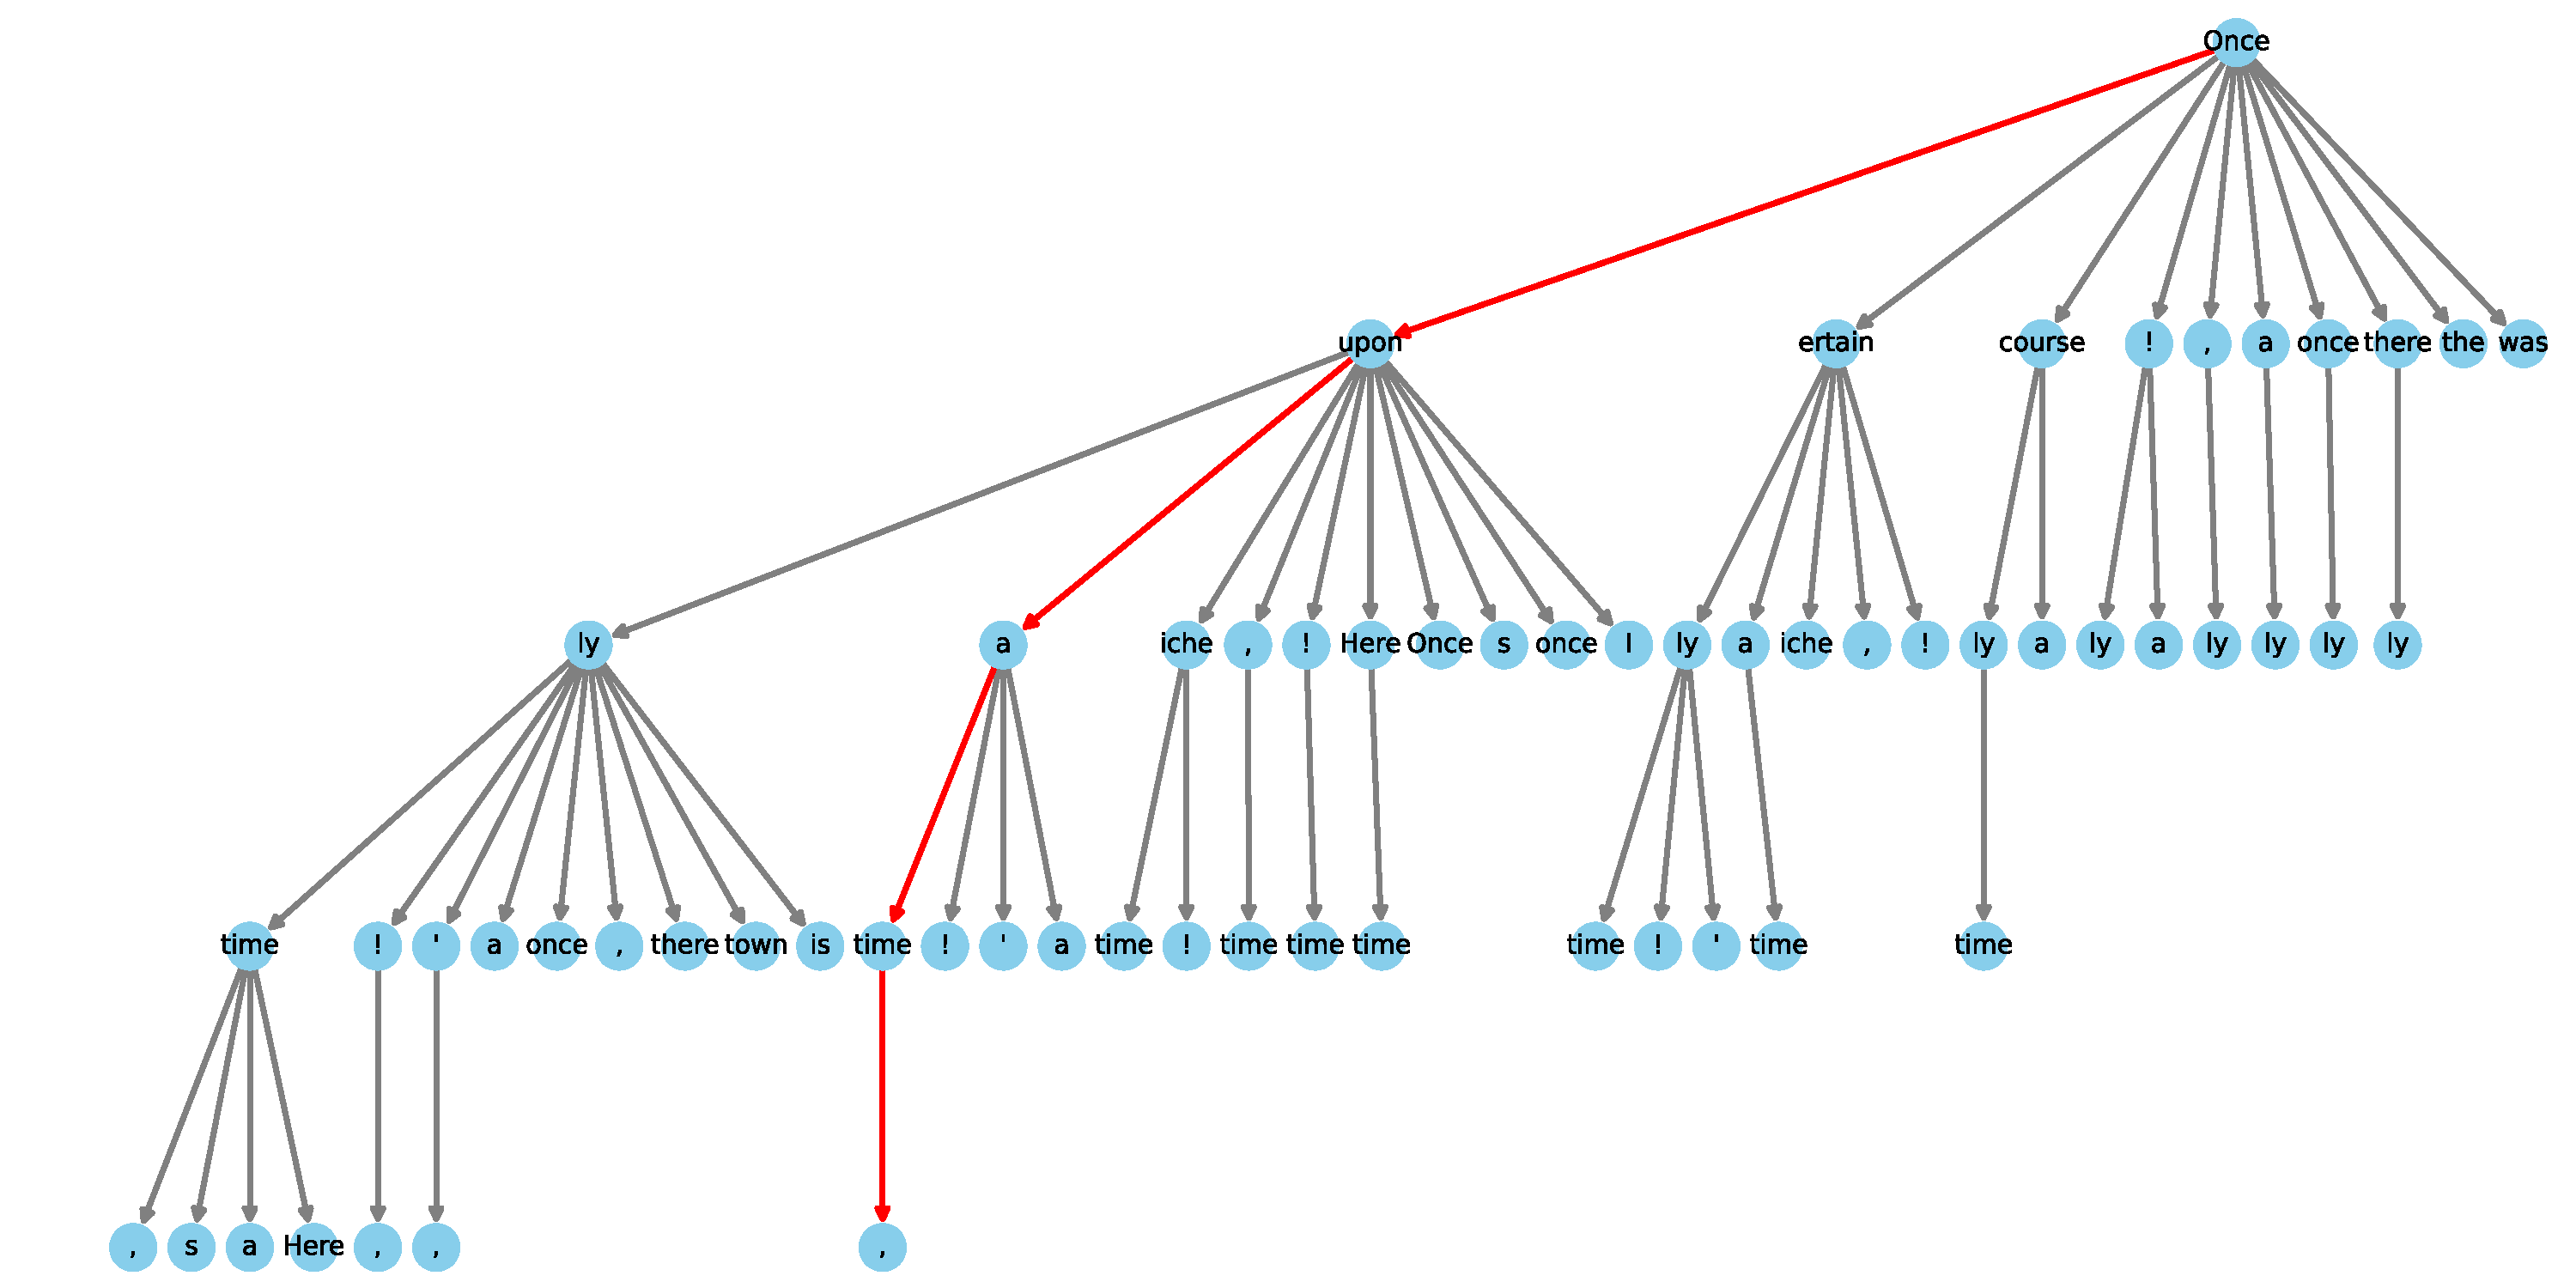
\includegraphics[width=0.6\textwidth]{sparse_tree.pdf}
    \caption{Visualization of a sparse tree setting for \ours-2 Vicuna-7B. The tree has \textcolor{black}{64 nodes representing candidate tokens} and a depth of 4 which indicates 4 \ours heads involved in calculation. Each node indicates a token from a top-k prediction of a \ours head, and the edges show the connections between them. The red lines highlight the path that correctly predicts the future tokens.}
    \label{fig:sparse_tree}
\end{figure*}

\section{Results of Speculative Decoding}\label{appendix:spec}

In this study, speculative decoding was applied to Vicuna models~\citep{vicuna2023} with varying sizes, specifically 7B, 13B, and 33B. The preliminary framework utilized open-source models such as Llama-68M and 160M~\citep{miao2023specinfer}, alongside Tiny-Llama~\citep{zhang2024tinyllama} and Tiny-Vicuna~\citep{tiny_vicuna_1b}, fine-tuned from Tiny-Llama with the Vicuna-style instructional tuning strategy. Due to the proprietary nature of speculative decoding methods~\citep{chen2023accelerating, leviathan2022fast}, open-source alternatives\footnote{\href{https://github.com/feifeibear/LLMSpeculativeSampling}{https://github.com/feifeibear/LLMSpeculativeSampling}} were deployed for evaluation. Additionally, we utilize \verb|torch.compile()| to accelerate the inference speed of draft models.

Our results shown in Fig.~\ref{fig:speculative_decoding}, reveal that the optimal settings of the draft model vary with the Vicuna model sizes. Specifically, the Llama-68M, with a setting of the draft token number $\gamma=4$, yielded the best performance for Vicuna-7B, while the same draft model with $\gamma=3$ was most effective for Vicuna-13B. For the larger Vicuna-33B, the Tiny-Vicuna \textcolor{black}{(Vicuna-1B)}, with $\gamma=3$, provided the greatest acceleration. These results suggest that the choice and setting of the drafting model should be tailored to the size of the LLMs, presenting an area for further exploration in the field.



\begin{figure*}[h]
     \centering
     \begin{subfigure}[b]{0.32\textwidth}
         \centering
         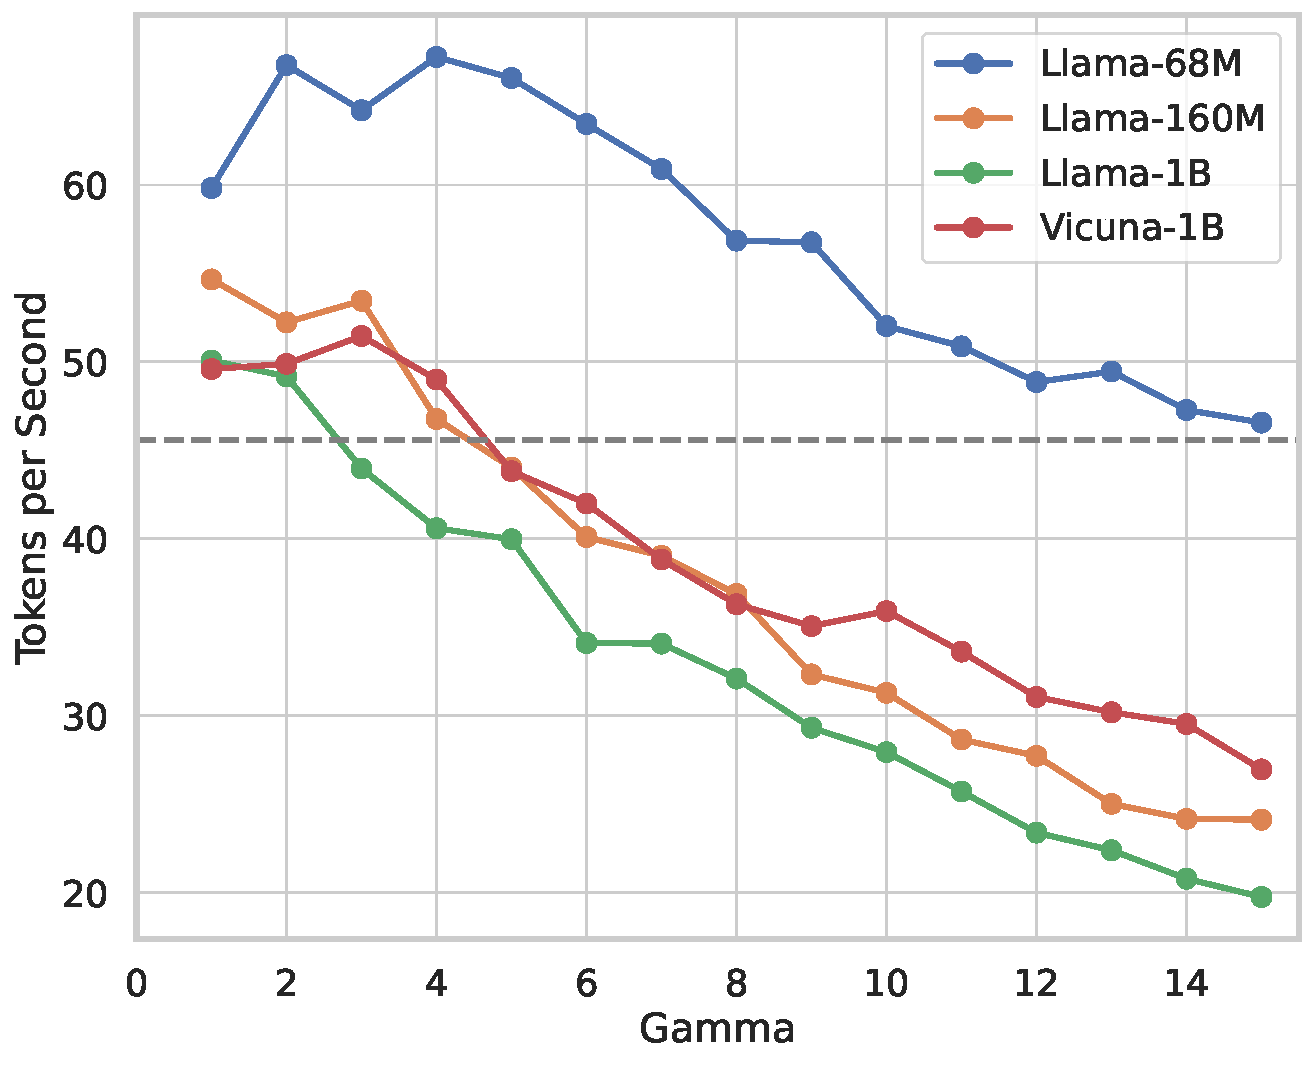
\includegraphics[width=\textwidth]{spec_7b.pdf}
         \caption{Vicuna-7B}
         \label{fig:spec7b}
     \end{subfigure}
     \begin{subfigure}[b]{0.32\textwidth}
         \centering
         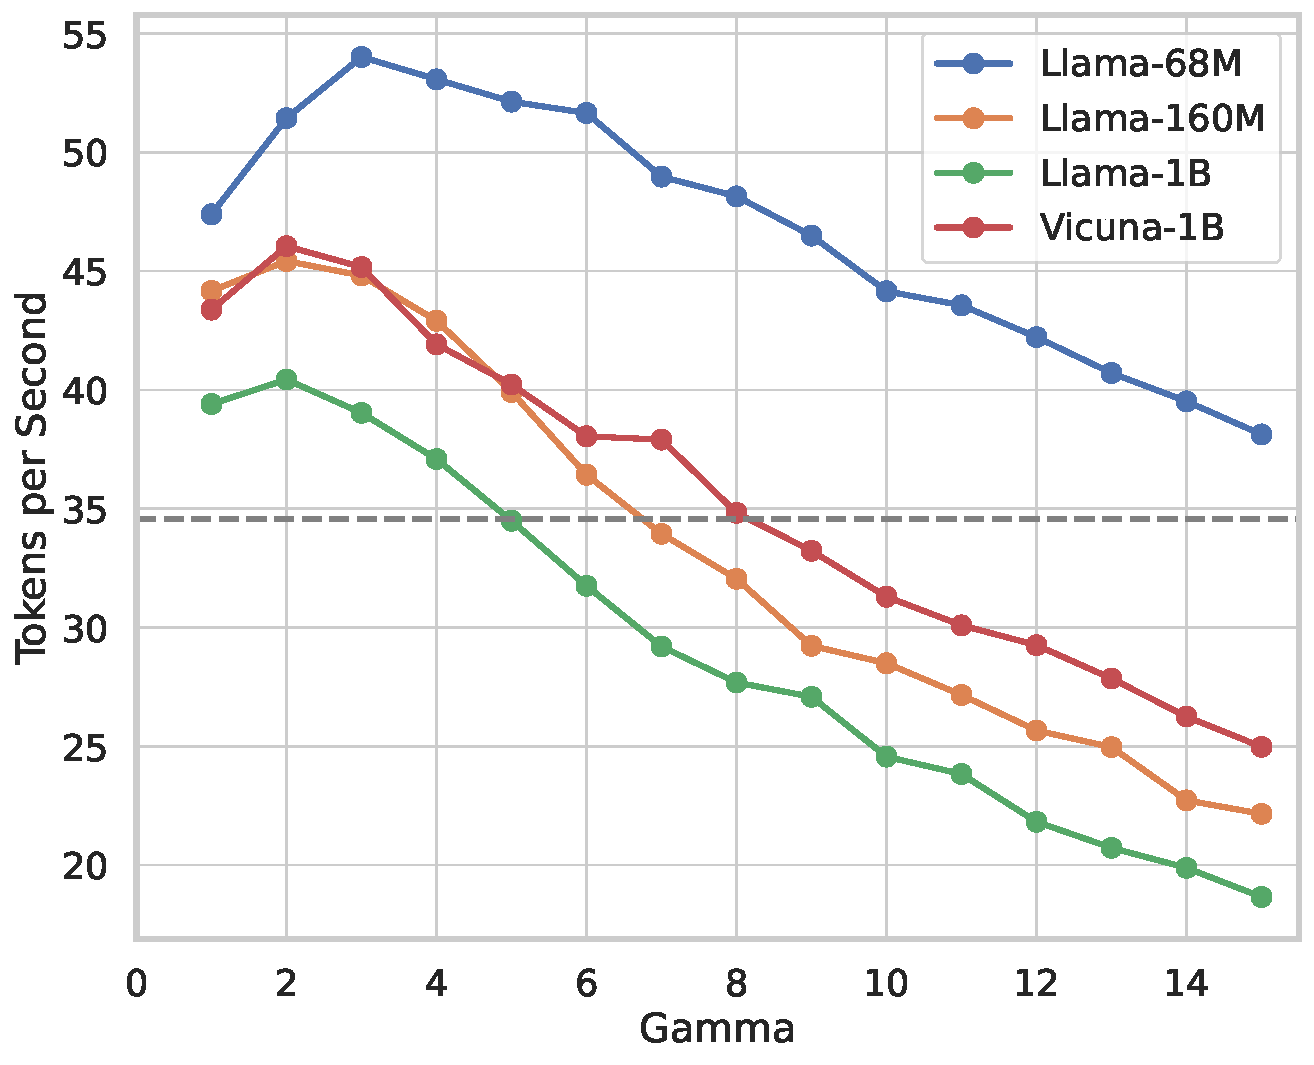
\includegraphics[width=\textwidth]{spec_13b.pdf}
         \caption{Vicuna-13B}
         \label{fig:spec13b}
     \end{subfigure}
    \begin{subfigure}[b]{0.32\textwidth}
         \centering
         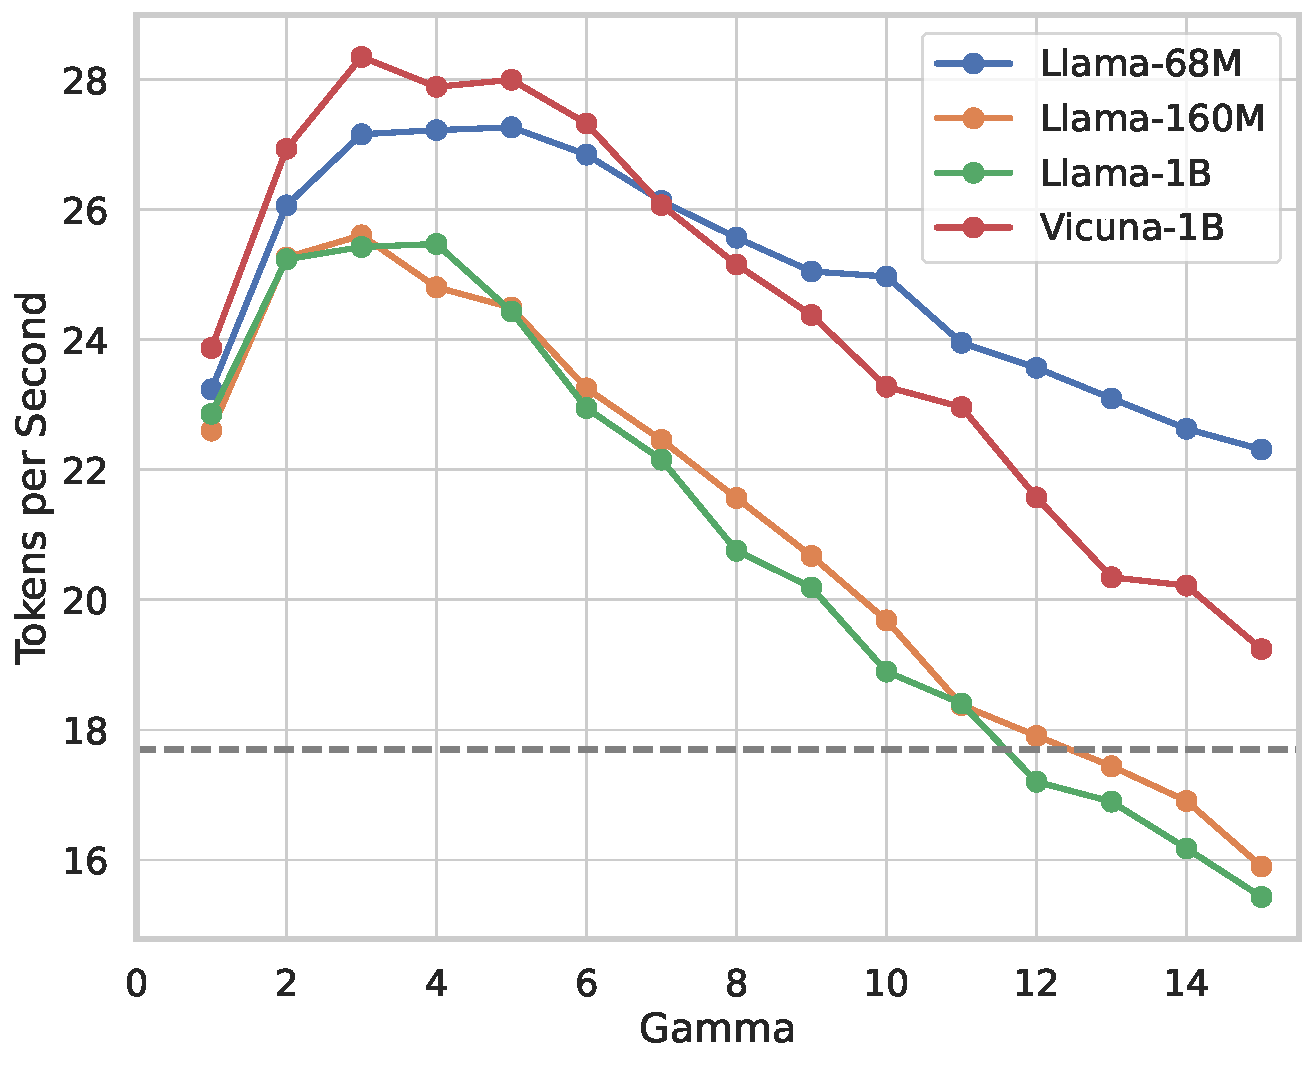
\includegraphics[width=\textwidth]{spec_33b.pdf}
         \caption{Vicuna-33B}
         \label{fig:spec33b}
     \end{subfigure}
        \caption{Inference speed of various models using speculative decoding on MT-Bench. Baseline model speeds are presented by grey dotted lines for comparison. $\gamma$ denotes the draft token number.}
        \label{fig:speculative_decoding}
\end{figure*}

\section{Additional Results for All Models}\label{appendix:add_results}
We show speedup on various models in Fig.~\ref{fig:speedup_model_wild}.
\begin{figure}[h]
    \centering
    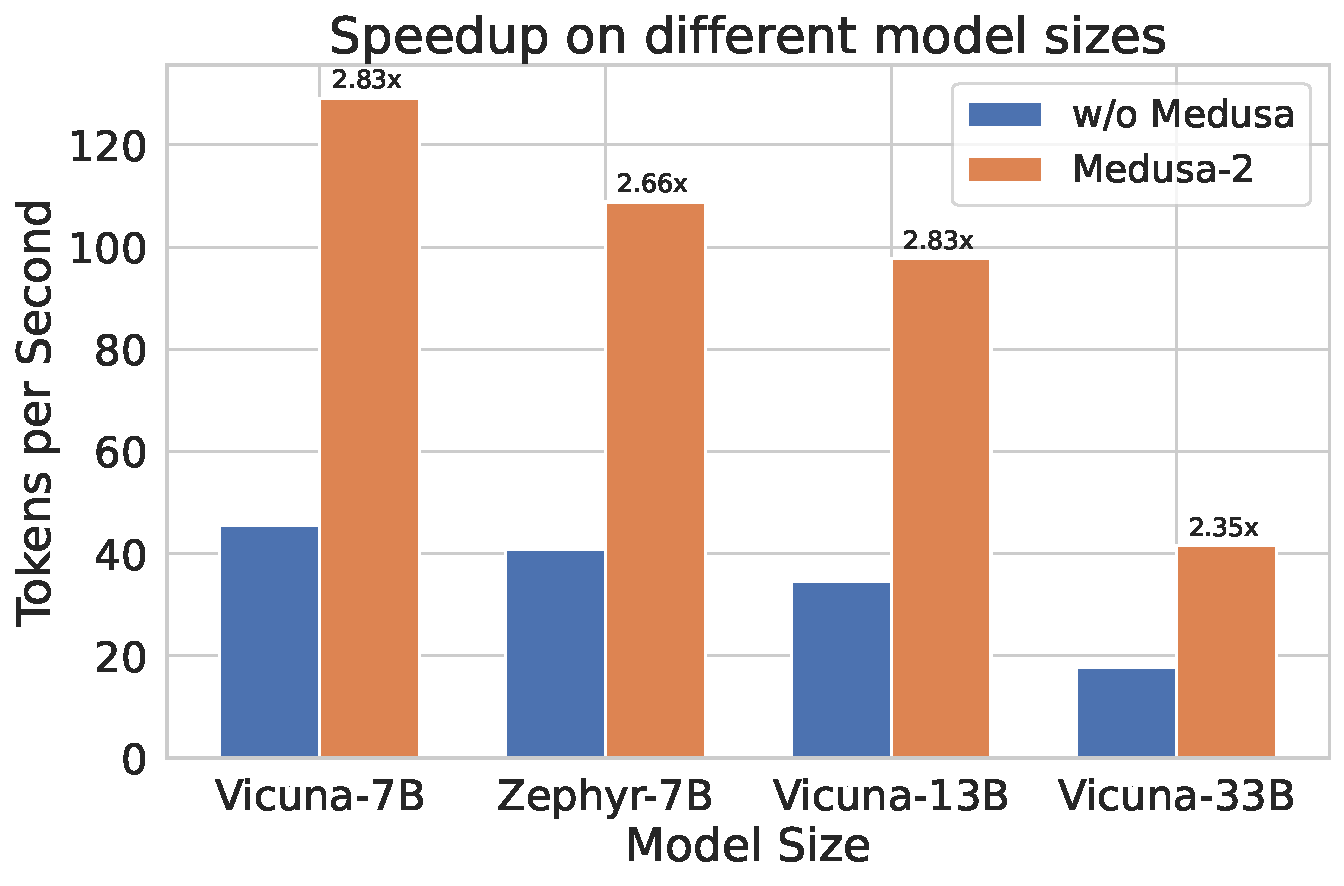
\includegraphics[width=0.45\textwidth]{speedup_model_wild_wide.pdf}
    \caption{Speedup of various models with \ours-2. \ours-2 shows significant speed improvement over all the models, while models trained with self-distillation \textcolor{black}{(Zephyr-7B, Vicuna-13/33B)} have weaker speedup due to the trade-off between preserving quality and boosting speed.}
    \label{fig:speedup_model_wild}
\end{figure}


\section{Additional Results on AlpacalEval Dataset}
We conduct further experiments on the AlpacaEval~\citep{alpaca_eval} dataset. \ours-2 achieves consistent speedup similar to the results on MT-Bench.
\begin{table}[h]
    \centering
    \begin{tabular}{llrrrr}
    \toprule
     & Model & Base speed (tokens/s) & \ours speed (tokens/s) & Acc. rate & Speedup \\
    \midrule
     & Vicuna-7b & 37.07 & 106.76 & 3.23 & 2.88 \\
     & Vicuna-13b & 29.01 & 91.54 & 3.28 & 3.16 \\
     & Vicuna-33b & 17.87 & 40.43 & 2.85 & 2.26 \\
     & Zephyr-7b & 34.21 & 99.50 & 3.08 & 2.91 \\
    \bottomrule
    \end{tabular}
    \caption{Speedup results on AlpacaEval~\citep{alpaca_eval} dataset.}
    \label{tab:alpaca_eval_speedup}
\end{table}

\section{Exploration and Modeling of Hardware Constraints and \ours}~\label{sec:roofline}


We explore the hardware constraints, specifically memory-bandwidth bound, and their impact on \ours-style parallel decoding by incorporating a simplified \textcolor{black}{Llama-series} model.
First, we \textcolor{black}{identify} that the operators involving matrix multiplications, such as linear layers and attention matrix multiplications, are the primary sources of overhead. We profile the performance of FLOP/s vs. Operational Intensity \textcolor{black}{which is the ratio of FLOP/s to bandwidth (bytes/s)}, across various GPUs, including the A100-80GB-PCIe, A40, and A6000.
Next, we examine the changes in FLOP/s vs. Operational Intensity when using \ours for different operators.
Finally, we apply a straightforward analytical model to calculate acceleration rates and combine it with hardware benchmarks. This provides insights into the effects under different model sizes, sequence lengths, and batch sizes.

\subsection{Roofline Model of Operators}
We present an analysis of the roofline model for various operators in large language models (LLMs), specifically focusing on Llama-7B, Llama-13B, and Llama-33B~\cite{touvron2023llama}. These models were benchmarked on different GPUs, including the A100-80GB-PCIe, A40, and A6000. We looked into the three categories of matrix multiplication operators since they represent the primary sources of computational overhead in these models. Our study follows the report~\cite{chen2023transformer} which investigates the effectiveness of batch size but ours focuses more on decoding and parallel decoding.

Table~\ref{tab:complexity} details the computation and space complexity for each operator during the prefill, decoding, and \ours decoding phases. The operators include the linear layers for query, key, and value matrices ($XW_{Q}$, $XW_{K}$, $XW_{V}$), the attention matrix multiplications ($QK^T$, $PV$), and the up/gate/down linear layers ($XW_{u}$, $XW_{g}$, $XW_{d}$).
$b$ stands for the batch size, $s$ stands for the sequence length, $h$ stands for the hidden dimension, $i$ stands for the intermediate dimension, $n$ stands for the number of attention heads, $d$ stands for the head dimension and $q$ stands for the candidate length for \ours.
For more details of these operators please refer to the articles~\cite{touvron2023llama, chen2023transformer}.


\begin{table}[h]
\centering
\caption{Computational and space complexity of the main operators in different phases. \textcolor{black}{The table is based on Table 2 in the report~\cite{chen2023transformer}.}}

\scriptsize
\begin{tabular}{lcccc}
\toprule
 \textbf{Operator} & \textbf{Input Shape} & \textbf{Output Shape} & \textbf{Comp. Complexity} & \textbf{Space Complexity} \\ \midrule
 \textbf{Prefill} \\ \midrule
 $XW_{Q}$, $XW_{K}$, $XW_{V}$ & $(b, s, h)$ & $(b, s, h)$ & $O(bsh^2)$ & $O(2bsh + h^2)$ \\ \midrule
  $QK^T$ & $(b, n, s, d),(b, n, s, d)$ & $(b, n, s, s)$ & $O(bs^2nd)$ & $O(2bsnd + bs^2n)$ \\ 
  $PV$ &$(b, n, s, s),(b, n, s, d)$&$(b, n, s, d)$&& \\ \midrule
  $XW_{u}$, $XW_{g}$ & $(b, s, h)$ & $(b, s, i)$ & $O(bshi)$ & $O(bs(h + i) + hi)$ \\ 
  $XW_{d}$&$(b, s, i)$&$(b, s, h)$&&\\ \midrule
   \textbf{Decoding} \\ \midrule
$XW_{Q}$, $XW_{K}$, $XW_{V}$ & $(b, 1, h)$ & $(b, 1, h)$ & $O(bh^2)$ & $O(2bh + h^2)$ \\ \midrule
  $QK^T$ & $(b, n, 1, d), (b, n, s, d)$ & $(b, n, s, 1)$ & $O(bsnd)$ & $O(bsn + bsnd + bnd)$ \\ 
  $PV$ & $(b, n, s, 1), (b, n, 1, d)$ & $(b, n, 1, d)$ & &  \\ \midrule
  $XW_{u}$, $XW_{g}$ & $(b, 1, h)$ & $(b, 1, i)$ & $O(bhi)$ & $O(b(h + i) + hi)$ \\
  $XW_{d}$ & $(b, 1, i)$ & $(b, 1, h)$ &  & \\\midrule
   \textbf{Parallel decoding} \\ \midrule
 $XW_{Q}$, $XW_{K}$, $XW_{V}$ & $(b, q, h)$ & $(b, q, h)$ & $O(bqh^2)$ & $O(2bqh + h^2)$ \\ \midrule
  $QK^T$ & $(b, n, q, d), (b, n, s, d)$ & $(b, n, s, q)$ & $O(bsqnd)$ & $O(bsqn + b(s+q)nd)$ \\ 
    $PV$ & $(b, n, s, q), (b, n, q, d)$ & $(b, n, q, d)$ & &  \\ \midrule
  $XW_{u}$, $XW_{g}$ & $(b, q, h)$ & $(b, q, i)$ & $O(bqhi)$ & $O(bq(h + i) + hi)$ \\
  $XW_{d}$ & $(b, q, i)$ & $(b, q, h)$ &  \\ \bottomrule
\end{tabular}
\label{tab:complexity}
\end{table}

Figures~\ref{fig:llama7b-roofline-a100}-\ref{fig:llama33b-roofline-a6000} show the benchmark of three categories of operators on different models (7/13/33B) under various settings. To evaluate each operator's performance and throughput, we chose the combination of settings including batch sizes from 1 to 64 in powers of 2 and sequence lengths from 128 to 8192 in powers of 2 \textcolor{black}{(49 settings for each operator)}. 
From all the figures, we observe that the datapoints of each operator in the prefill and decoding stages cluster at very similar positions across all GPUs and for various model sizes. 



During the prefill phase, increasing the batch size changes the FLOP/s of the attention matrix multiplications (see \texttt{`qk/pv init`}) but does not affect the Operational Intensity (refer to the vertical dashed arrow in Fig. 9). 
In contrast, increasing the sequence length impacts both FLOP/s and Operational Intensity in the prefill phase (refer to the diagonal dashed arrow in Fig. 9).
During the decoding phase, the attention matrix multiplications are significantly limited by memory bandwidth. Despite an increase in FLOP/s with changes in batch size and sequence length, the Operational Intensity remains nearly unchanged (see \texttt{`qk/pv ar`}). This indicates suboptimal resource utilization in the self-attention mechanism.

The linear layers in the prefill phase are mostly compute-bound (see \texttt{`qkv mlp init`} and \texttt{`up/gate/down init`}). During the decoding phase, the datapoints of the linear layer form a line with the same slope as the GPU’s memory bandwidth (see \texttt{`qkv mlp ar`} and \texttt{`up/gate/down ar`}). This indicates the linear layers in the decoding stage are also bounded by memory bandwidth. Increasing the batch size improves the achieved FLOP/s and Operational Intensity under memory bandwidth constraints through better parallelism. Note that linear layers only process the new token and are independent of sequence length (See `Decoding` section in Table~\ref{tab:complexity}).

\begin{figure}[h]
    \centering
    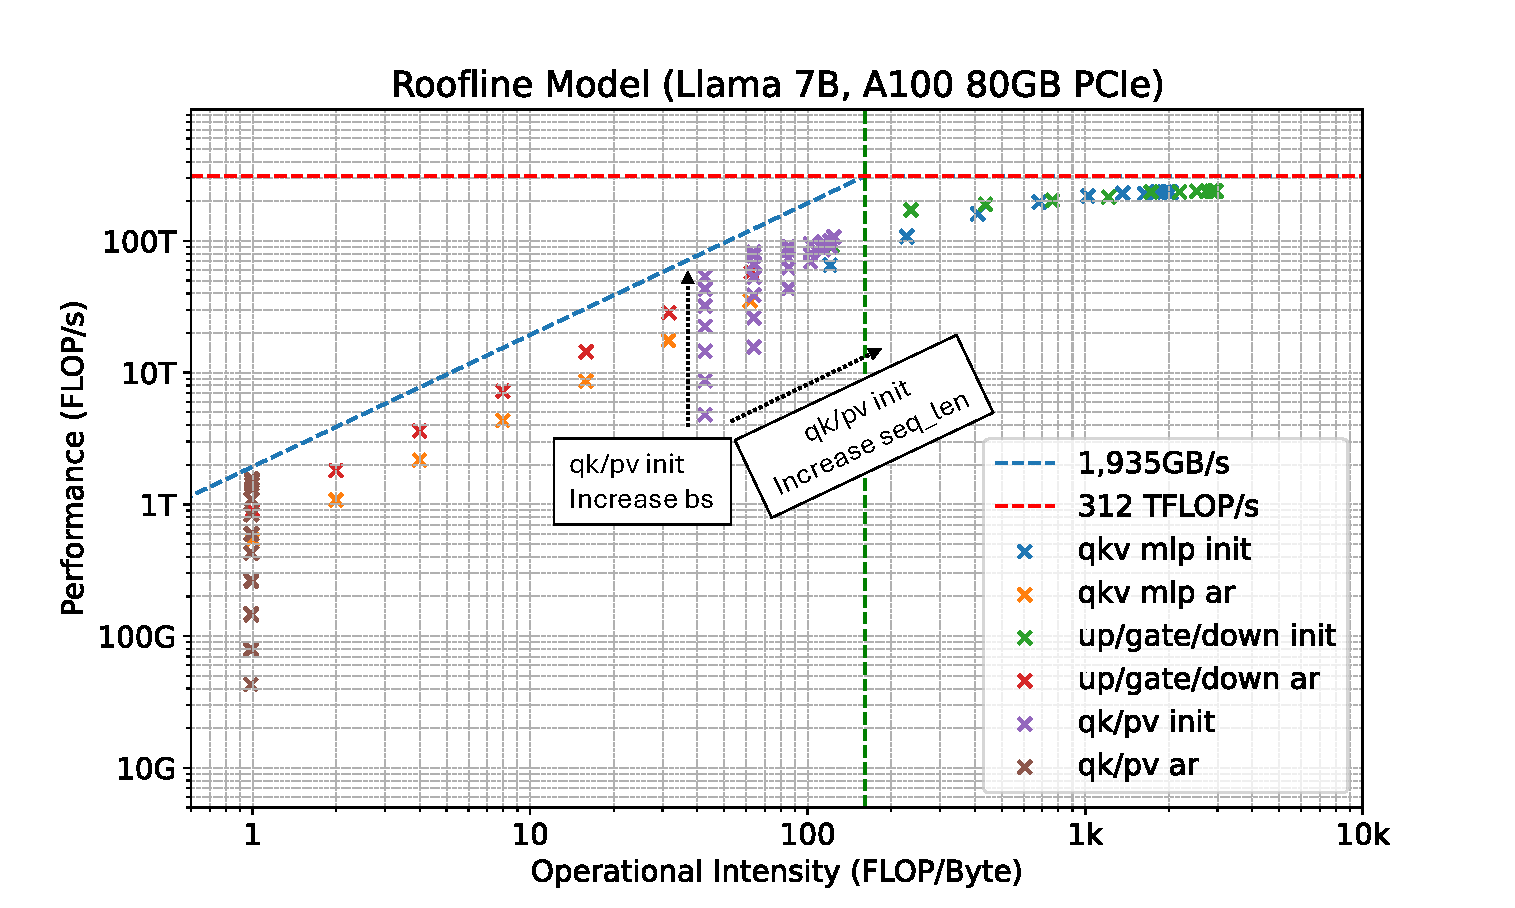
\includegraphics[width=0.8\textwidth]{llama7b-roofline-a100.pdf}
    \caption{The figure shows the relationship between FLOP/s and Operational Intensity for all benchmarked datapoints of Llama-7B operators on A100-80GB-PCIe. The dashed lines represent the HBM bandwidth limit (1,935GB/s) and the peak performance limit (312 TFLOP/s)~\cite{nvidia_a100_datasheet}. `\texttt{qkv mlp}' stands for the linear layers projecting hidden features to query/key/value features. `\texttt{up/gate/down}' stands for the linear layers following the attention block. `\texttt{qk/pv}' stands for the two steps of attention matrix multiplications. `\texttt{ar}' stands for the decoding (autoregressive) and `\texttt{init}' stands for the prefill phase.}
    \label{fig:llama7b-roofline-a100}
\end{figure}

\begin{figure}[h]
    \centering
    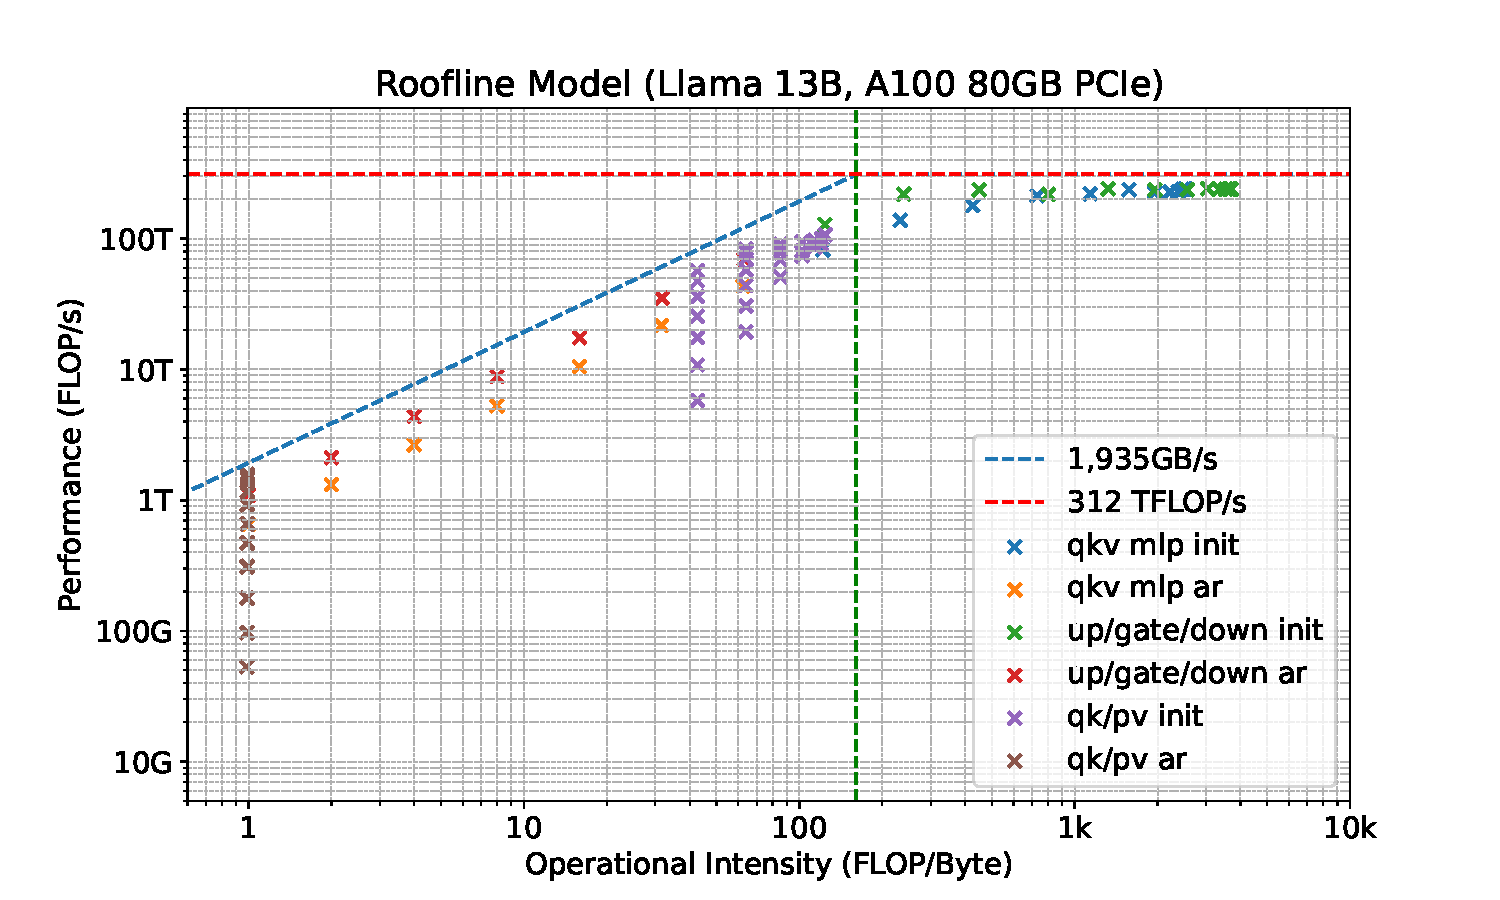
\includegraphics[width=0.8\textwidth]{llama13b-roofline-a100.pdf}
    \caption{Llama-13B operators on A100-80GB-PCIe.}
    \label{fig:llama13b-roofline-a100}
\end{figure}

\begin{figure}[h]
    \centering
    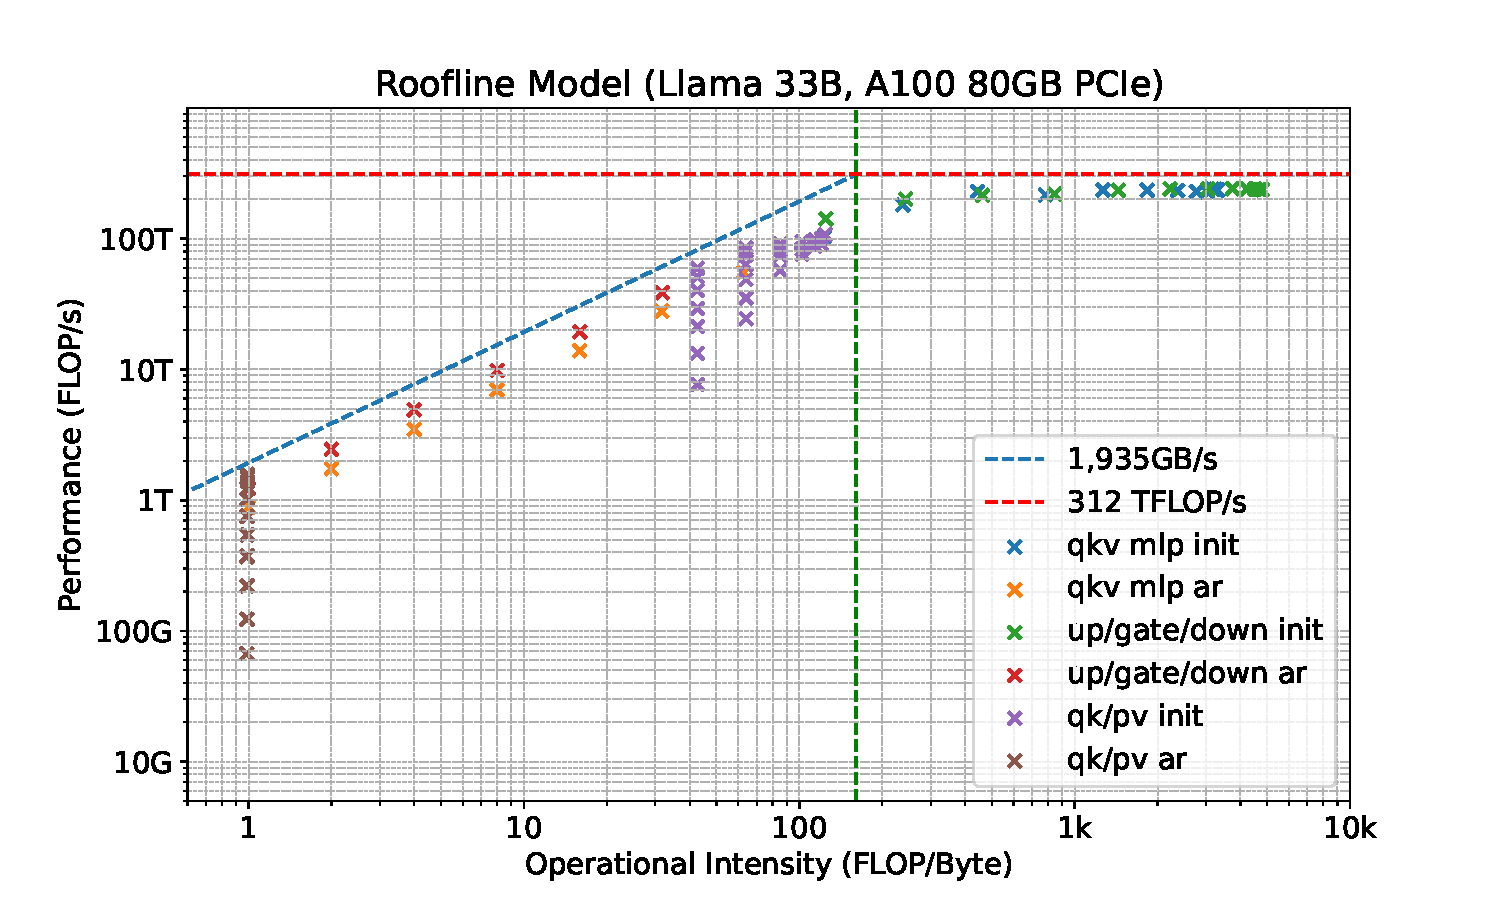
\includegraphics[width=0.8\textwidth]{llama33b-roofline-a100.pdf}
    \caption{Llama-33B operators on A100-80GB-PCIe.}
    \label{fig:llama33b-roofline-a100}
\end{figure}

\begin{figure}[h]
    \centering
    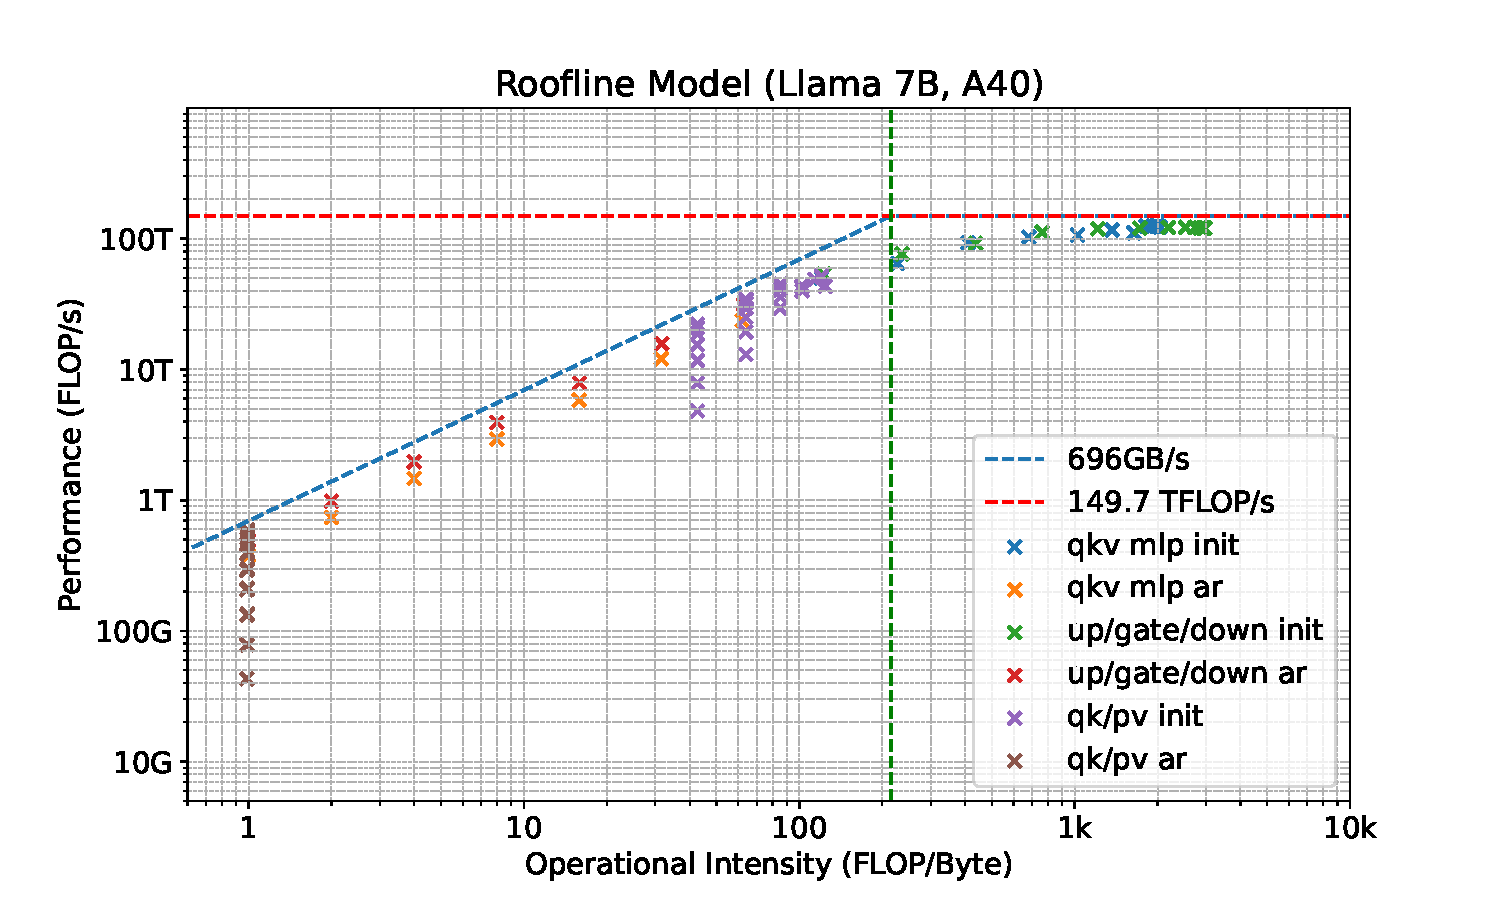
\includegraphics[width=0.8\textwidth]{llama7b-roofline-a40.pdf}
    \caption{Llama-7B operators on A40.}
    \label{fig:llama7b-roofline-a40}
\end{figure}


\begin{figure}[h]
    \centering
    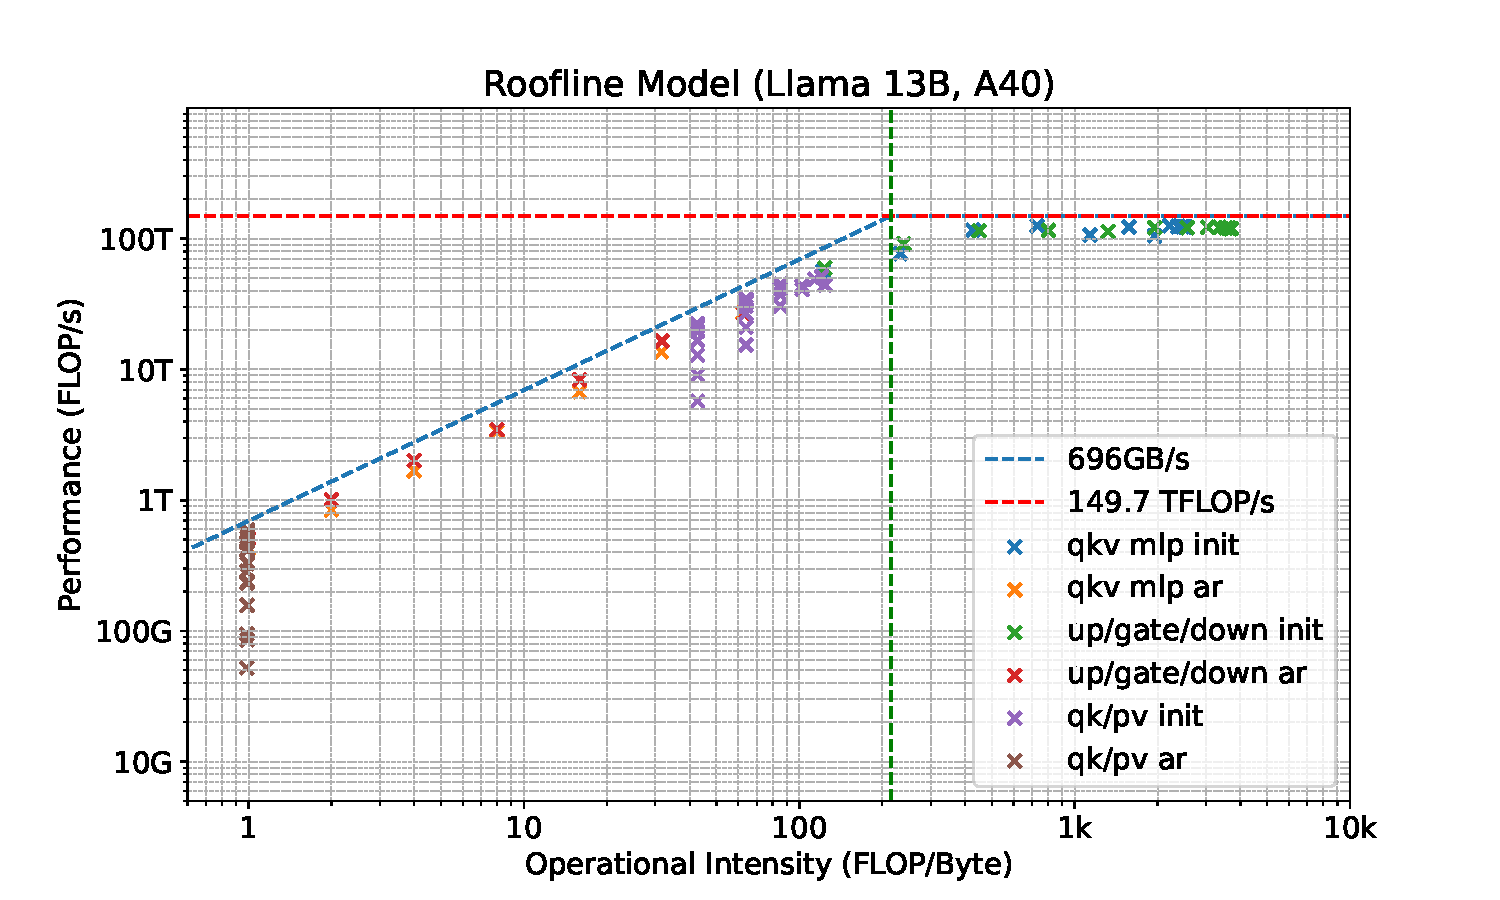
\includegraphics[width=0.8\textwidth]{llama13b-roofline-a40.pdf}
    \caption{Llama-13B operators on A40.}
    \label{fig:llama13b-roofline-a40}
\end{figure}


\begin{figure}[h]
    \centering
    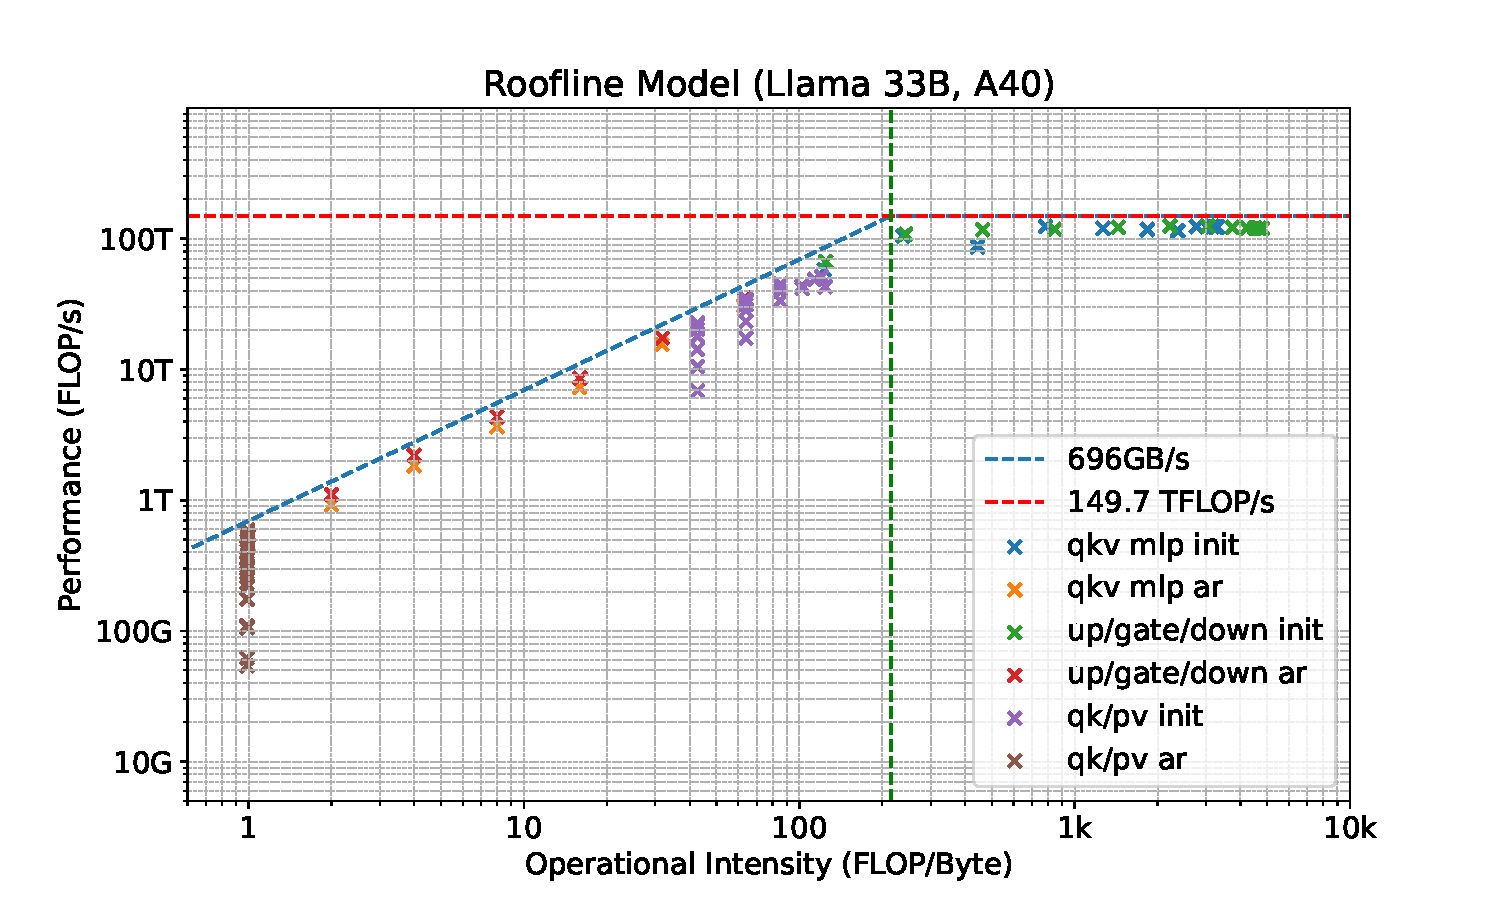
\includegraphics[width=0.8\textwidth]{llama33b-roofline-a40.pdf}
    \caption{Llama-33B operators on A40.}
    \label{fig:llama33b-roofline-a40}
\end{figure}



\begin{figure}[h]
    \centering
    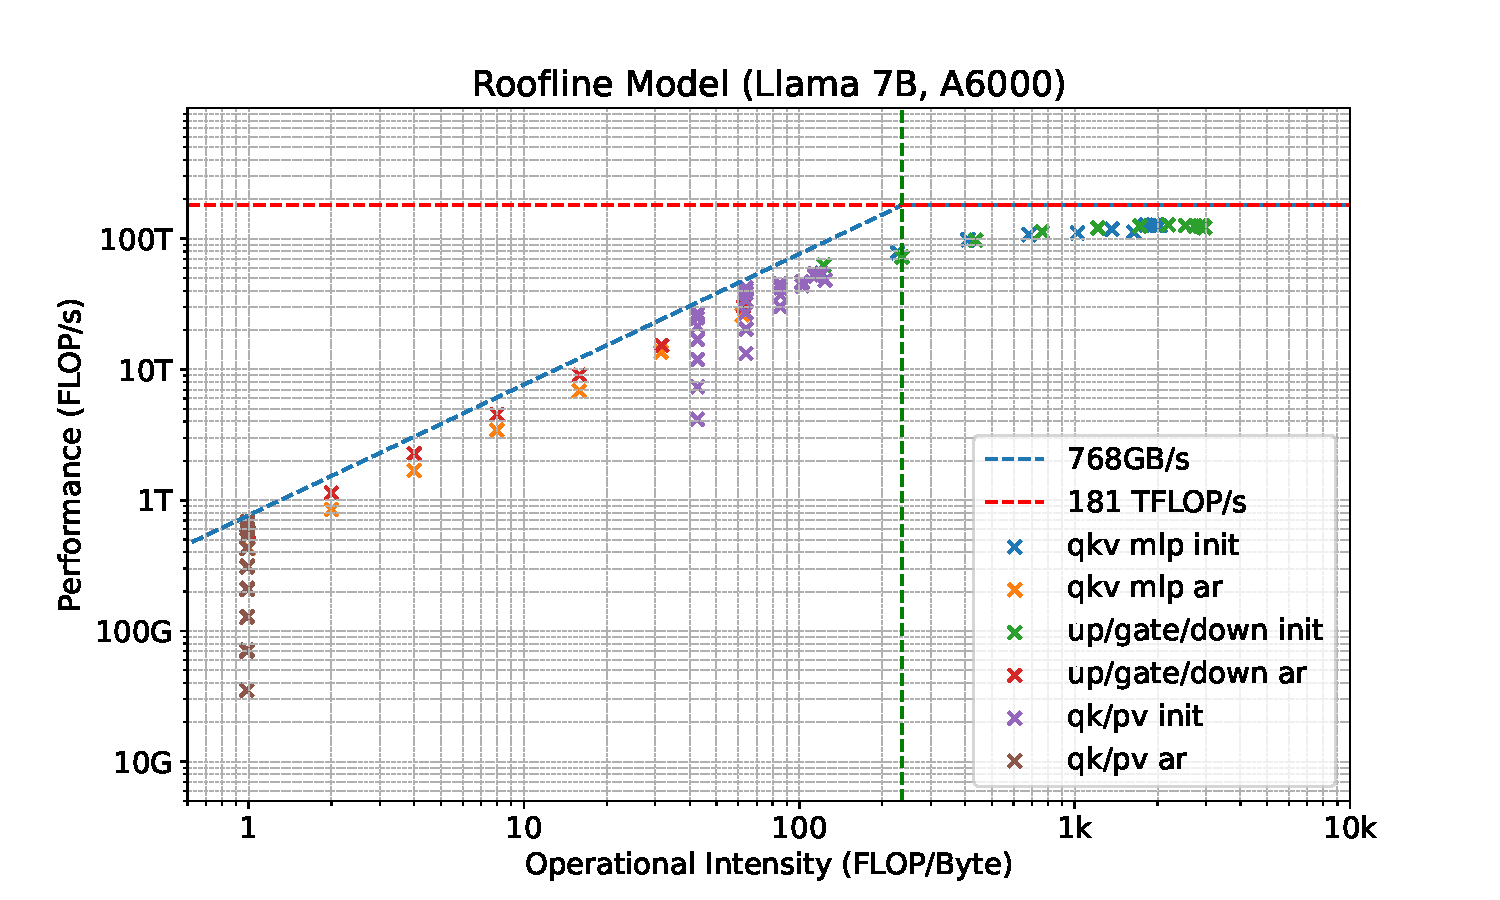
\includegraphics[width=0.8\textwidth]{llama7b-roofline-a6000.pdf}
    \caption{Llama-7B operators on A6000.}
    \label{fig:llama7b-roofline-a6000}
\end{figure}

\begin{figure}[h]
    \centering
    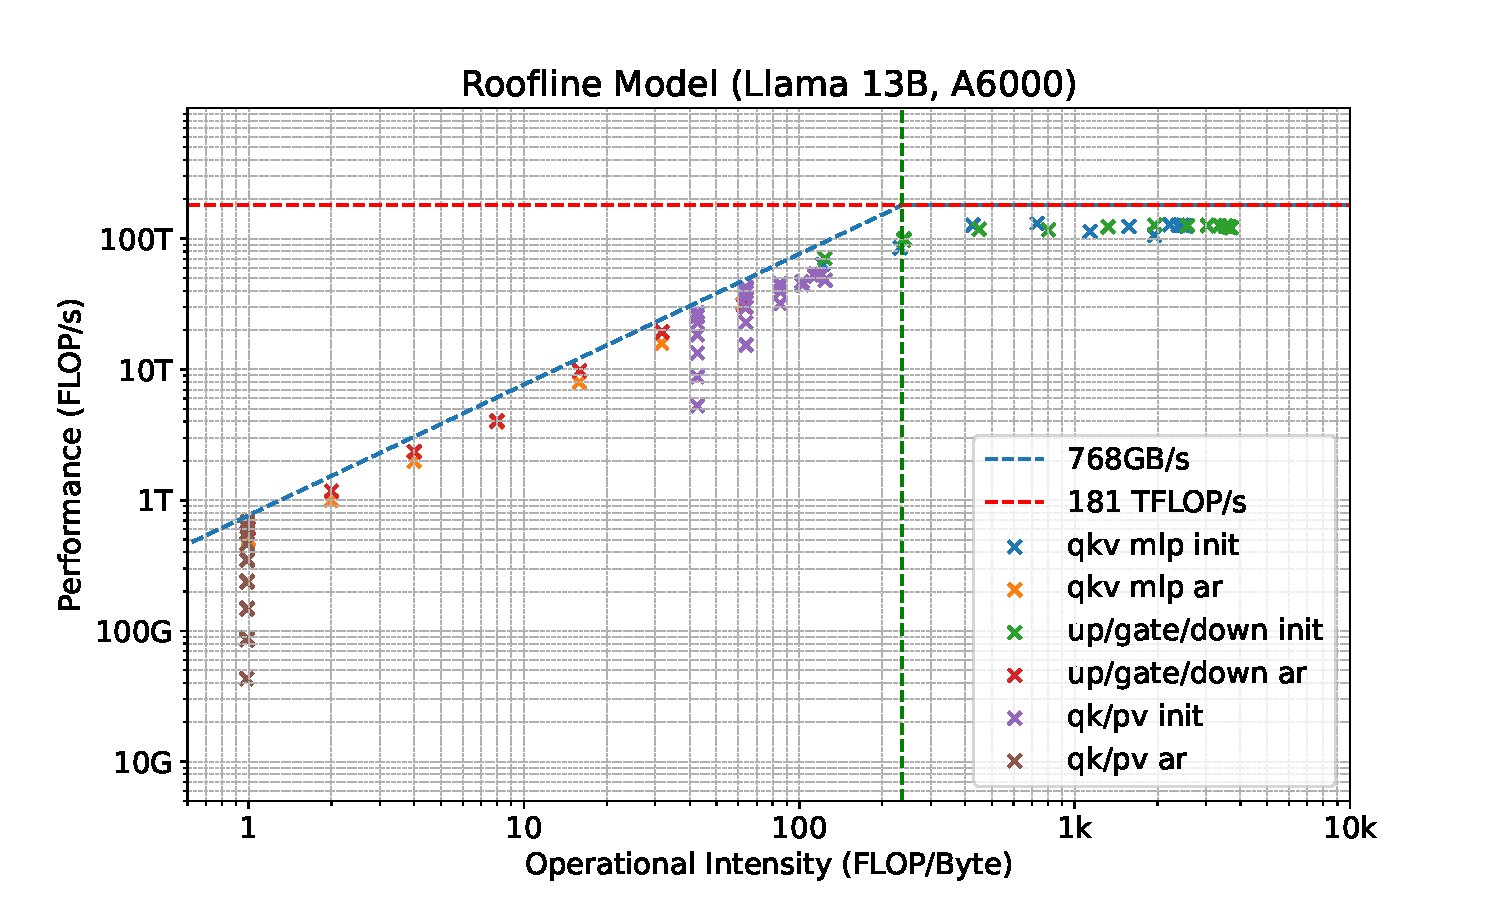
\includegraphics[width=0.8\textwidth]{llama13b-roofline-a6000.pdf}
    \caption{Llama-13B operators on A6000.}
    \label{fig:llama13b-roofline-a6000}
\end{figure}

\begin{figure}[h]
    \centering
    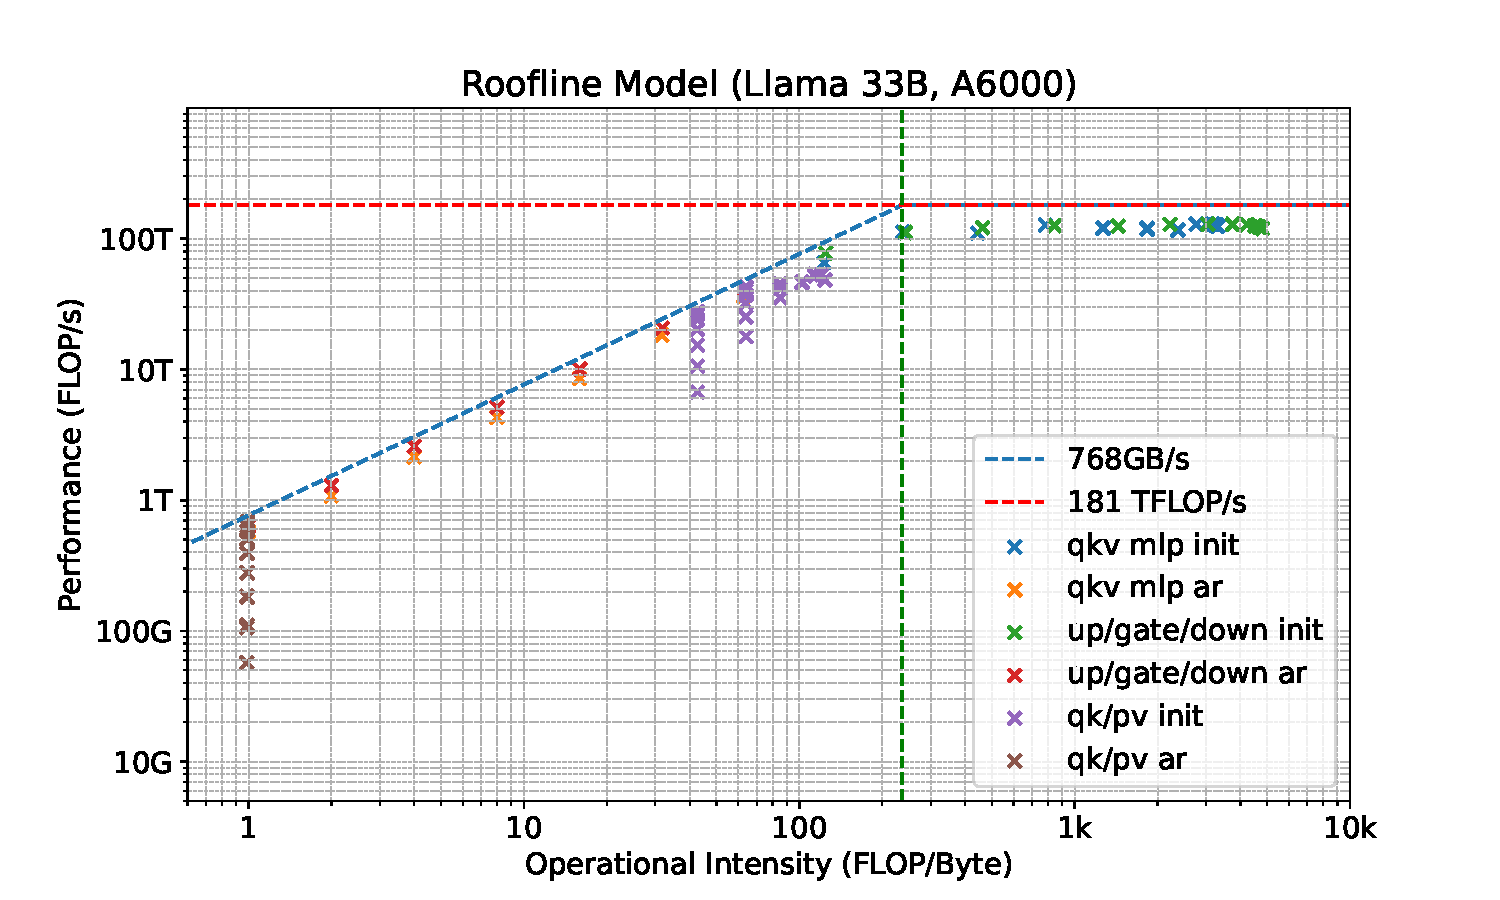
\includegraphics[width=0.8\textwidth]{llama33b-roofline-a6000.pdf}
    \caption{Llama-33B operators on A6000.}
    \label{fig:llama33b-roofline-a6000}
\end{figure}

\clearpage



\subsection{FLOP/s vs. Operational Intensity Variations in \ours}

We investigate how Medusa can change Operational Intensity and elevate the FLOP/s.
We choose Llama 33B on A100-80GB-PCIe as the setting. 

First, we examine the attention matrix multiplication. Fig.~\ref{fig:llama33b-spec-bs16} and Table~\ref{tab:llama33b-spec-bs16} illustrate the effects of \ours while keeping the batch size fixed at 16. We observe increased FLOP/s and Operational Intensity as more candidate tokens are added (original decoding results are plotted as grey dots). This indicates that \ours can leverage additional candidate tokens to improve computational throughput. Compared to regular decoding, \ours achieves 44$\times$ FLOP/s and 41$\times$ Operational Intensity under the setting of batch size 16 and sequence length 1024 with 64 candidate tokens.
 Fig.~\ref{fig:llama33b-spec-seq1024} and Table~\ref{tab:llama33b-spec-seq1024} illustrate the effects of \ours decoding while keeping the sequence length fixed at 1024. Increasing the batch size does not improve Operational Intensity in this scenario. 

Next, we examine the linear layer, focusing on the up/gate/down linear layers. The results are shown in Fig.~\ref{fig:llama33b-spec--mlp-bsall} and Table~\ref{tab:llama33b-spec--mlp-bsall}. \textcolor{black}{Since the linear layers in the decoding phase only process the future tokens while the past tokens are cached, they are independent of the sequence length.} We vary the batch size to observe the effects. As \ours increases the number of candidate tokens with the increasing batch size, we observe a shift from a memory-bandwidth-bound region to a computation-bound region. This shift demonstrates how \ours can transition the performance characteristics of the linear layers from being limited by memory bandwidth to being limited by computational capacity.

\begin{figure}[h]
    \centering
    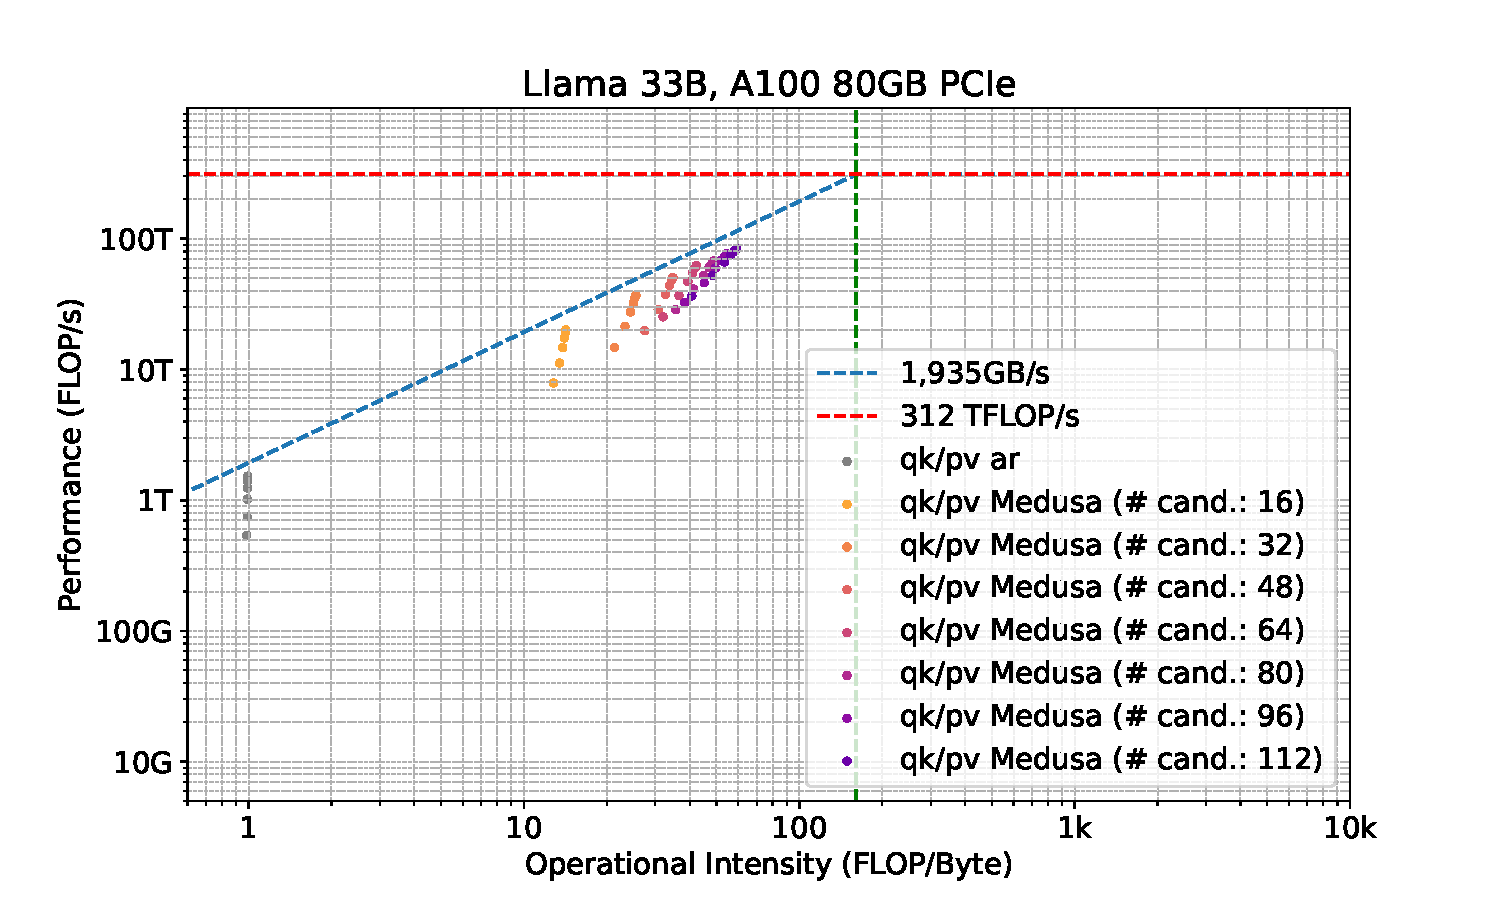
\includegraphics[width=0.8\textwidth]{llama33b-spec-bs16.pdf}
    \caption{FLOP/s vs. Operational Intensity of attention matrix multiplication with batch size 16.}
    \label{fig:llama33b-spec-bs16}
\end{figure}

\begin{figure}[h]
    \centering
    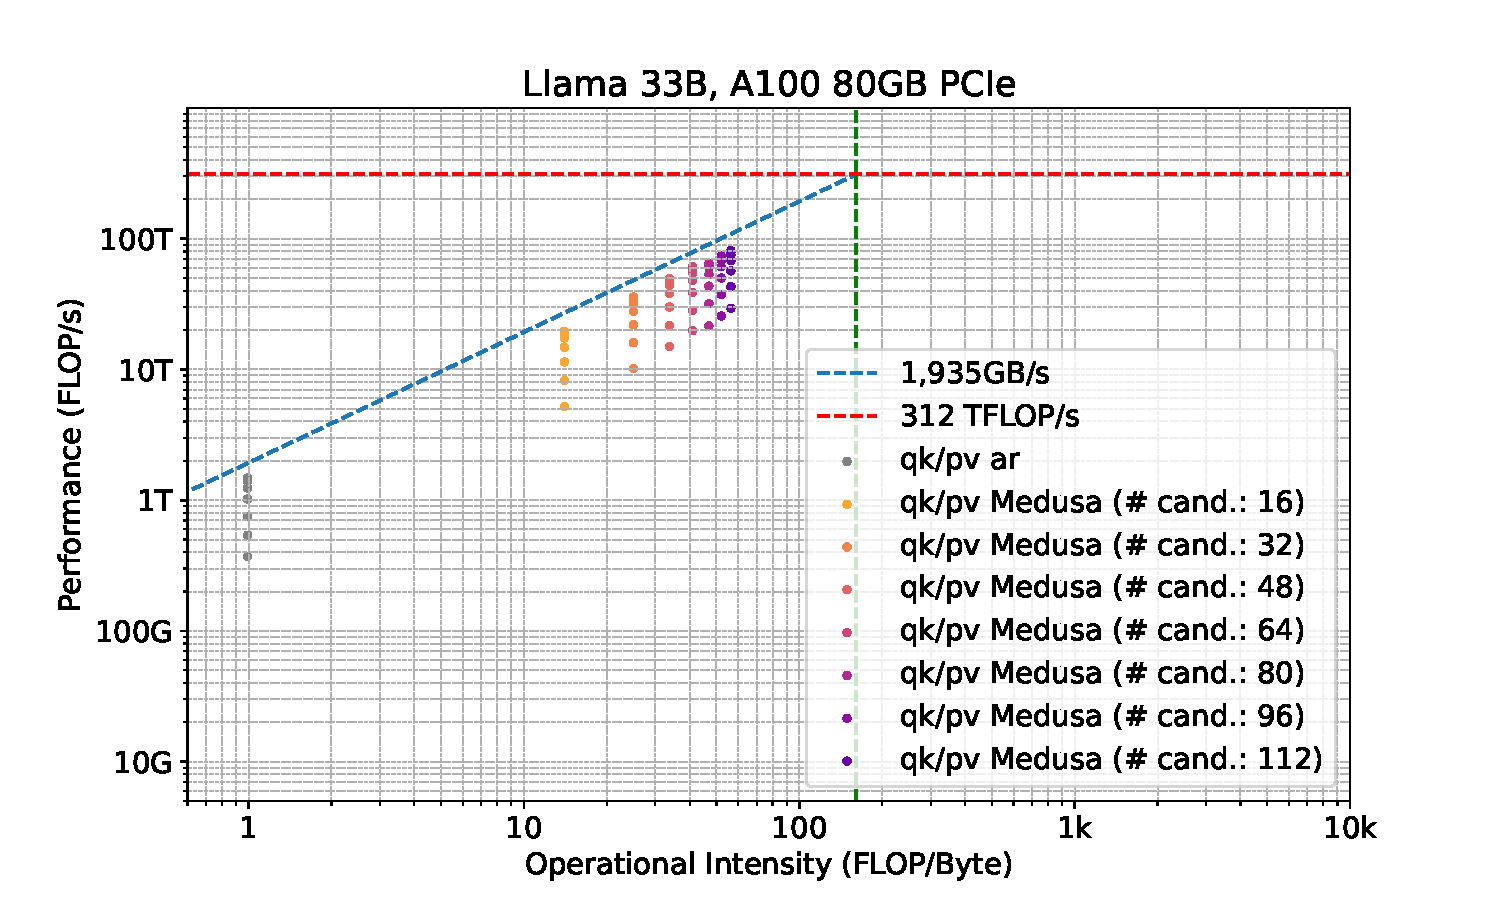
\includegraphics[width=0.8\textwidth]{llama33b-spec-seq1024.pdf}
    \caption{FLOP/s vs. Operational Intensity of attention matrix multiplication with sequence length 1024.}
    \label{fig:llama33b-spec-seq1024}
\end{figure}

\begin{figure}[h]
    \centering
    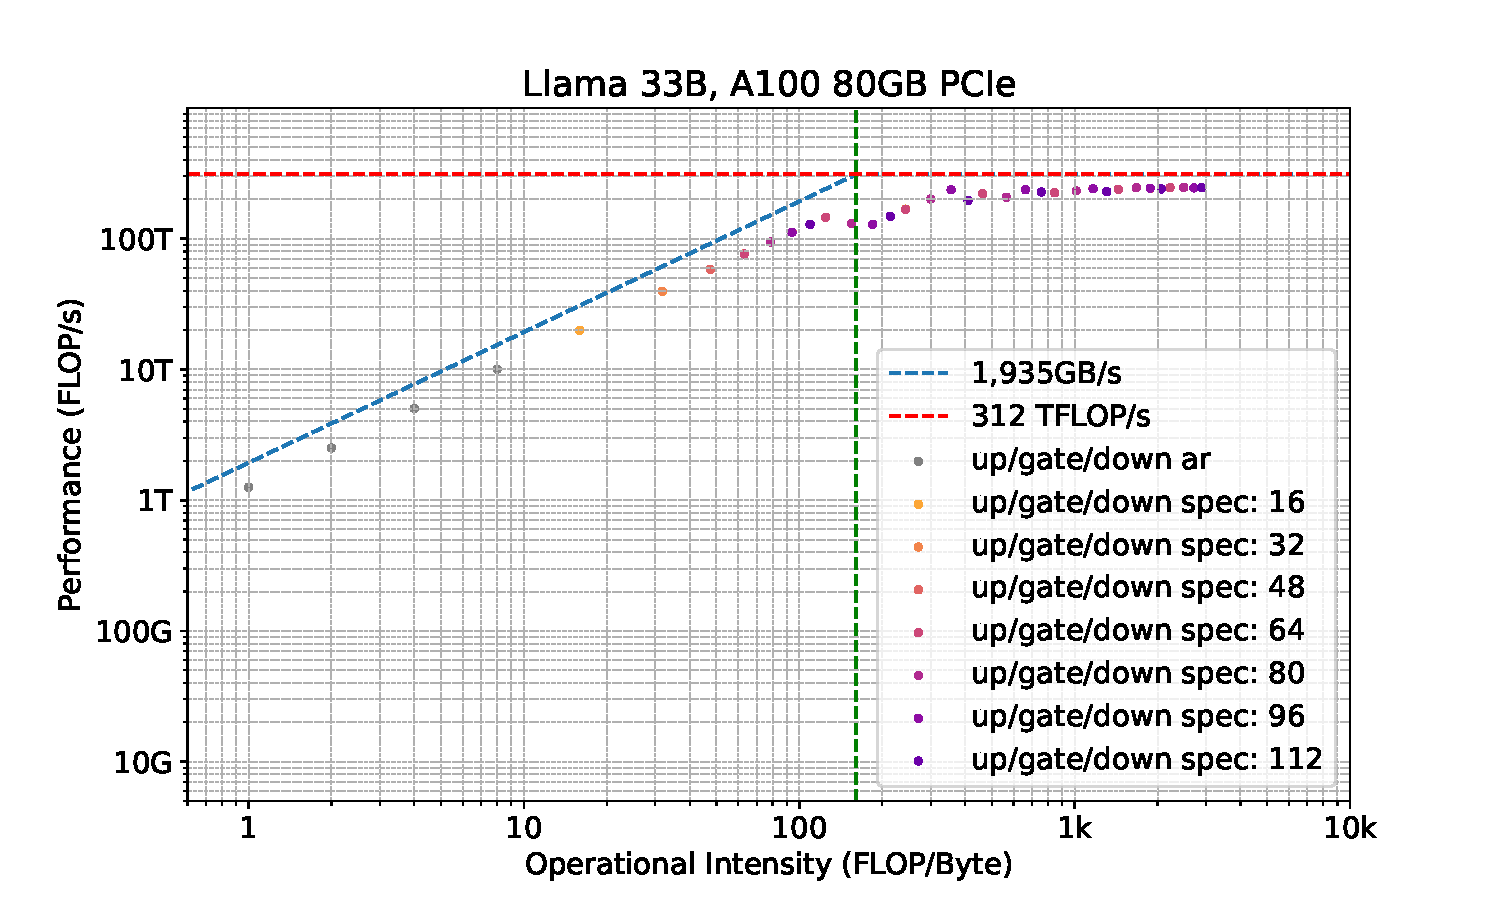
\includegraphics[width=0.8\textwidth]{llama33b-spec-mlp-bsall.pdf}
    \caption{FLOP/s vs. Operational Intensity of Linear layers.}
    \label{fig:llama33b-spec--mlp-bsall}
\end{figure}

\clearpage


\begin{table}[h]
\centering
\scriptsize
\begin{tabular}{lcccccccc}

\toprule
Seq. Length & \multicolumn{8}{c}{Number of Candidate Tokens} \\
\midrule
 & 1 & 16 & 32 & 48 & 64 & 80 & 96 & 112 \\
\midrule
128  & 0.54 \& 0.98 & 7.87 \& 12.8 & 14.73 \& 21.33 & 19.78 \& 27.43 & 25.25 \& 32.0 & 28.63 \& 35.56 & 32.58 \& 38.4 & 36.57 \& 40.73 \\
256  & 0.75 \& 0.99 & 11.2 \& 13.47 & 21.29 \& 23.27 & 28.69 \& 30.72 & 36.59 \& 36.57 & 41.2 \& 41.29 & 45.99 \& 45.18 & 52.33 \& 48.43 \\
512  & 1.02 \& 0.99 & 14.69 \& 13.84 & 27.47 \& 24.38 & 37.35 \& 32.68 & 47.09 \& 39.38 & 52.24 \& 44.91 & 59.55 \& 49.55 & 66.35 \& 53.49 \\
1024  & 1.24 \& 0.99 & 17.42 \& 14.03 & 32.15 \& 24.98 & 43.89 \& 33.76 & 54.8 \& 40.96 & 60.19 \& 46.97 & 68.28 \& 52.07 & 75.45 \& 56.44 \\
2048 & 1.39 \& 0.99 & 19.03 \& 14.12 & 35.05 \& 25.28 & 48.03 \& 34.32 & 59.66 \& 41.8 & 63.91 \& 48.08 & 72.83 \& 53.43 & 80.05 \& 58.04 \\
4096 & 1.48 \& 0.99 & 19.8 \& 14.17 & 36.59 \& 25.44 & 50.4 \& 34.61 & 62.29 \& 42.23 & 65.84 \& 48.65 & 74.86 \& 54.13 & 82.06 \& 58.87 \\
8192 & 1.53 \& 0.99 & 20.08 \& 14.2 & 36.89 \& 25.52 & 50.44 \& 34.76 & 62.11 \& 42.45 & 67.5 \& 48.94 & 76.97 \& 54.49 & 84.5 \& 59.3 \\
\bottomrule
\end{tabular}
\caption{
TFLOP/s \& Operational Intensity of attention matrix multiplication with batch size 16 for Llama 33B on an A100 80GB PCIe.}
\label{tab:llama33b-spec-bs16}
\end{table}


\begin{table}[h]
\centering
\scriptsize
\begin{tabular}{lcccccccc}
\toprule
Batch Size & \multicolumn{8}{c}{Number of Candidate Tokens} \\
\midrule
 & 1 & 16 & 32 & 48 & 64 & 80 & 96 & 112 \\
\midrule
1  & 0.37 \& 0.99 & 5.22 \& 14.03 & 10.15 \& 24.98 & 15.02 \& 33.76 & 19.79 \& 40.96 & 21.52 \& 46.97 & 25.65 \& 52.07 & 29.4 \& 56.44 \\
2  & 0.54 \& 0.99 & 8.25 \& 14.03 & 16.0 \& 24.98 & 21.62 \& 33.76 & 28.24 \& 40.96 & 31.84 \& 46.97 & 37.49 \& 52.07 & 43.04 \& 56.44 \\
4  & 0.75 \& 0.99 & 11.41 \& 14.03 & 21.97 \& 24.98 & 30.02 \& 33.76 & 38.71 \& 40.96 & 43.41 \& 46.97 & 50.06 \& 52.07 & 56.77 \& 56.44 \\
8  & 1.02 \& 0.99 & 14.78 \& 14.03 & 27.78 \& 24.98 & 38.09 \& 33.76 & 47.99 \& 40.96 & 53.32 \& 46.97 & 61.0 \& 52.07 & 68.11 \& 56.44 \\
16 & 1.24 \& 0.99 & 17.42 \& 14.03 & 32.15 \& 24.98 & 43.89 \& 33.76 & 54.8 \& 40.96 & 60.19 \& 46.97 & 68.28 \& 52.07 & 75.45 \& 56.44 \\
32 & 1.39 \& 0.99 & 18.89 \& 14.03 & 34.67 \& 24.98 & 47.57 \& 33.76 & 58.89 \& 40.96 & 63.61 \& 46.97 & 72.17 \& 52.07 & 79.21 \& 56.44 \\
64 & 1.48 \& 0.99 & 19.58 \& 14.03 & 35.87 \& 24.98 & 49.45 \& 33.76 & 61.13 \& 40.96 & 64.84 \& 46.97 & 73.73 \& 52.07 & 81.02 \& 56.44 \\

\bottomrule
\end{tabular}
\caption{
TFLOP/s \& Operational Intensity of attention matrix multiplication with sequence length 1024 for Llama 33B on an A100 80GB PCIe.}
\label{tab:llama33b-spec-seq1024}
\end{table}

\begin{table}[h]
\centering
\tiny
\begin{tabular}{lcccccccc}
\toprule
Batch Size & \multicolumn{8}{c}{Number of Candidate Tokens} \\
\midrule
 & 1 & 16 & 32 & 48 & 64 & 80 & 96 & 112 \\
\midrule
1  & 1.26 \& 1.0 & 19.95 \& 15.95 & 39.69 \& 31.79 & 58.4 \& 47.53 & 76.57 \& 63.17 & 94.4 \& 78.7 & 111.91 \& 94.14 & 128.64 \& 109.47 \\
2  & 2.51 \& 2.0 & 39.66 \& 31.79 & 76.53 \& 63.17 & 112.05 \& 94.14 & 145.73 \& 124.71 & 130.67 \& 154.89 & 129.1 \& 184.69 & 148.56 \& 214.12 \\
4  & 5.03 \& 4.0 & 76.44 \& 63.17 & 145.8 \& 124.71 & 128.85 \& 184.69 & 167.85 \& 243.17 & 201.19 \& 300.21 & 236.93 \& 355.85 & 195.91 \& 410.14 \\
8  & 10.06 \& 7.99 & 145.72 \& 124.71 & 168.26 \& 243.17 & 236.83 \& 355.85 & 221.11 \& 463.14 & 207.79 \& 565.44 & 236.95 \& 663.07 & 227.8 \& 756.36 \\
16 & 19.96 \& 15.95 & 168.35 \& 243.17 & 221.41 \& 463.14 & 237.5 \& 663.07 & 224.71 \& 845.59 & 232.49 \& 1012.87 & 241.12 \& 1166.74 & 229.25 \& 1308.76 \\
32 & 39.69 \& 31.79 & 221.74 \& 463.14 & 224.88 \& 845.59 & 241.33 \& 1166.74 & 239.02 \& 1440.25 & 245.83 \& 1675.97 & 243.55 \& 1881.24 & 240.33 \& 2061.59 \\
64 & 76.57 \& 63.17 & 225.19 \& 845.59 & 239.2 \& 1440.25 & 243.26 \& 1881.24 & 246.16 \& 2221.31 & 246.91 \& 2491.55 & 244.52 \& 2711.46 & 246.14 \& 2893.91 \\
\bottomrule
\end{tabular}
\caption{
TFLOP/s \& Operational Intensity of linear layers (up/gate/down) for Llama 33B on an A100 80GB PCIe.
}\label{tab:llama33b-spec--mlp-bsall}
\end{table}

\subsection{Predicting \ours Performance}

We further employ a straightforward analytical model \textcolor{black}{for} the acceleration rate. The ablation study results in Sec.~\ref{section:config of tree} indicate that the acceleration rate can be approximated by a simple logarithmic function. Using the results from Fig.~\ref{fig:sparse_acc}, we model the curve as $\texttt{acc\_rate} = 0.477 \log(\texttt{num\_candidate})$. We simulate the latency of one simplified block of the Llama-7B model (sequentially processing $XW_Q$, $XW_K$, $XW_V$, $QK^T$, $PV$, $XW_u$, $XW_g$, $XW_d$) by first fixing the batch size at 1 and the sequence length at 1024.
\textcolor{black}{
The candidate tokens are processed parallelly by constructing the tree attention described in Section~\ref{sec:tree_attention}. We omit the latency of the post-processing steps including verification and acceptance for \ours since they introduce marginal overhead.
}
Fig.~\ref{fig:llama7b-sim-bs1-seq1024} illustrates the simulated acceleration rate and speedup for different numbers of candidate tokens under these settings. As the number of candidate tokens increases, both the acceleration rate and speedup initially show improvements. However, beyond 64, the speedup starts to decline, indicating diminishing returns with further increases in candidate length. This aligns with the experimental results in Fig.~\ref{fig:sparse_speed} and suggests that there is an optimal range for the numbers of candidate tokens where \ours provides the most significant performance gains.

We plot the simulated speedup under different batch size settings with a fixed sequence length of 1024 in Fig.~\ref{fig:llama7b-sim-bs1-allbs}. The results indicate that when the batch size exceeds 32, the speedup decreases and may even have a negative effect. This occurs because the linear layers shift from being memory-bandwidth-bound to computationally bound.

We conduct another experiment using a batch size of 4 and different sequence lengths. As shown in Fig.~\ref{fig:llama7b-sim-allseq}, the optimal number of candidate tokens remains relatively consistent across different sequence lengths. However, as the sequence length increases, the overall performance decreases. This performance drop is primarily due to the overhead from attention matrix multiplication, while the linear layer computation remains constant \textcolor{black}{since the computation of linear layers is independent of the sequence length.}

Our simulations show that the optimal number of candidate tokens is key for model scaling with \ours, as benefits decrease beyond a certain range. Initially, increasing batch size improves performance through parallelism, but too large a batch size shifts linear layers from memory-bandwidth-bound to compute-bound, reducing speedup. Longer sequences increase attention matrix multiplication overhead, lowering performance, and emphasizing the need to optimize attention mechanisms. Effective model scaling requires balancing the number of candidate tokens, adjusting batch sizes to avoid compute-bound transitions, and enhancing attention mechanisms for longer sequences. These strategies ensure better resource utilization and higher performance, demonstrating the value of simulations in predicting performance and guiding acceleration strategy design.

\begin{figure}[h]
    \centering
    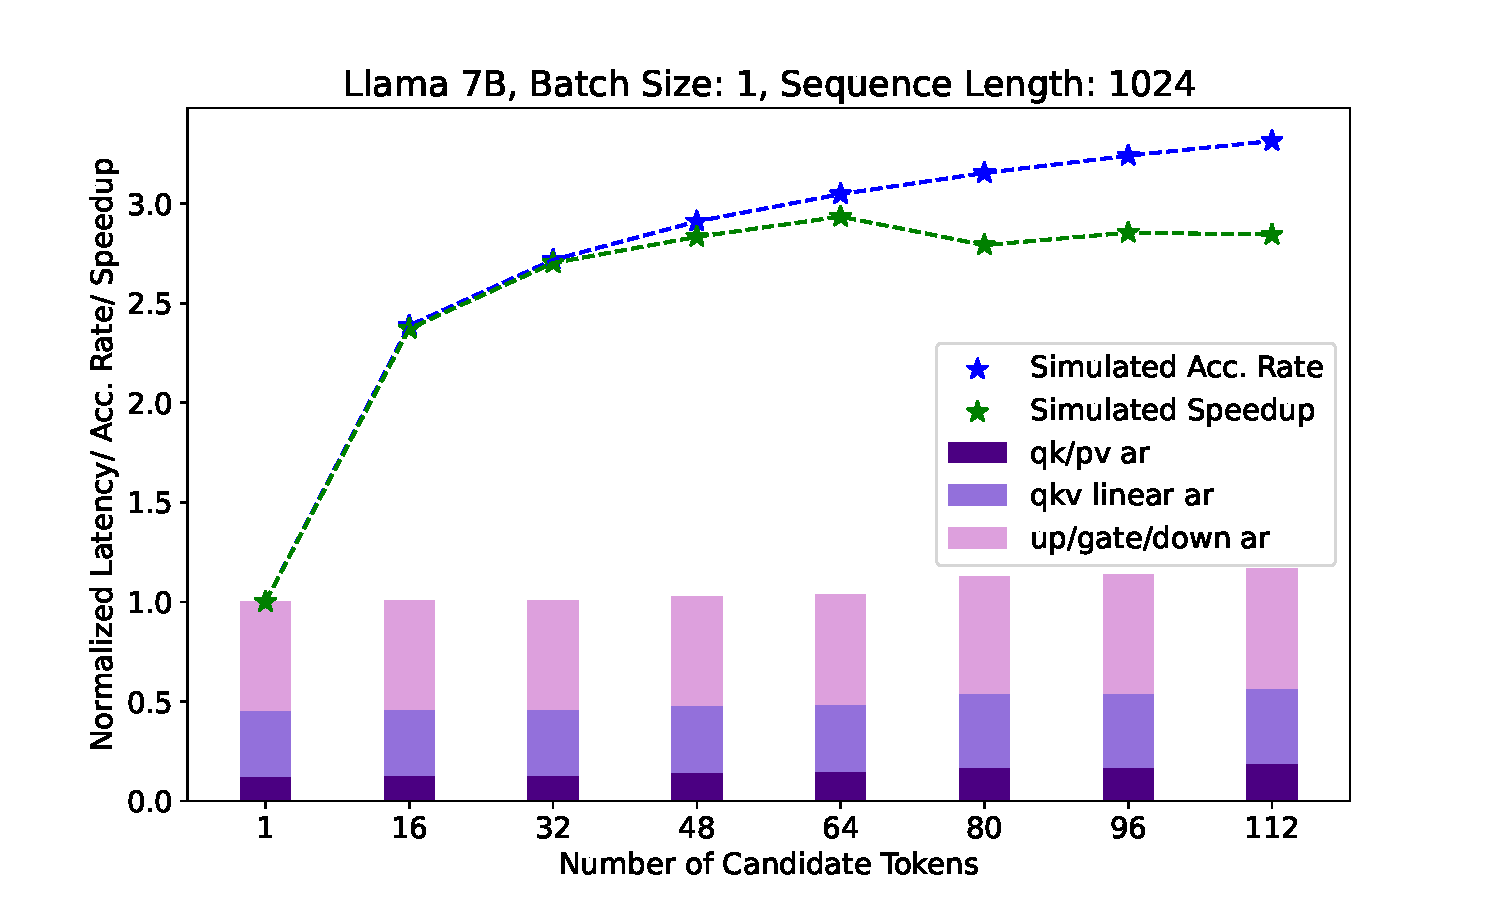
\includegraphics[width=0.8\textwidth]{llama7b-sim-bs1-seq1024.pdf}
    \caption{Simulated acceleration rate, speedup, and normalized latency ablation using different numbers of candidate tokens under the setting of batch size 1 and sequence length 1024 for Llama-7B on an A100 80GB PCIe.}
    \label{fig:llama7b-sim-bs1-seq1024}
\end{figure}

\begin{figure}[h]
    \centering
    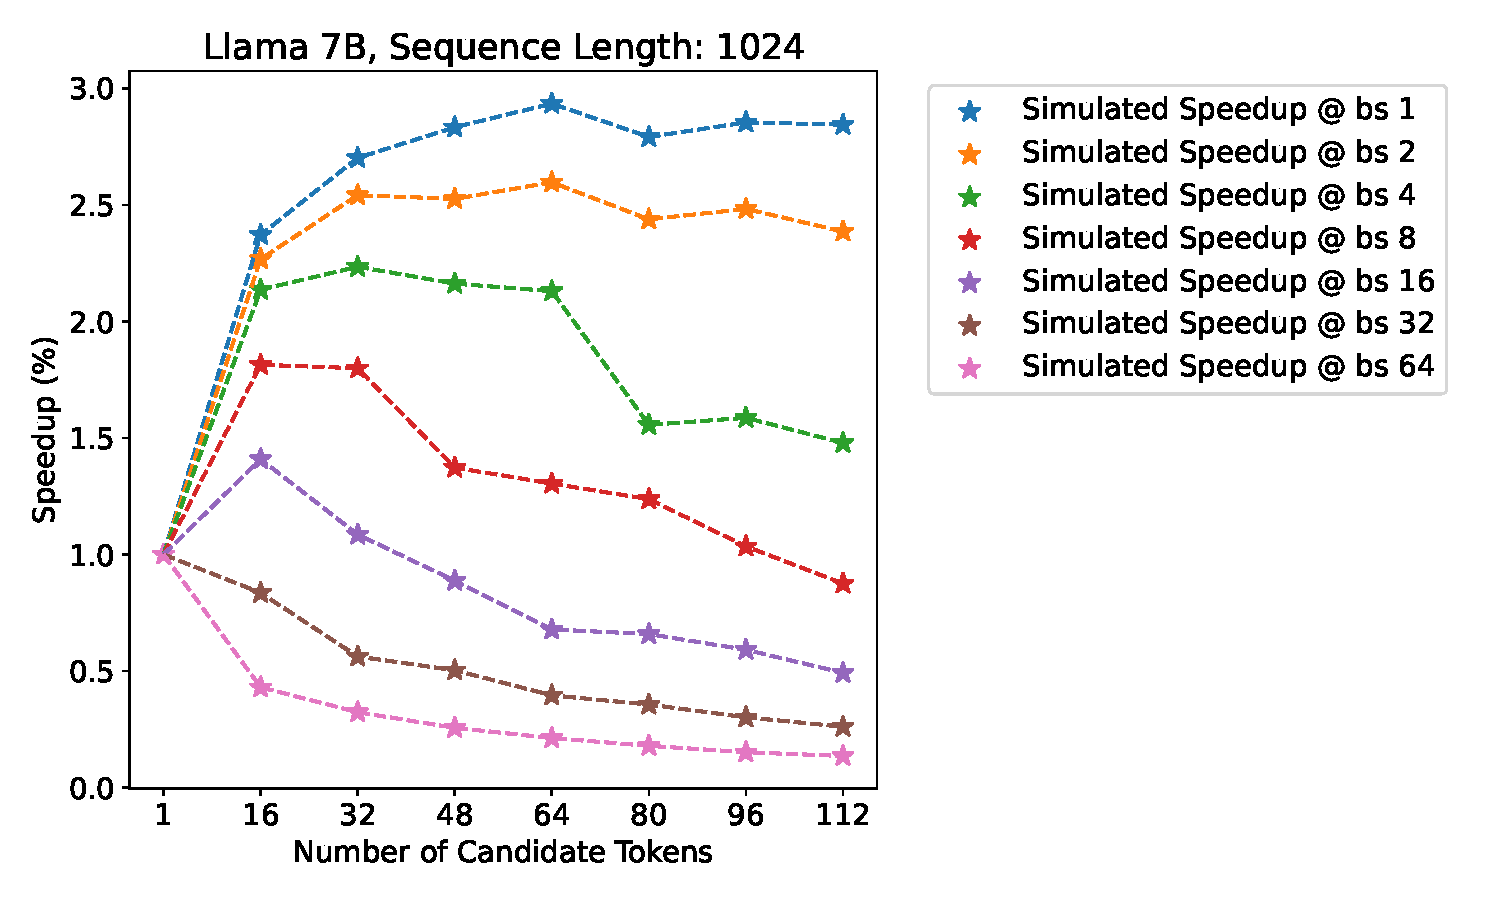
\includegraphics[width=0.8\textwidth]{llama7b-sim-allbs.pdf}
    \caption{Simulated speedup with sequence length 1024 for Llama-7B.}
    \label{fig:llama7b-sim-bs1-allbs}
\end{figure}

\begin{figure}[h]
    \centering
    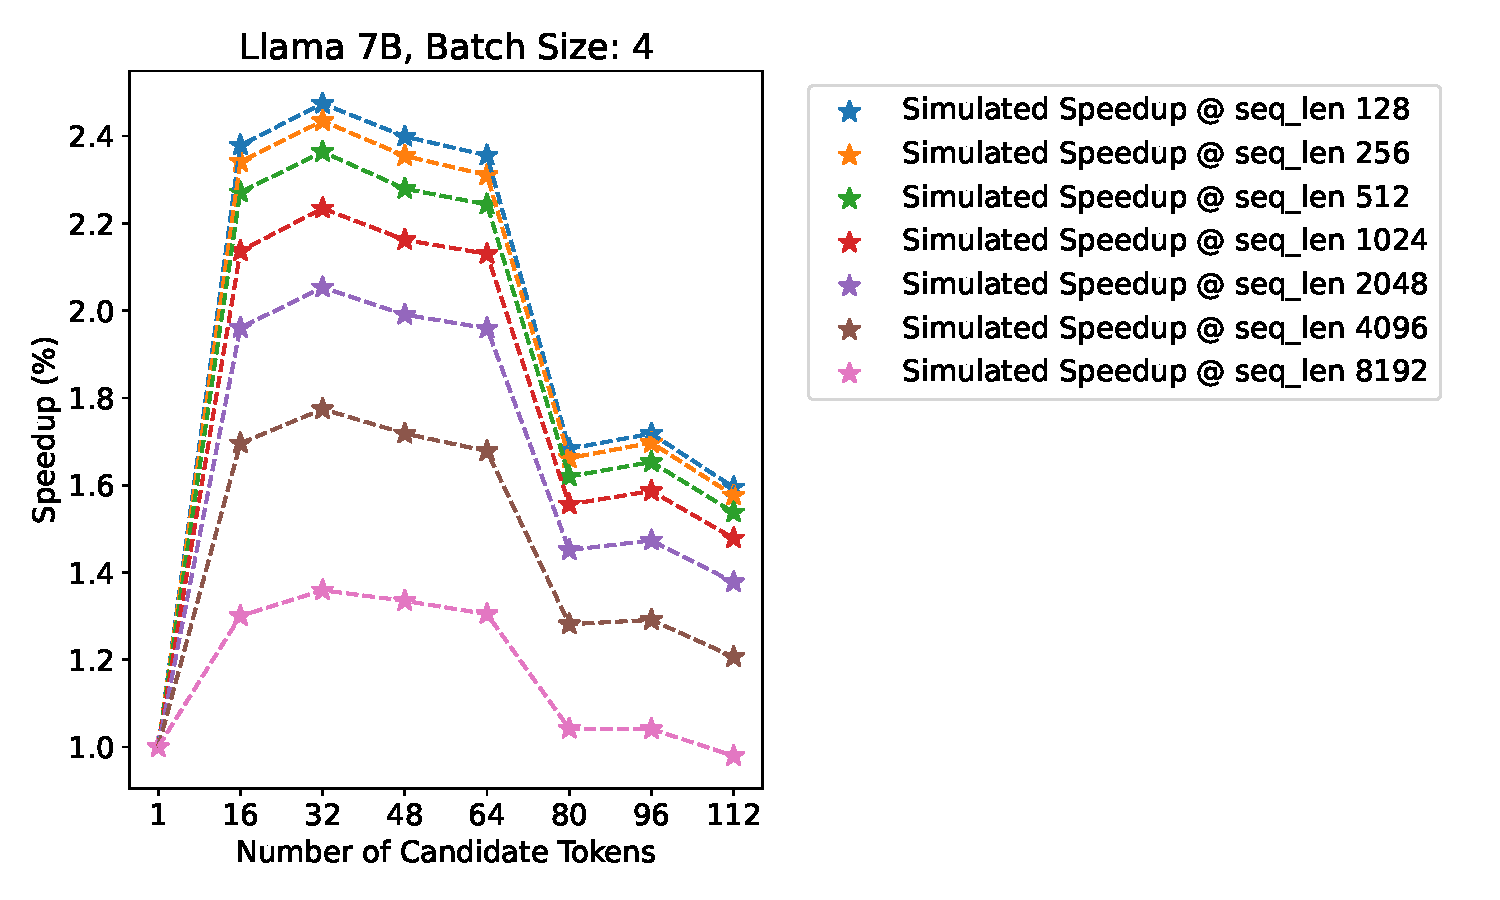
\includegraphics[width=0.8\textwidth]{llama7b-sim-allseq.pdf}
    \caption{Simulated speedup with batch size 4 for Llama-7B.}
    \label{fig:llama7b-sim-allseq}
\end{figure}
\end{document}